%% LaTeX2e class for student theses
%% thesis.tex
%% 
%% Karlsruhe Institute of Technology
%% Institute for Program Structures and Data Organization
%% Chair for Software Design and Quality (SDQ)
%%
%% Dr.-Ing. Erik Burger
%% burger@kit.edu
%%
%% See https://sdq.kastel.kit.edu/wiki/Dokumentvorlagen
%%
%% Version 1.6, 2024-06-07

%% Available page modes: oneside, twoside
%% Available languages: english, ngerman
%% Available modes: draft, final (see README)
\documentclass[twoside, english, final]{sdqthesis}
\usepackage{pgfgantt}
\usepackage{verbatim}
\usepackage{fancyvrb}
\usepackage{float}
\usepackage[final]{listings}
\usepackage{xcolor}

%% Colors of the listings
\definecolor{lstkeyword}{HTML}{003D99}
\definecolor{lstannotation}{HTML}{00706B}
\definecolor{lststring}{HTML}{A31515}
\definecolor{lstcomment}{HTML}{6E6E6E}
\definecolor{lstnumber}{HTML}{808080}
\definecolor{lstframe}{HTML}{B0B0B0}

%% The Reactions Language. The keywords are the terminals of ReactionsLanguage.xtext,
%% the third class holds the Xbase keywords that occur inside routine bodies.
\lstdefinelanguage{reactions}{
  morekeywords={absence, actions, after, and, anychange, as, asserted, at, attribute,
      call, changes, check, corresponding, create, created, deleted, element, execute,
      from, import, in, inserted, many, match, names, new, of, optional, plain, qualified,
      reaction, reactions, removed, replaced, require, retrieve, root, routine, routines,
      tagged, to, update, using, val, with},
  morekeywords=[2]{@feature, type},
  morekeywords=[3]{if, else, var, return, for, while, do, switch, case, default, try,
      catch, finally, throw, typeof, instanceof, extends, super, this, static, extension,
      synchronized, true, false, null},
  alsoletter={@},
  sensitive=true,
  morecomment=[l]{//},
  morecomment=[s]{/*}{*/},
  morestring=[b]{"},
}

%% Xtend, as far as the test gate listing needs it
\lstdefinelanguage{xtend}[]{Java}{
  morekeywords={def, val, var, extension, override, dispatch},
  morekeywords=[2]{@Test, @RequiresFeatures, @IncompatibleFeatures},
  alsoletter={@},
}

%% Only the colors. Layout stays with the options given at each listing.
\lstset{
  basicstyle=\ttfamily,
  keywordstyle=\color{lstkeyword}\bfseries,
  keywordstyle=[2]\color{lstannotation}\bfseries,
  keywordstyle=[3]\color{lstkeyword},
  stringstyle=\color{lststring},
  commentstyle=\color{lstcomment}\itshape,
  showstringspaces=false,
}
\usepackage{makecell}
\usepackage{tabularx}
\usepackage[figuresright]{rotating}
\usepackage{amsfonts}
\usepackage{todonotes}
%% Keep "--" in typewriter text, e.g. command-line flags, as two hyphens instead of an en dash
\DisableLigatures[-]{encoding = T1, family = tt*}
%% \autoref for the beginning of a sentence, capitalizing the names hyperref writes in lowercase
\newcommand*{\Autoref}[1]{%
  \begingroup
  \def\chapterautorefname{Chapter}%
  \def\sectionautorefname{Section}%
  \def\subsectionautorefname{Subsection}%
  \def\subsubsectionautorefname{Subsubsection}%
  \autoref{#1}%
  \endgroup
}
%% ---------------------------------
%% | Information about the thesis  |
%% ---------------------------------

%% Name of the author
\author{Valentin Kaczmarek}

%% Title (and possibly subtitle) of the thesis
\title{Feature Annotated Reactions Language}

%% Type of the thesis 
\thesistype{Master Thesis}

%% Change the institute here, ``KASTEL'' is default
% \myinstitute{Institute for \dots}

%% You can put a logo in the ``logos'' directory and include it here
%% instead of the SDQ logo
% \grouplogo{myfile}
%% Alternatively, you can disable the group logo
% \nogrouplogo

%% The reviewers are the professors that grade your thesis
\reviewerone{Prof. Dr. Ralf Reussner}
\reviewertwo{Prof. Dr.-Ing. Ina Schaefer}

%% The advisors are PhDs or Postdocs
\advisorone{M.Sc. Fabian Eger}
\advisortwo{M.Sc. Dirk Neumann}

%% Please enter the start end end time of your thesis
\editingtime{17. March 2026}{17. September 2026}

%% Please enter the place of residence of the author. This is used on the declarationpage
\location{Karlsruhe}

\settitle

%% --------------------------------
%% | Bibliography                 |
%% --------------------------------

%% Use biber instead of BibTeX, see README
\usepackage[citestyle=numeric,style=numeric,backend=biber]{biblatex}
\addbibresource{main.bib}

%% For example texts -- please remove in the final version
\usepackage{blindtext}

%% ====================================
%% ====================================
%% ||                                ||
%% || Beginning of the main document ||
%% ||                                ||
%% ====================================
%% ====================================
\begin{document}

%% Set PDF metadata
\setpdf

%% Title pages and declaration get the labels A-D, so page 1 is the introduction only
\pagenumbering{Alph}

%% Set the title
\maketitle

%% Declaration of independent work
\input{sections/declaration.tex}

%% The Preamble begins here
\frontmatter

\setcounter{page}{1}
\pagenumbering{roman}

%% ----------------
%% |   Abstract   |
%% ----------------

\Abstract
\label{ch:Abstract}

In Vitruvius, consistency preservation rules fix one mapping between metamodels.
Alternative mappings require copies of the rules.
This thesis adds feature annotations to the Reactions Language, so that a preprocessor derives the rules of each configuration from one 150\% model.
When the rules of a persisted V-SUM change, a full migration re-derives all other models from a dominant model, whereas a selective migration repropagates only the affected elements.
For the umljava reactions, the 150\% model has 3266 lines of code, whereas nine separate copies have 23791.
Of 72 selective migrations between different configurations, 29 are equivalent to a derivation from scratch.
A selective migration affects a median of 8.1\% of the rules but 66\% of the UML model.
\begin{otherlanguage}{ngerman}
  \Abstract
\label{ch:Zusammenfassung}

In Vitruvius legen Konsistenzerhaltungsregeln genau eine Abbildung zwischen Metamodellen fest.
Alternative Abbildungen erfordern Kopien der Regeln.
Diese Arbeit ergänzt die Reactions Language um Feature Annotationen, sodass ein Präprozessor die Regeln jeder Konfiguration aus einem 150\% Modell ableitet.
Ändern sich die Regeln eines persistierten \mbox{V-SUM}, leitet eine vollständige Migration alle übrigen Modelle aus einem dominanten Modell neu ab, eine selektive Migration nur bei betroffenen Elementen.
Für die umljava-reactions umfasst das 150\% Modell 3266 Codezeilen, neun getrennte Kopien dagegen 23791.
Von 72 selektiven Migrationen zwischen verschiedenen Konfigurationen entsprechen 29 einer Ableitung mit einem leeren V-SUM.
Eine selektive Migration betrifft im Median 8,1\,\% der Regeln, aber 66\,\% des UML-Modells.
\end{otherlanguage}

%% ------------------------------
%% |   Use of generative AI     |
%% ------------------------------

\chapter*{Use of generative AI}
\addcontentsline{toc}{chapter}{Use of generative AI}
\label{ch:UseOfGenerativeAI}

Claude Code by Anthropic assisted in the development of two components of the codebase utilized in this thesis.
The first component, developed with the assistance of the Claude Opus 4.8 model, manages operations involving jar files.
The \texttt{spec} package within the migration process opens the jar file of a compiled rule set and instantiates the contained change propagation specifications \cite{vitruv-dsls-spec-package}.
\texttt{ReactionsServerLauncher} serves as the primary class of the language server jar, while \texttt{ReactionsLanguageIdeSetup} registers the metamodels included in the jar \cite{vitruv-dsls-ide-package}.
The build process for the Visual Studio Code extension packages this jar, and the extension launches it alongside additional metamodel jars \cite{vitruv-dsls-vscode-plugin}.
The second component, developed with the assistance of the Claude Opus 5 model, consists of the scripts located in the \texttt{utils} folder of \cite{thesis-repo}, as listed in \autoref{table:evaluation-scripts}.
This component also includes \texttt{generate-config-matrix}, \texttt{generate-selection-matrix}, and the scripts in the \texttt{reversibility} folder of \cite{vitruv-dsls-fork}, which generate the evaluated data.
All generated code underwent review prior to its utilization.


%% ------------------------
%% |   Table of Contents  |
%% ------------------------
\tableofcontents

\listoffigures
\lstlistoflistings
\listoftables

%% -----------------
%% |   Main part   |
%% -----------------

\mainmatter

\chapter{Introduction}
\label{ch:Introduction}

The description of a software system is typically spread across several models of different languages \cite{KLARE2021110815}.
A UML class diagram typically represents the system's design, while the Java source code contains its implementation.
Both artifacts describe the same classes, resulting in overlapping information.
Renaming a class in the UML model necessitates renaming the corresponding Java class and its associated file.
When such a change is not carried over, the models contradict each other, and the system description becomes inconsistent \cite{KLARE2021110815}.
Manual consistency checking and restoration are error-prone, and resolving inconsistencies can be costly \cite{KLARE2021110815}.

\section{Motivation}
\label{sec:Introduction:Motivation}

Consistency preservation rules automate this process by propagating changes made in one model to all related models.
Vitruvius is a framework that extends these rules \cite{KLARE2021110815}.
Vitruvius integrates system models into a Virtual Single Underlying Model (V-SUM), which developers access and modify through specific views.
Following each modification, the V-SUM applies consistency preservation rules specified by a methodologist using a dedicated language, such as the Reactions Language \cite{KLARE2021110815}.
Developers interact with the models but are not permitted to alter the consistency preservation rules \cite{KLARE2021110815}.
The methodologist determines which elements the V-SUM derives and their respective forms during the rule specification process.
Vitruvius and the Reactions Language are discussed in detail in \autoref{sec:Foundations:Vitruvius} and \autoref{sec:Foundations:ReactionsLanguage}.

A consistency specification commits to a single mapping between the involved metamodels, even though multiple mappings may be justifiable.
A UML design can be mapped to Java in various ways to accommodate different implementation constraints \cite{harrison2000mapping}.
For example, Harrison et al. represent each UML class as a Java interface with two implementing classes, exposing each attribute exclusively through getter and setter methods \cite{harrison2000mapping}.
Certain decisions are determined by platform specific requirements.
A JavaBeans component defines a property by supplying public getter and setter methods \cite{javaBeansTutorial}.
A Jakarta Persistence entity must be implemented as a class, not as an interface or enumeration \cite{jakartaPersistence}.
That class must not be final and needs a public or protected constructor without parameters \cite{jakartaPersistence}.
The appropriate realization produced by a rule set therefore depends on the specific requirements of the project in which it is applied.

A methodologist who wants to support several conventions currently has to maintain a separate copy of the rule set for each of them.
A correction to a rule that the copies share then has to be applied to every copy, and a copy that misses it diverges from the others.
Since every combination of independent choices requires a rule set of its own, the number of copies multiplies with each further choice.

Furthermore, the rule set applied to a project is subject to change over time.
Conventions may evolve throughout the system's lifecycle, such as when a project transitions to a new Java version or adopts updated guidelines.
Rules are also revised in response to identified defects, as demonstrated by the corrections made to the original umljava rules during this work (\autoref{sec:Evaluation:AnnotationMechanism:ChangesToTheOriginalRules}).
At that point, V-SUMs constructed under the previous rule set are already present.
A persisted V-SUM holds its models, the correspondences between their elements and the identifiers of those elements, but no information about the rules that produced them \cite{vitruviusGithub}.
When loaded with a new rule set, the V-SUM preserves all elements derived by the previous rules, while only subsequent modifications adhere to the updated rules.
This process results in a V-SUM that is not consistent with either the original or the updated rule set.
In the absence of a migration mechanism, a project must either manually repair its V-SUM, regenerate it entirely under the new rules, or continue using the previous rules.
A derivation from scratch discards the handwritten content that no rule derives.
Klare et al. identify the evolution of a V-SUM metamodel, including its consistency preservation rules, as an area for future research \cite{KLARE2021110815}.
Each V-SUM constructed with such a metamodel must then co-evolve to maintain consistency among its models \cite{KLARE2021110815}.
No publication was found that migrates a persisted V-SUM to a changed consistency specification (\autoref{sec:RelatedWork:ResearchGap}).

This thesis addresses both problems.
In accordance with the principles of software product lines, each reaction is annotated by a methodologist with its corresponding feature, ensuring that a single rule set encompasses the reactions of all conventions (\autoref{sec:Foundations:SoftwareProductLines}).
This rule set is called the 150\% rule set.
Project-specific rules are derived from the 150\% rule set based on a given configuration, which represents the set of features selected for the project.
A derived rule set contains no annotations, so the compiler of the Reactions Language processes it like any ordinary rule set.
When the rules of an existing V-SUM change, a migration brings the V-SUM to the new rules.
The migration process either retains a single dominant model and re-derives all other models from it, or limits modifications to only those elements affected by the added, removed, or changed rules.
Content without correspondence, such as handwritten method bodies, can be identified and subsequently restored.

\section{Research goals}
\label{sec:Introduction:ResearchGoals}

This thesis addresses two primary objectives.
The first objective is to make the consistency preservation rules of a V-SUM variable by annotating reactions with features.
The second objective is to migrate a persisted V-SUM to a changed rule set, so that it becomes consistent under the new rules.
Both objectives are evaluated using the Goal Question Metric (GQM) approach, which refines each goal into quantifiable questions and addresses each question with a corresponding set of metrics \cite{basili1992gqm}.
G1 focuses on the annotation process and the derivation of the rule set.
G2 through G4 address the migration process, specifically evaluating the quality of the migration outcome, identifying the impact of rule changes, and assessing the required effort.
G5 investigates the applicability of the approach to rule sets beyond those for which it was originally developed.
Most questions are answered on a library example that is derived with the rules of the umljava case study \cite{vitruv-casestudies-fork} in each of their nine configurations (\autoref{ch:RunningExample}).
The four metamodels of BrakeCaseStudy are additionally used to compare strategies for selecting the dominant model.
For G5, the annotation mechanism is applied to the pcmumlclass rules.

\begin{description}
      \item[G1: Annotation mechanism.] \label{gqm:G1} Analyze the annotation mechanism with respect to compactness, adaptation effort, the changes to the original rules, validity of the derived configurations, and processing overhead.
            \begin{itemize}
                  \item[Q1.1] How compact is a 150\% rule set compared to maintaining the rule set of every configuration separately?
                  \item[M1.1] LOC and number of files of the 150\% rule set compared to the sum over all separately maintained configurations.
                  \item[Q1.2] How much adaptation effort is required when a feature or a configuration is added or changed?
                  \item[M1.2] Number of files created or modified per added or changed feature or configuration.
                  \item[Q1.3] How much did the original rule set have to be changed to become a 150\% rule set?
                  \item[M1.3] Lines of code the 150\% rule set adds to the original rule set, split into annotations, new reactions and routines, and changes to existing reactions and routines, the latter classified by cause.
                  \item[Q1.4] Do the configurations derived by the preprocessor produce valid and operational rules?
                  \item[M1.4] Per derived configuration whether the generated Java compiles and how many case study tests pass with and without their feature gates, and the number of original tests passing on config1.
                  \item[Q1.5] How much overhead does preprocessing add when a configuration is built and tested?
                  \item[M1.5] Preprocessing time, in absolute terms and as a share of a test run of the case study.
            \end{itemize}
      \item[G2: Migration quality.] \label{gqm:G2} Analyze the migration with respect to its equivalence to a derivation from scratch, the validity of its artifacts, the content it carries over, its reversibility, and the choice of the dominant model.
            \begin{itemize}
                  \item[Q2.1] Does a migrated V-SUM describe the same state that the new rules derive from scratch?
                  \item[M2.1] Number of configuration pairs whose migrated models are equivalent to a derivation of the target configuration from scratch.
                  \item[Q2.2] Are the artifacts produced by a migration valid?
                  \item[M2.2] Number of migration runs whose resulting Java compiles.
                  \item[Q2.3] How much content cannot be carried over automatically?
                  \item[M2.3] Number of handwritten elements the preservation report lists as preservable or lost per migration, and the number of the other listed elements grouped by cause.
                  \item[Q2.4] Is a migration reversible?
                  \item[M2.4] Number of configuration pairs for which migrating back reproduces the original V-SUM.
                  \item[Q2.5] How do the strategies for choosing the dominant model compare?
                  \item[M2.5] Chosen dominant model, resulting number of changes, and selection time per strategy.
            \end{itemize}
      \item[G3: Inconsistency identification.] \label{gqm:G3} Analyze the comparison of rule sets and the matching of triggers with respect to the inconsistencies a rule change causes, the precision with which affected elements are identified, and the rule changes only semantic hashes detect.
            \begin{itemize}
                  \item[Q3.1] Which inconsistencies can arise when a feature selection is changed after artifacts already exist?
                  \item[M3.1] Number and type of identified inconsistency classes.
                  \item[Q3.2] How precisely are the affected model elements identified?
                  \item[M3.2] Reported dirty rules and affected elements compared to the elements actually differing from a derivation from scratch.
                  \item[Q3.3] Which rule changes require a semantic hash instead of a comparison of reaction identifiers?
                  \item[M3.3] Number of kinds of rule changes detected by comparing reaction identifiers and by comparing semantic hashes.
            \end{itemize}
      \item[G4: Migration effort.] \label{gqm:G4} Analyze the selective migration with respect to its scope and runtime compared to a full migration.
            \begin{itemize}
                  \item[Q4.1] Which share of the rules and model elements of a V-SUM does a selective migration process?
                  \item[M4.1] Dirty rules relative to all rules and repropagated elements relative to all elements of the dominant model, per configuration pair.
                  \item[Q4.2] Does the reduced scope translate into a reduced runtime?
                  \item[M4.2] Runtime of the selective compared to the full migration.
            \end{itemize}
      \item[G5: Generalizability.] \label{gqm:G5} Analyze the approach with respect to transferability to rules beyond the ones it was developed on.
            \begin{itemize}
                  \item[Q5.1] Does the transferred solution remain operational?
                  \item[M5.1] Number of existing tests that pass without changes.
                  \item[Q5.2] Is the mechanism independent of the concrete rules and metamodels it is applied to?
                  \item[M5.2] Number of specific code paths in the preprocessor and the migration.
            \end{itemize}
\end{description}

\section{Contributions}
\label{sec:Introduction:Contributions}

This thesis makes four contributions.

\begin{itemize}
      \item Feature annotations in the Reactions Language associate specific reactions with corresponding features.
            A preprocessor subsequently derives the rule set for a given configuration from a 150\% rule set (\autoref{sec:Concept:FeatureAnnotations}, \autoref{sec:Implementation:Preprocessor}).
            Because an annotation retains the declaration of a reaction, each rule maintains its identifier in every configuration in which it appears.
            This property serves as the foundation for selective migration.
      \item The rules of the umljava case study are expanded into a 150\% rule set, with a feature model comprising 37 features.
            From this model, nine distinct configurations are derived (\autoref{ch:RunningExample}).
            The rule set introduces alternative realizations for UML classes and data types, incorporates optional conventions, and addresses defects present in the original rules.
            The tests within the case study are gated by the features they require or exclude (\autoref{sec:Implementation:Preprocessor}, \autoref{sec:Implementation:Testing}).
      \item Migration applies an updated rule set to a persisted V-SUM using one of two approaches (\autoref{sec:Concept:Migration}, \autoref{sec:Implementation:Migration}).
            Full migration retains a dominant model, selected through one of three strategies, and subsequently derives all other models from it.
            Selective migration compares the rules recorded in the V-SUM with the updated rules and repropagates only the affected elements, the elements that the added, removed or changed rules apply to.
            To support this process, change propagation in Vitruvius stores the identifier, semantic hash, and a trigger summary for each rule.
            Additionally, a defect in change recording for cascaded deletions has been addressed \cite{vitruv-change-issue}.
            A subsequent preservation step reports or restores underived content, specifically content not referenced by any correspondence, which would otherwise be lost during migration.
      \item The approach is evaluated according to the GQM plan using 81 ordered configuration pairs from the library example, the BrakeCaseStudy, and a transfer to the pcmumlclass rules (\autoref{ch:Evaluation}).
            Of these pairs, 72 switch between two different configurations, whereas the other nine keep their configuration.
            The generated artifacts and evaluation scripts have been made publicly available \cite{thesis-repo}.
\end{itemize}

The implementation extends the Vitruvius repositories Vitruv-DSLs \cite{vitruv-dsls-fork}, Vitruv-Change \cite{vitruv-change-fork} and Vitruv-CaseStudies \cite{vitruv-casestudies-fork}.
In addition, BrakeCaseStudy is ported to Vitruvius 4 together with the extended Vitruv-Change and Vitruv-DSLs \cite{brakecasestudy-fork}.

\section{Thesis structure}
\label{sec:Introduction:ThesisStructure}

This thesis begins by establishing foundational concepts, reviewing related work, and introducing the running example.
It then presents the proposed approach and its implementation, followed by evaluation, conclusion, and directions for future research.
The foundational section in \autoref{ch:Foundations} addresses the Eclipse Modeling Framework, Vitruvius, the Reactions Language, JaMoPP, and software product lines.
\Autoref{ch:RelatedWork} discusses related approaches to variability, migration of existing artifacts, preservation of handwritten content, and consistency.
The chapter concludes by identifying the research gap.
The running example in \autoref{ch:RunningExample} presents the umljava rules, their associated feature model, and nine configurations, as well as the library example used in the evaluation.
The conceptual framework in \autoref{ch:Concept} details the feature annotations, derivation of the rule set, procedures for both full and selective migration, and the preservation process.
The implementation described in \autoref{ch:Implementation} includes the preprocessor, migration tool, testing procedures, and the matrix run that generates the majority of evaluated data.
The evaluation in \autoref{ch:Evaluation} addresses the research questions formulated in the Goal-Question-Metric (GQM) plan.
Finally, \autoref{ch:Conclusion} summarizes the main findings, while \autoref{ch:FutureWork} proposes directions for future research.

\chapter{Foundations}
\label{ch:Foundations}

Maintaining consistency among multiple models of a single system requires a technical foundation for representing those models.
It also requires a mechanism that detects changes in the models and a language that defines the necessary repair actions.
The \hyperref[sec:Foundations:EMF]{Eclipse Modeling Framework} covers the first aspect by defining how metamodels, models and their modifications are represented.
\hyperref[sec:Foundations:Vitruvius]{Vitruvius} builds on this foundation by combining independent models into a Virtual Single Underlying Model (V-SUM).
Consistency is restored within the V-SUM by rules written in the \hyperref[sec:Foundations:ReactionsLanguage]{Reactions Language} \cite{KLARE2021110815}.
Java source code is included through \hyperref[sec:Foundations:JaMoPP]{JaMoPP}, which represents it as an ordinary model and thereby subjects it to the same mechanism \cite{heidenreich2009closing}.
To introduce variability, the system is viewed as a \hyperref[sec:Foundations:SoftwareProductLines]{Software Product Line}.
Features, feature models, and configurations describe the variability of a common set of assets \cite{clements2002software,kang1990feature}.

\section{EMF}
\label{sec:Foundations:EMF}

The Eclipse Modeling Framework (EMF) is as a modeling framework and code generation facility designed for developing tools and applications that utilize a structured data model \cite{emf}.
It implements the Essential Meta-Object Facility (EMOF) metamodel, which defines the standard core modeling concepts necessary for model creation \cite{omgMof}.
EMF realizes the EMOF metamodel through Ecore, which serves as its technical implementation.
Ecore provides classes for defining models, attributes, references, operations, and is capable of generating change events \cite{emfDocs}.

Model levels represent distinct abstractions of a real-world system.
In \autoref{fig:emf-levels}, the connections between them are shown \cite{bezivin2005bridging}.

\begin{figure}[htbp]
    \centering
    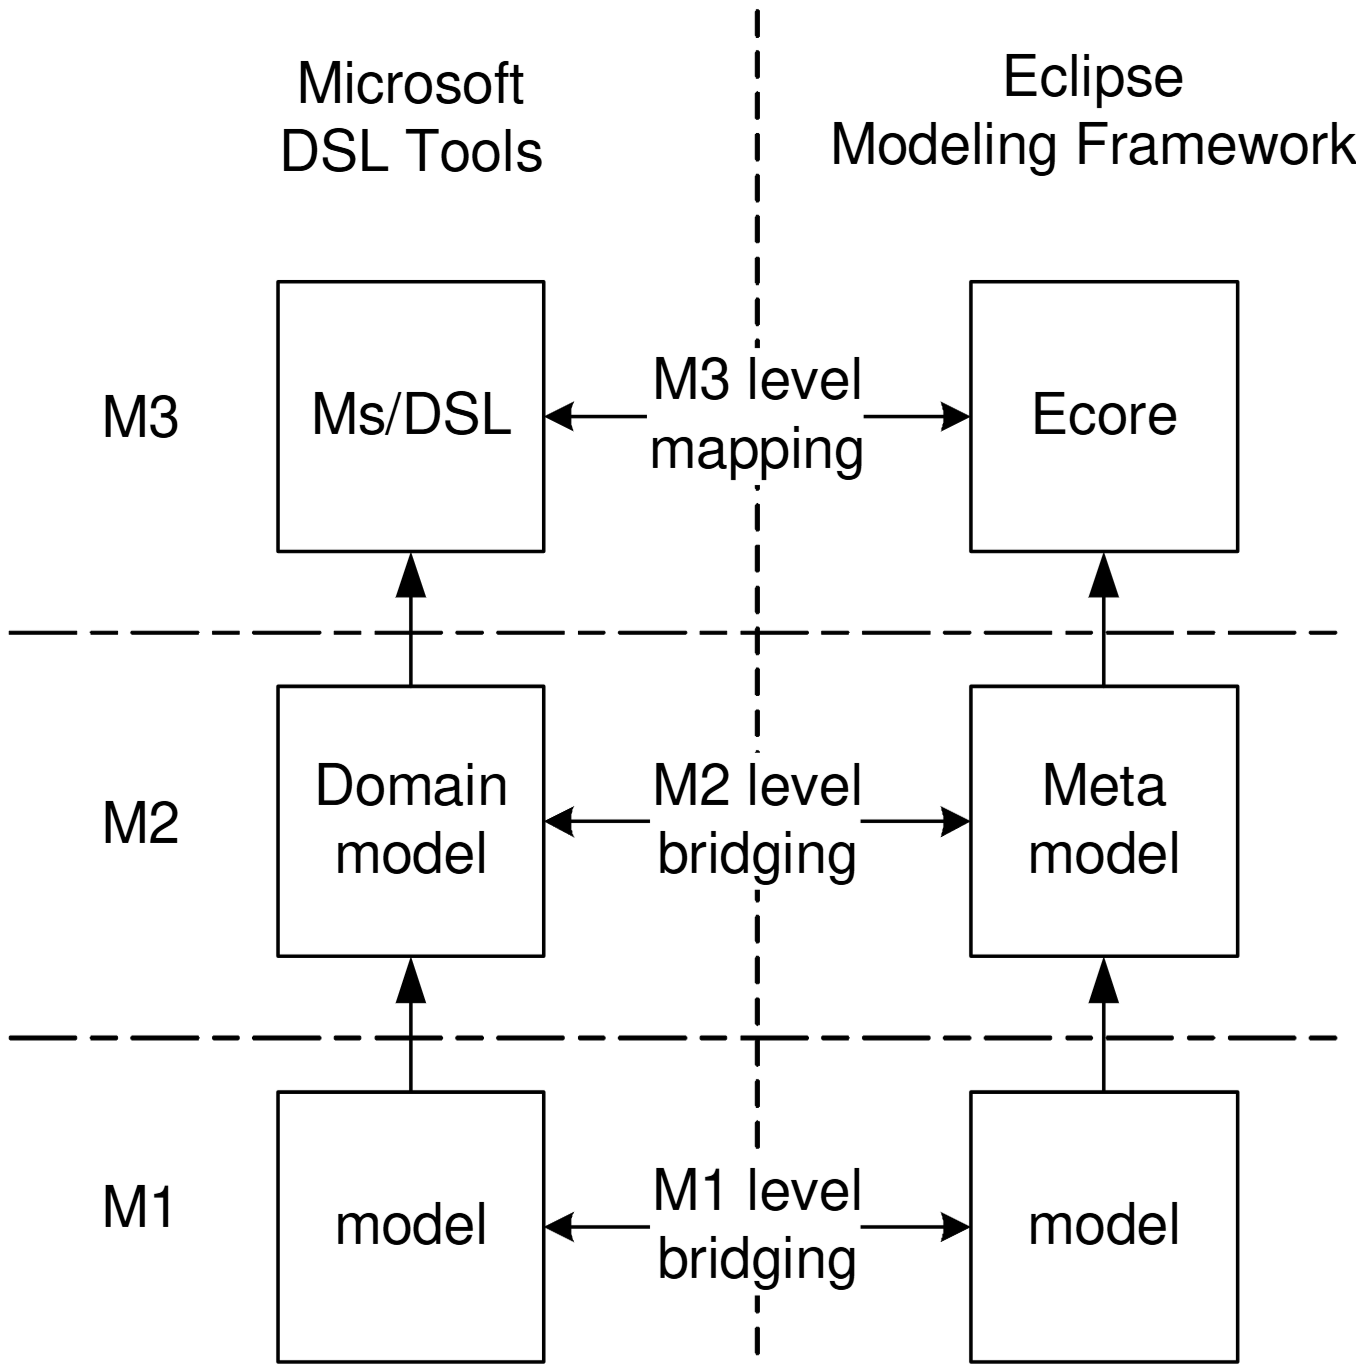
\includegraphics[width=.6\linewidth]{figures/emf-levels.png}
    \caption{Connection between model levels \cite{bezivin2005bridging}}
    \label{fig:emf-levels}
\end{figure}

M0 is not visible in \autoref{fig:emf-levels}.
This represents a real system without any kind of abstractions.
M1 is used for the first layer of abstraction representing models.
These models represent instances close to existing elements, such as Java code.
One level further, metamodels are defined.
A metamodel represents the world in which models live.
It provides a comprehensive definition of metaclasses.
It is evident that each element of a model on M1 is an instance of precisely one of them \cite{kuhne2006matters}.
Both UML and JaMoPP are examples of metamodels.
Consequently, a class in Java source code is therefore an instance of a metaclass defined by JaMoPP.
This principal finds equal application in the context of a class within a UML model, which constitutes an instance of a metaclass defined by UML \cite{heidenreich2009closing,bezivin2005bridging}.
The final level, M3, is referred to as the meta-metamodel.
This level defines the conceptual framework that is applicable for the definition of metamodels \cite{omgMof}.
In the context of EMF, Ecore assumes responsibility for this process.
It provides constructs such as \texttt{EClass}, \texttt{EAttribute}, and \texttt{EReference}, through which metamodels like UML or JaMoPP are expressed.
The presence of a meta-metamodel, defined in terms of itself, prevents the existence of any additional level of abstraction.
The Ecore model is the basis for the description of Ecore, thereby establishing that \texttt{EClass} is an instance of \texttt{EClass}.
An additional level would only repeat the concepts already present on M3 and is therefore omitted \cite{emfDocs,omgMof}.

Ecore facilitates the utilization of metamodels in the work.
It is possible to group each metamodel by its namespace URI with an \texttt{EPackage} stored in a global package registry.
\texttt{EClass} represents a metaclass capable of holding different structural features, like \texttt{EAttribute} or \texttt{EReference}.
The reference can be classified as either containment or non-containment.
It is shown that each object is limited to at most one \texttt{eContainer}, allowing the model to form a containment tree.
Roots have no container and sit directly in a resource.
The deletion of an object from its container also results in the removal of the subtree and the reference that points to it \cite{emfDocs}.

A notification is dispatched for each modification.
It carries the event type, the structural feature as well as both the old and new values.
The responsibility for receiving these notifications falls upon an \texttt{EContentAdapter} \cite{emfDocs}.

The persistence of models is an inherent feature of EMF.
A \texttt{Resource} represents a unit of persistence.
Addressing it works with URIs, and it gets saved and loaded as a whole.
The working context, which is responsible for loading resources and resolving references between them, is referred to as a \texttt{ResourceSet}.
A reference to an element in another resource is stored as a URI that identifies the target resource, together with a fragment identifying the element within it.
The ResourceSet resolves such a reference in a lazy manner, which means that the target resource is loaded only once the reference is accessed.
The process of resolution facilitates the conversion of a potentially logical URI into a physical one, thereby enabling the factory registry to select the parser for that particular resource.
\texttt{XMI} would be used for \texttt{.uml} files, while \texttt{JaMoPP} is utilized for \texttt{.java} files \cite{emfDocs,heidenreich2009closing}.
XMI is utilized for the purpose of serialization within the EMF framework.
In this approach, each resource is allocated to its own file.
It is important to note that the references contained within are URI fragments.
By default, these are positional paths depending on the order, but they can also be fixed \texttt{xmi:ids} \cite{omgXmi,emfDocs}.

\section{Vitruvius}
\label{sec:Foundations:Vitruvius}

One of the most important foundations for this thesis is Vitruvius itself.
Vitruvius is a framework for managing and keeping models consistent in a model-driven engineering context.
In a typical MDE system, different domain experts work with their own models, each describing a particular aspect of the same system.
Because all of these models describe different aspects of the same reality, they have overlapping information and must stay consistent with each other \cite{KLARE2021110815}.

One possible solution for keeping multiple models consistent is the view-based approach.
In theory, a Single Underlying Model (SUM) would contain all information about the system, and different views would simply project the relevant subset to each expert.
Often it is not feasible to have such a single monolithic model representing all aspects of a system, so Vitruvius introduces the concept of a V-SUM \cite{amrani2024survey,hermann2024towards}.
A V-SUM combines multiple independent models and exposes views to interact with them, giving the illusion of a single source of truth.
The process surrounding a V-SUM defines two distinct roles.
The methodologist is tasked with the creation of the V-SUM metamodel, a process that involves the selection of the involved metamodels, the establishment of the consistency preservation between them, and defining view types.
Consequently, the focus is on metamodel elements.
The developer utilizes the predefined views to create, access, and manipulate the V-SUM, without having the capability to modify the V-SUM metamodel itself \cite{KLARE2021110815}.

The consistency preservation mechanism in Vitruvius is based on Consistency Preservation Rules (CPRs).
A CPR specifies the requisite response to a particular change in a single model to restore consistency with related models.
The CPRs are specified using the Reactions Language, which provides the methodologist with a structured means of expressing these rules without resorting to general-purpose code \cite{KLARE2021110815}.
Reactions generate a set of \texttt{ChangePropagationSpecifications}, which are then employed to construct a V-SUM.
The remaining components necessary for the construction of a V-SUM include the metamodels themselves, a user interactor and a designated storage folder, where all data will be stored \cite{vitruviusGithub}.
One thing getting persisted are correspondences.
They function as an identifying link between elements from various models.
Reactions establish explicit correspondences and can be used to record which element was derived from which \cite{KLARE2021110815}.

Building upon the foundations laid out in \autoref{sec:Foundations:EMF}, atomic changes can be created by implementing an EContentAdapter to receive notifications.
Upon receiving a notification an atomic change is initiated, documenting a specific modification, such as the creation, deletion, insertion, removal or replacement of an element.
Changes are ordered within a \texttt{transactional change} \cite{KLARE2021110815}.

A view is defined as a copy of models in its own ResourceSet and edits are confined to the view's ResourceSet.
The two methods of capturing edits depend on its trait.
The conventional delta-based approach is employed for the purpose of recording change, whereby each EMF notification is transformed into an atomic change.
An alternative approach is to adopt a state-based model.
Upon the commit of a view, a comparison is started between its previous and current states, thereby deriving any alterations that occurred.
A commit transmits changes to the V-SUM itself, where they are implemented in its own models and subsequently transferred to specifications.
Those alter target models and correspondences, thereby introducing new changes \cite{KLARE2021110815,wittler2023evaluating}.

Even though Vitruvius' consistency preservation system typically operates automatically, there are some circumstances where manual intervention is still required.
An interactive dialog can be used to prompt the user when a reaction does not have enough information to determine how to proceed.
The user can choose between several options, accept or reject a transformation, or even enter custom data.
For instance, the framework may not be able to determine whether a new class in the source code represents a basic utility class or an architectural component.
In these situations, a dialog prompts the developer for clarification before carrying out the transformation \cite{vitruviusGithub}.
Although this mechanism increases flexibility, it also introduces runtime variability because the result is contingent upon the user.

\section{Reactions Language}
\label{sec:Foundations:ReactionsLanguage}

The Reactions language is an imperative DSL designed to work with provided delta events to keep models consistent.
It has two basic building blocks: Reactions and Routines.
Reactions are triggered through change events and will call the corresponding routines to perform the necessary repair actions on other models \cite{KLARE2021110815}.
Routines contain the actual logic to update the models.
They can call other routines or directly manipulate the models to achieve consistency.
A routine has three phases, which are \textit{match}, \textit{create} and \textit{update}.
In the match phase preconditions are checked to see if this routine is applicable for the given change and required resources are acquired.
One precondition is the check guard, which can test any arbitrary condition.
If the match phase is successful, the create phase will generate any new elements needed for the update.
Finally, the update phase will perform the actual routine calls and model manipulations to restore consistency in this model \cite{reactionsDocumentation}.
The language is implemented using Ecore and Xtext, which is a framework for developing DSLs in Eclipse.
The actual code can be written in Xtend, a statically typed programming language that compiles to Java source code, but offers some additional features to make the code more concise \cite{xtext,xtend}.
It is important to note that each Reaction has already been assigned a qualified name \cite{reactionsDocumentation}.
This is necessary for subsequent developments.

\section{JaMoPP}
\label{sec:Foundations:JaMoPP}

The Java Model Parser and Printer (JaMoPP) is an Ecore metamodel for Java as well as a parser and a printer.
The parsing of a given URI inside EMF is managed by the resource factory registered for the specific type.
JaMoPP has been identified as the primary resource factory for the \texttt{.java} domain.
The source code can be parsed into a model, and subsequently "printed" back as code.
This is a requisite, given that with the context of Java, source code assumes the role of the model file.
It is important to note that every element is regarded a compilation unit, including individual expressions.
In contrast to EMF, references are not stored as URIs.
These issues are resolved by a qualified name against a global classpath registry, which is not part of a single V-SUM.
A significant distinction between EMF and Java is the inability of Java elements to carry identifiers directly, as the source code lacks the capability to store them \cite{heidenreich2009closing}.

\section{Software Product Lines}
\label{sec:Foundations:SoftwareProductLines}

Software Product Lines (SPL) represent an evolution of traditional product lines into the digital domain.
SPL's area of expertise lies in the field of software artifacts, as opposed to physical products.
Those artifacts are derived from a shared set of software assets.
This facilitates the development of multiple software products that share common features, while still allowing for variability and customization \cite{clements2002software,bachmann2005variability}.
It happens in two distinct phases.
Domain engineering is concerned with the creation of assets and the variability, while application engineering is concerned with the derivation from these assets \cite{pohl2005software,apel2013software}.
In this thesis, the assets are the annotated reactions, which collectively form a 150\% model.
A configuration is defined as the set of selected features, and the product is the rule set derived from it, which reduces the 150\% model to a 100\% model \cite{kaestner2008granularity,czarnecki2005mapping}.

A feature is defined as a unit of variability, that serves to distinguish products from each other.
The generation of a configuration from a comprehensive array of features requires a set of guidelines on how to combine them.
It is evident that a feature model fulfils this purpose, by creating restrictions on combinations of different features.
The features contained within can be modelled as a tree with different group types.
\texttt{Mandatory} requires that every feature in the group be selected if the parent feature is selected.
The utilization of an optional group facilitates the selection of children, although this is not required.
For an \texttt{alternative}, it is necessary that exactly one of the children is selected, thereby representing an XOR relation \cite{van2001notion,kang1990feature}.
The ability to select at least one child is modelled by \texttt{or}.
Cross-tree constraints represent dependencies that cannot be modelled in any other way \cite{nevsic2019principles}.
The creation of a textual representation of a feature model is possible in \texttt{uvl}, which is the result of a community effort to establish a unified language for variability models \cite{uvl}.

A configuration that is deemed valid is one that satisfies the group types and all cross-tree constraints.
Validity may be regarded as a satisfiability check, a function performed by tools like Flamapy IDE \cite{white2010automated,flamapy-ide,kastner2009featureide}.
\chapter{Related Work}
\label{ch:RelatedWork}

In model-driven systems, consistency specifications are regarded as the stable component.
It is acknowledged that models may vary across products, the metamodels evolve over time, and existing artifacts are migrated whenever either models or metamodels change.
It is a commonly held assumption that the rules relating to the models remain applicable valid throughout course of the process.
In scenarios where variability is permitted within the rules themselves it is resolved prior to the existence of any artifacts.
Ensuring nothing derived from an earlier variant requires reconsideration.

\section{Variability in model transformations and consistency rules}
\label{sec:RelatedWork:VariabilityInModelTransformationsAndConsistencyRules}

In the context of model transformations research, variability has been identified as a contributing factor, mainly manifesting within the models themselves.
The rules are re-targeted or annotated to process a whole product line, yet they remain fixed.
In instances, where variability is introduced within the rules, it is resolved during the matching process or prior to compilation.
The subsequent papers do not ask of reconsidering the derived transformation.

Strüber et al. have developed a methodology for the integration of similar rules into a unified \texttt{variability-based rule} \cite{struber2018variability}.
Such a rule maintains the union of elements of all the rules it replaces, and parts where rules differ are guarded by presence conditions over variation points.
In the case of the common part, the match is computed only once and specialized per configuration afterward.
The variability is resolved during matching with one artifact representing all variants \cite{struber2018variability}.
The preprocessor described in this thesis resolves annotations earlier, resulting in conventional reactions for the V-SUM without any variability.

The closest architectural precedent extends the \textit{Atlas Transformation Language} (ATL) itself \cite{sijtema2010introducing}.
Sijtema incorporates a \texttt{variability rule} as a construct of the language, which is derived from the standard rule metaclass.
This approach preserves the declarative nature of the original and the implicit scheduling of a standard ATL rule.
Execution semantics are applied precisely when the corresponding variant is selected in the feature model.
It is important to note that this extension does not necessitate a modified engine.
A further transformation compiles the ATL with the new modification into a plain ATL model.
The engine is able to execute those functions, thereby eliminating the need for a plugin \cite{sijtema2010introducing}.
The same reasoning can be applied to annotated reactions.
These reactions are reduced to ordinary reactions prior to compilation, so neither the compiler of the Reactions Language nor Vitruvius needs any support for features.
ATL transformations are unidirectional and stateless.
Consequently, modifications to the variant selection necessitate the implementation of new transformations, which are applied to the source models again \cite{sijtema2010introducing}.
A V-SUM does not exhibit such behavior, given its persistence across iterations.
The paper does not address the artifacts that come from a variant change.
However, it is precisely these artifacts that motivate the migration developed in \autoref{sec:Concept:Migration}.

The expansion of Vitruvius to accommodate variability has been previously explored.
Ananieva et al. propose a unified conceptual model that incorporates variability in space and time.
The interrelated models of a variable system are maintained in a state of consistency as the system evolves.
CPRs form a fixed frame for that construction.
The fundamental system is the variable element in this context.
Consequently, the product line comprises models with a single rule set applicable to all models within the line \cite{ananieva2022preserving}.
In the present work the product line is assembled out of the rules, thereby establishing a complementary relationship between the two.

Neumann et al. integrate the consistency preservation mechanisms of Vitruvius with delta-oriented variability modelling \cite{neumann2025towards}.
A delta consists of operations that add, remove, or modify model elements. Applying a delta transforms one model variant into another.
Deltas are developed for a single domain and applied to a core model that remains consistent across all domains.
Within Vitruvius, applying a delta initiates changes that activate the consistency preservation rules.
The rules identify corresponding changes in other domains, which are then recorded as deltas specific to those domains.
This approach aligns with Vitruvius, as a delta represents a change and Vitruvius maintains consistency by propagating such changes.
Similar to the approach of Ananieva et al., the models exhibit variability, whereas the consistency preservation rules remain unchanged for each variant.
Future work aims to define consistency preservation rules between deltas rather than between metamodels, ensuring that modifications to variability also remain consistent \cite{neumann2025towards}.
This thesis addresses variability in the mapping between metamodels, such as determining whether a UML class is mapped to a Java class or a Java interface.
Such a mapping is defined by the consistency preservation rules, so a delta applied to a model cannot vary it.

\section{Annotative variability}
\label{sec:RelatedWork:AnnotativeVariability}

Annotative variability marks the elements of an artifact directly with the features they belong to \cite{kaestner2008granularity}.
Sulír et al. attach a concern adjacent to the element to which it belongs.
The intent behind a piece of code is embedded within the code itself, rather than being conveyed through a separate document.
Those concerns merely document, rather than derive, as no variant is selected from them.
The mechanism outlined in this thesis employs locality, yet the preprocessor functions by reading reactions and determining which elements get kept \cite{sulir2016recording}.

\section{Migration of existing artifacts}
\label{sec:RelatedWork:MigrationOfExistingArtifacts}

The migration of artifacts whose definition has undergone modifications is a recognized issue, provided that the definition in question is a metamodel.
In the implementation in this thesis, the metamodels are untouched, and the models maintain their validity.
The underlying specifications undergo alterations, resulting in the disruption of correspondence.

In Hearnden et al., the transformation is maintained in a running state and the derivation of each component of the target is recorded \cite{hearnden2006incremental}.
A change can be mapped onto the target incrementally instead of doing everything at once again.
The authors argue that the same mechanism can be applied to a change of the transformation definition itself, rendering it the closest published work to the problem covered in this thesis.
The record is the memory context, while a V-SUM is persisted between runs.
The changed rules have to be recovered afterward from identifiers, hashes and triggers.

Leonhardt et al. commence their investigation by assuming the same observation, relying on changes that have been recorded \cite{leonhardt2015integration}.
A strategy that is employed involves the synthesis of the change sequence that would have generated the models and propagated it afterward.
That represents the internal replay used in \autoref{sec:Concept:Migration}.
Given that the artifacts were built outside Vitruvius, no existing V-SUM, including correspondences is available.
They have to start from an empty V-SUM with a predefined rule \cite{leonhardt2015integration}.
In the thesis correspondences already exist and only the underlying rules change.

\section{Preservation of handwritten content}
\label{sec:RelatedWork:PreservationOfHandwrittenContent}

Greifenberg et al. have conducted a comparative analysis of eight mechanisms that integrate handwritten and generated code, including partial classes and protected regions \cite{greifenberg2015integration}.
Each of them fixes the place where handwritten code may appear in advance.
Vitruvius does not fix such place.
An element no correspondence points at counts as underived.
Everything the rules did not derive ends up in the preservation report (\autoref{sec:Concept:Migration:Preservation}), whether a person wrote it or not.

\section{Other consistency approaches}
\label{sec:RelatedWork:OtherConsistencyApproaches}

Alternative approaches to maintaining consistency in models utilize mechanisms that are not connected to the Reactions language.
Each of these systems operates under the assumption that its own specification is given.
Multi-version models enable the storage of a model's history within a single graph.
This property of multi-version models facilitates transformations that can operate on multiple versions concurrently.
Barkowsky and Giese employ triple graph grammars to define such transformations on multi-version models.
The simultaneous transformation of all versions reduces memory usage and can reduce execution time for extensive version histories.
However, it can add overhead in less favorable circumstances \cite{barkowsky2023incremental}.
It is important to note that reactions utilize the current version of a model exclusively and possess no history.
Graph stores are designed to host versions of the models rather than the rules that relate to them.

König et al. express the correspondence as a query.
The relational operators define views over the models and each of them is consolidated into a triple graph rule.
Those views are analogous to queries in relational databases.
The transformation and synchronization of these views is then managed by the grammars.
In this approach, operators are not regarded as entities that undergo change \cite{konig2025transforming}.

\section{Research gap}
\label{sec:RelatedWork:ResearchGap}

Variability in model transformations exists, but it gets resolved before any artifact is derived from it \cite{struber2018variability,sijtema2010introducing}.
Inside Vitruvius the variability is carried by the models, while the reactions relating them remain fixed \cite{ananieva2022preserving,neumann2025towards}.
The migrating of artifacts whose definition has undergone modification is also well-defined, provided that the definition in question is a metamodel.
Incremental re-execution after a change of the transformation itself was found only once, assuming an engine that keeps running.
The authors argue for this extension rather than providing a demonstration of it \cite{hearnden2006incremental}.
Vitruvius has the capability to incorporate existing artifacts into an empty V-SUM, but with reactions that do not change \cite{leonhardt2015integration}.
Alternative approaches to consistency treat their own specification as a given \cite{barkowsky2023incremental,konig2025transforming}.
A proposal within Vitruvius aims to establish consistency preservation rules between deltas rather than between metamodels.
Its variants start from a consistent core model and are derived under rules that do not change \cite{neumann2025towards}.
No publication was found that altered the consistency specification of a previously recorded V-SUM, which is the gap this thesis addresses.
\chapter{Running Example}
\label{ch:RunningExample}

The case study umljava provided in \cite{umljavacasestudy} serves as the running example.
It contains basic reactions code for preserving consistency in both directions, providing a good baseline for further expansion.
In addition to the reactions, the library example provides models of the real V-SUM that were used for testing and measurements.

\section{Reactions}
\label{sec:RunningExample:Reactions}

The first thing to consider is the actual reaction code and what can be built upon.
Existing reactions have been altered throughout this work by adding and adapting rules to fit the needs of derived configurations.

\lstinputlisting[frame=single, caption={Existing UML to Java reaction}, label=listing:existing-reaction, numbers=left, float=htbp, language=reactions]{examples/umlClassInserted.reactions}

\Autoref{listing:existing-reaction} shows an existing reaction that is responsible for creating or locating an existing Java class and connecting it to the newly created UML class.
Line one defines a new reaction called \textit{UmlClassInserted}.
The next line adds the trigger for this reaction, which starts the procedure when a new UML class is inserted.
The routines to execute are defined in the \textit{call} block and will be called when the reaction is triggered.

\lstinputlisting[frame=single, caption={Existing UML to Java routine}, label=listing:existing-routine, numbers=left, float=htbp, language=reactions]{examples/createOrFindJavaClass.reactions}

The routine definition for \textit{createOrFindJavaClass} is given in \autoref{listing:existing-routine}, which executes the actual logic with the help of Xtend code \cite{KLARE2021110815}.
The \textit{match} block ensures that this routine can be run, as it requires the absence of an existing Java class already linked to the UML class.
It also retrieves the optional Java package corresponding to the UML container in lines 4 \& 5.
This is used in the \textit{update} block, which can contain arbitrary Xtend code for creating files, changing packages, adding attributes, and so on.
This code can also call other routines and functions defined in Java.

\lstinputlisting[frame=single, caption={Routine calling a user interaction}, label=listing:external-method-call, numbers=left, float=htbp, language=reactions]{examples/propagateTypedMultiplicityElementTypeChanged.reactions}
\lstinputlisting[frame=single, caption={Existing user interaction}, label=listing:existing-user-interaction, numbers=left, float=htbp, language=Java]{examples/userSelectCollectionType.java}

One important functionality that remains to be examined is user interaction.
When a reaction has code for user interaction, the user is prompted with one of the possible dialogs, which they must complete to continue execution.
\Autoref{listing:external-method-call} is a routine that calls into code defined in Java, presenting the user with an interactive option.
In \autoref{listing:existing-user-interaction}, the user is asked what type of collection should be used on the Java side when the multiplicity on the UML side changes.
The result can then be used like any other variable in the code.
Expressing such a dialog in terms of features is left to \autoref{ch:FutureWork}.
Currently, the annotated reactions still contain it, so it remains a runtime decision in every derived configuration.
For now, a predefined selection is used, with the first option chosen in automatic runs.

Further reactions need to be added to enable variability and allow annotations to choose which features to use.
If a new UML class is to be modelled as a Java interface, the methodologist must create this new reaction, which can then be selected by the annotation representing the feature.
The case study also includes tests written in xtend to verify the behavior of its reactions.
These are extended to cover the new features and configurations, as described in \autoref{sec:Implementation:Testing}.

\section{Features and configurations}
\label{sec:RunningExample:FeaturesAndConfigurations}

One of the created artifacts is a feature model that defines the relationship between all features.
This is necessary so that the methodologist knows which configurations are valid.
The full model contains 37 features.

\begin{sidewaysfigure}
    \centering
    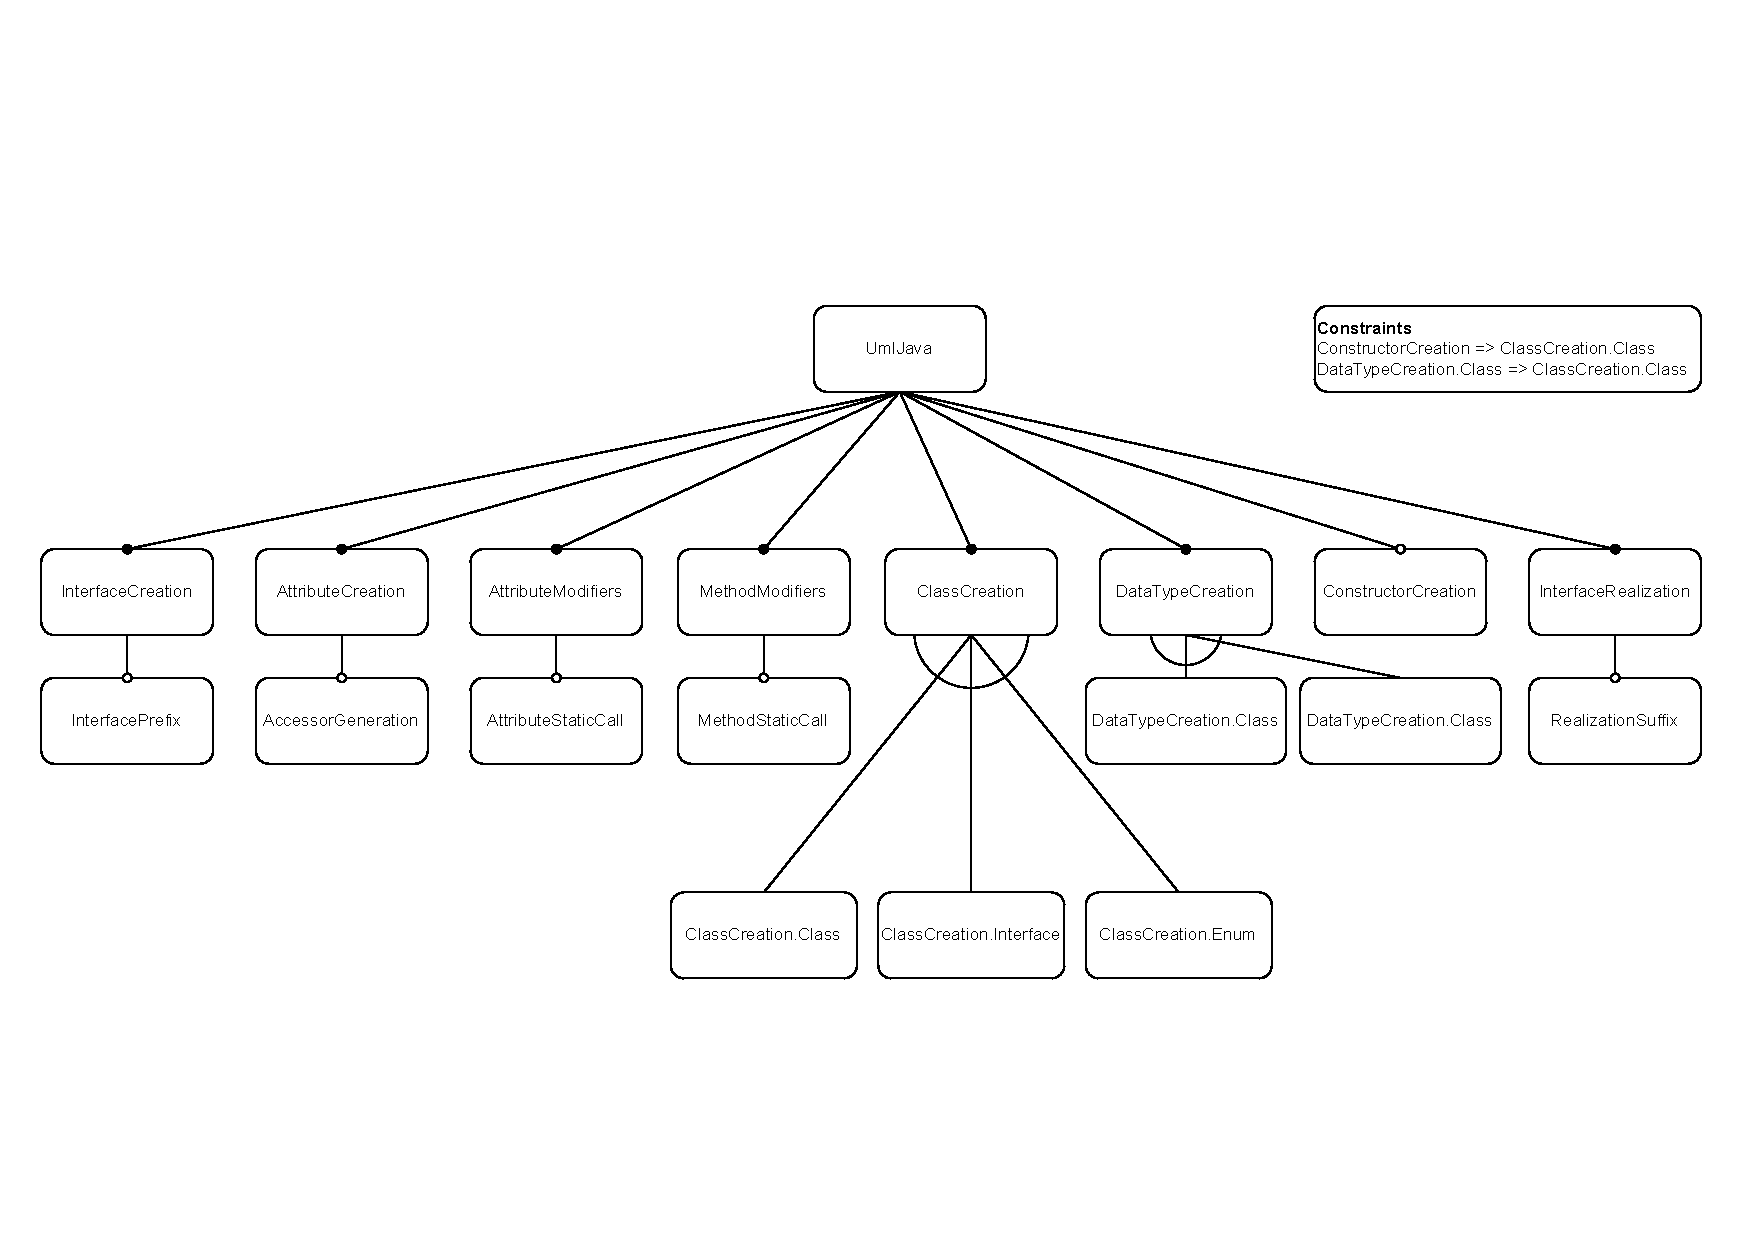
\includegraphics[width=\textheight, height=0.9\textwidth, keepaspectratio]{examples/library/reduced feature model.pdf}
    \caption{Reduced feature model}
    \label{fig:reduced-feature-model}
\end{sidewaysfigure}

Only a small subset is shown in \autoref{fig:reduced-feature-model}.
The excluded features are either mandatory or appear in every configuration, so it is not necessary to examine them more closely.
With the help of the feature model, nine configurations are extracted to represent all features at least once.
This allows each feature to be tested on its own.

\begin{table}[htbp]
    \centering
    \begin{tabular}{|l|c|c|c|c|c|c|c|c|c|}
        \hline
        \textbf{Feature}                 & \textbf{1} & \textbf{2} & \textbf{3} & \textbf{4} & \textbf{5} & \textbf{6} & \textbf{7} & \textbf{8} & \textbf{9} \\
        \hline
        \textit{Feature core}            & \checkmark & \checkmark & \checkmark & \checkmark & \checkmark & \checkmark & \checkmark & \checkmark & \checkmark \\
        \hline
        \textit{ClassCreation.Class}     & \checkmark & \checkmark & \checkmark & \checkmark & \checkmark & \checkmark &            &            & \checkmark \\
        \hline
        \textit{ClassCreation.Interface} &            &            &            &            &            &            & \checkmark &            &            \\
        \hline
        \textit{ClassCreation.Enum}      &            &            &            &            &            &            &            & \checkmark &            \\
        \hline
        \textit{DataTypeCreation.Class}  & \checkmark & \checkmark & \checkmark & \checkmark & \checkmark & \checkmark &            &            & \checkmark \\
        \hline
        \textit{DataTypeCreation.Record} &            &            &            &            &            &            & \checkmark & \checkmark &            \\
        \hline
        \textit{InterfacePrefix}         &            & \checkmark &            &            &            &            &            &            & \checkmark \\
        \hline
        \textit{RealizationSuffix}       &            &            &            & \checkmark &            &            &            &            & \checkmark \\
        \hline
        \textit{AccessorGeneration}      &            &            & \checkmark &            &            &            &            &            & \checkmark \\
        \hline
        \textit{ConstructorCreation}     &            &            &            &            & \checkmark &            &            &            & \checkmark \\
        \hline
        \textit{AttributeStaticCall}     &            &            &            &            &            & \checkmark &            &            & \checkmark \\
        \hline
        \textit{MethodStaticCall}        &            &            &            &            &            & \checkmark &            &            & \checkmark \\
        \hline
    \end{tabular}
    \caption{Features selected by the nine configurations. A checkmark marks a selected feature, and the feature core row stands for the 26 features every configuration selects.}
    \label{table:library-configurations}
\end{table}

\Autoref{table:library-configurations} lists the selected features by each of the nine configurations.
26 of the 37 features are selected in every configuration and form the core mapping between UML and Java.
These features cover the mapping of models, packages, names, visibilities, multiplicities, and primitive types, the creation and deletion of classes, attributes and methods, the creation of interfaces and enumerations, attributes, return and parameter types together with the direction of parameters.
They also cover class, attribute, and method modifiers, as well as inheritance, interface realization and the constraints of classes, interfaces, enumerations and parameters.
Like every other reaction, their reactions carry an annotation.
22 of these features are mandatory, so no valid configuration can drop them, whereas the four constraint features are optional but selected by all nine configurations.
Therefore, only the reactions of the remaining eleven features differ between two of the nine configurations.
Of those eleven features, only some are selected in each configuration.
\textit{ClassCreation} and \textit{DataTypeCreation} are alternative groups, so each configuration selects one of each, while the other features are optional.

The features from \autoref{fig:reduced-feature-model} have greater importance and require more information.
Their effects are shown in the classifiers of the library example in \autoref{sec:RunningExample:LibraryExample}, whose UML model is shown in \autoref{fig:library-example}.
\textit{InterfaceCreation} maps a UML interface to a Java interface in its own compilation unit, and vice versa.
Its optional child, \textit{InterfacePrefix}, prefixes the name of every interface with an \texttt{I} in both models, so \texttt{Borrowable} becomes \texttt{IBorrowable}.
Names starting with an \texttt{I} keep their original form, leaving \texttt{Identifiable} untouched.
\textit{AttributeCreation} maps UML properties to Java fields and vice versa.
With \textit{AccessorGeneration}, every attribute is made private and receives a getter and a setter.
These are renamed and deleted together with the attribute.
This turns \texttt{Media.title} into a private field with \texttt{getTitle} and \texttt{setTitle}.
\textit{AttributeModifiers} synchronizes the \texttt{final} and \texttt{static} modifiers of Java fields with the read only and static properties of UML attributes.
\textit{AttributeStaticCall} builds on that.
As soon as an attribute becomes static, its accessors become static as well.
Every access is rewritten as static access through the class.
Thus, the accessors of \texttt{LibraryCard.cardNumber} read and write \texttt{LibraryCard.cardNumber} instead of \texttt{this.cardNumber}.
Similarly, \textit{MethodModifiers} synchronizes the \texttt{abstract}, \texttt{final}, and \texttt{static} modifiers of Java methods with the abstract, leaf and static properties of UML operations.
Its optional child, \textit{MethodStaticCall}, works similarly to \textit{AttributeStaticCall}.
Furthermore, it turns the method \texttt{final}, which is a leaf operation in UML.
Consequently, the static \texttt{Member.register} becomes \texttt{static final}.
The function of \textit{ClassCreation.Class}, is to facilitate the mapping of a UML class to a Java class, and vice versa, in a manner consistent with the original reactions.
The new alternatives \textit{ClassCreation.Interface} and \textit{ClassCreation.Enum} realize every UML class as a Java interface or enum and every Java class as a UML interface or enumeration.
In the library example \texttt{Member} becomes an interface, with its attributes being designated as \texttt{static final} fields, or an enumeration without any literal.
\textit{DataTypeCreation.Class} maps a UML data type to a Java class, while the \textit{DataTypeCreation.Record} maps to a \texttt{final} Java class.
A final Java class is not extendable, a limit that also applies to \texttt{Isbn}.
It is not possible to establish a direct mapping to a Java record, as this functionality is not supported by \hyperref[sec:Foundations:JaMoPP]{JaMoPP}.
The \textit{InterfaceRealization} feature maps the interface realizations of UML classes to the \texttt{implements} references of Java classes, whenever one is added, removed, or replaced.
The optional child \textit{RealizationSuffix} functions similar to \textit{InterfacePrefix}, yet it appends \texttt{Impl} to a realization.
Consequently \texttt{Media} becomes \texttt{MediaImpl}.
Besides the four constraint features, the only optional feature located directly beneath the root element is \textit{ConstructorCreation}.
A public default constructor is appended to each new class, as an operation in UML and a constructor in Java.
The constructor is renamed, along with the class, resulting in the addition of a \texttt{Member()} constructor in \texttt{Member}.
The feature model introduces two additional constraints.
\textit{ConstructorCreation} and \textit{DataTypeCreation.Class} both require \textit{ClassCreation.Class}.

\section{Library example}
\label{sec:RunningExample:LibraryExample}

The process of obtaining measurements and the creation and interaction with a V-SUM necessitate a real example.
For the purpose of this study umljava is defined as a system that incorporates both a UML model and Java source code.
This integration enables the creation of a V-SUM with preprocessed reactions and can be migrated to different configurations afterward.
The example under consideration is a library with different types of media, interfaces with polymorphism, members, and all kinds of properties.
It is derived with the first configuration, which mirrors the behavior of the original reaction set.
The UML model for the first configuration is shown in \autoref{fig:library-example}.

\begin{figure}[htbp]
    \caption{Library example}
    \centering
    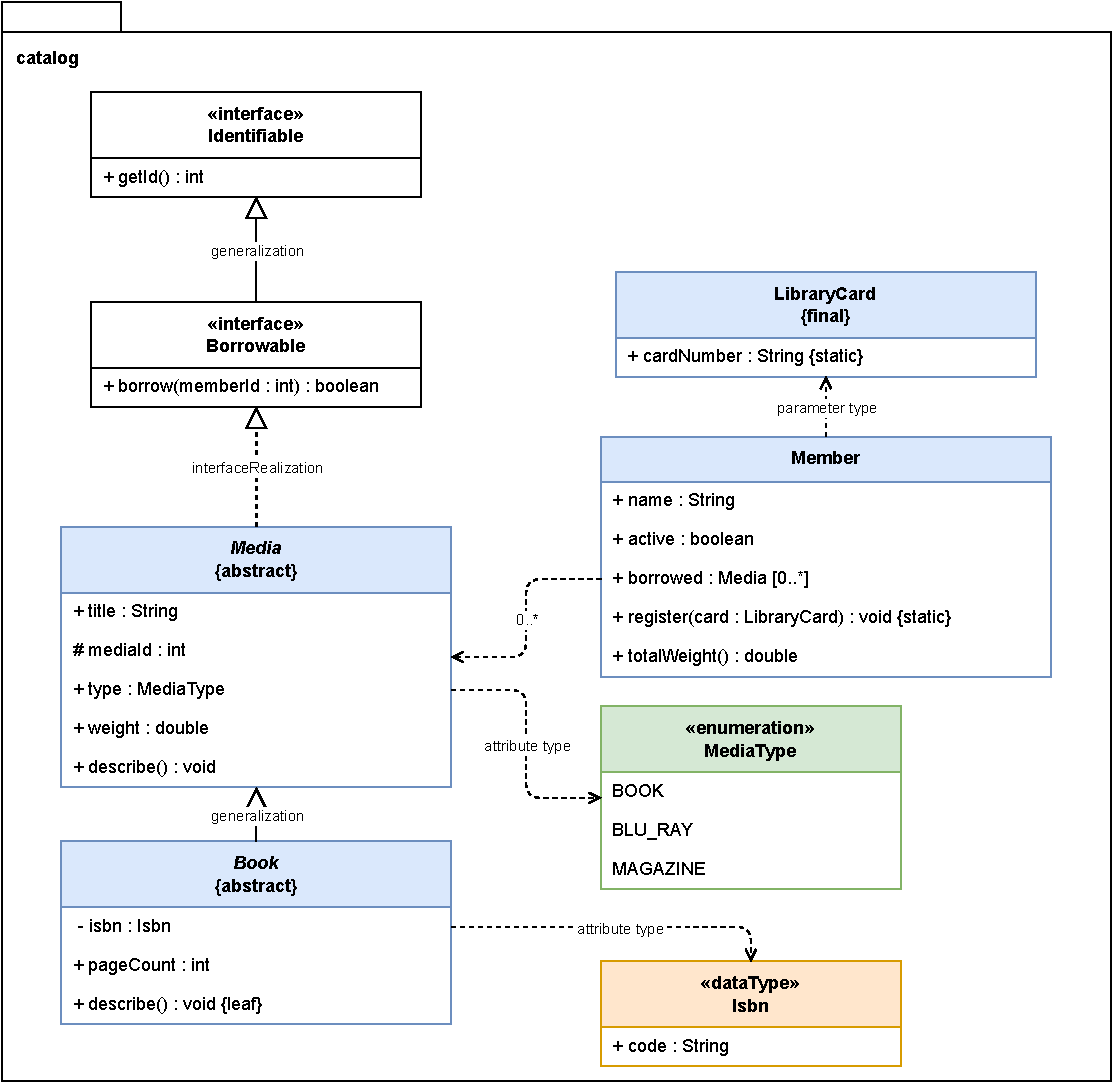
\includegraphics[width=\textwidth]{examples/library/library.pdf}
    \label{fig:library-example}
\end{figure}

All elements are contained within a single package \texttt{catalog} and consist of eight classifiers.
The interfaces \texttt{Identifiable} and \texttt{Borrowable}, the latter extends the former, and both declare the operations \texttt{getId} and \texttt{borrow}.
\texttt{MediaType} is an enumeration comprised of the literals \texttt{BOOK}, \texttt{BLU\_RAY} and \texttt{MAGAZINE}, while the \texttt{Isbn} data type is characterized by a single attribute \texttt{code}.
The abstract class \texttt{Media} carries the attributes \texttt{title}, the protected \texttt{mediaId}, \texttt{type} and \texttt{weight}.
It realizes \texttt{Borrowable} and declares \texttt{describe}.
The abstract \texttt{Book} extends it, and adds the private \texttt{isbn} and \texttt{pageCount}, in addition to a leaf \texttt{describe}.
\texttt{LibraryCard} is a final specialization holding the static \texttt{cardNumber}.
\texttt{Member} has the attributes \texttt{name}, \texttt{active} and \texttt{borrowed}, which holds zero to many \texttt{Media}, as well as the static operation \texttt{register} and the operation \texttt{totalWeight}.
Depending on the configuration that is selected, the V-SUM can accomodate between 216 and 437 model elements.
The least number of classifiers is observed in the seventh configuration, where classifiers become interfaces, that do not carry fields, accessors, or constructors.
The greatest number of classifiers is observed in the eighth and ninth configuration.

\lstinputlisting[frame=single, caption={Handwritten method body of \texttt{Member}}, label=listing:total-weight, numbers=left, float=htbp, language=Java]{examples/totalWeight.java}

While the rules derive the attribute \texttt{Media.weight} and the signature of \texttt{Member.totalWeight} from the UML model, the body shown in \autoref{listing:total-weight} has no counterpart there.
The method is composed of three statements, a local variable declaration, a loop over the borrowed media accumulating their weight, and a return.
This constitutes the sole instance of user written content in the given example, which serves as one criterion for evaluating the preservation of such content.
\chapter{Concept}
\label{ch:Concept}

A methodologist first annotates the reactions of a consistency specification with the features they belong to.
A derivation step then reduces the annotated specification to the rules of a single configuration.
Everything built with those rules is consistent under them, whereas a V-SUM that was persisted under an earlier configuration is not.
The second part of the chapter therefore describes the migration that brings such a V-SUM to the rules it is loaded with.
The feature model, the nine configurations and the library example are introduced in \autoref{ch:RunningExample}.
The approach is stated independently of the tool that realizes it and of the metamodels it is applied to, a claim that \textbf{M5.1} and \textbf{M5.2} put to the test.
The realization is described in \autoref{ch:Implementation}, and \autoref{ch:Evaluation} reports the measurements defined by the metrics of \autoref{sec:Introduction:ResearchGoals}.
Each part of this chapter names the metrics that judge it.

\section{Feature annotations}
\label{sec:Concept:FeatureAnnotations}

A consistency specification written in the Reactions Language fixes one mapping between the involved metamodels.
Several mappings are often defensible.
A UML class can be realized as a Java class, as an interface or as an enumeration, and the methodologist has to commit to one of these alternatives.
Supporting a second project convention then requires a second copy of the specification, in which every correction to a shared rule has to be applied again.
Treating the specification as the asset base of a software product line removes that commitment, as described in \autoref{sec:Foundations:SoftwareProductLines}.
The reactions of all variants form one 150\% rule set.
Every reaction of that rule set carries an annotation with the feature it belongs to, which makes the variability annotative \cite{kaestner2008granularity}.
A feature model states which combinations of features are valid, whereas a configuration selects the rules of one variant \cite{apel2013software,czarnecki2005mapping}.
\textbf{M1.2} counts the files that an added or changed variant costs under either arrangement.

\subsection{Annotating reactions}
\label{sec:Concept:FeatureAnnotations:AnnotatingReactions}

An annotation is attached to a reaction and names the feature the reaction belongs to.
The reaction in \autoref{listing:annotated-reaction} realizes an inserted UML class as a Java interface.
It belongs to \textit{ClassCreation.Interface}, one of the three alternatives of \textit{ClassCreation}, and replaces \autoref{listing:existing-reaction} of the running example, which belongs to \textit{ClassCreation.Class}.
The feature names are those of the feature model in \autoref{sec:RunningExample:FeaturesAndConfigurations}, although the annotation does not check that the name it carries exists there.

\lstinputlisting[frame=single, caption={Reaction annotated with a feature}, label=listing:annotated-reaction, numbers=left, float=htbp, language=reactions]{examples/umlClassInsertedAnnotation.reactions}

An annotation carries exactly one feature name and admits neither boolean expressions over features nor nesting.
The restriction costs no expressiveness, because behavior shared by two features is expressed by a routine that the reactions of both features call.
A conjunction of features would merely restate in the asset base what the feature model already declares.
Routines carry no annotation at all.
Since they have no trigger, they belong to a feature only through the reactions that reach them, which is the property the derivation described in \autoref{sec:Concept:FeatureAnnotations:RuleSetDerivation} relies on.

\lstinputlisting[frame=single, caption={Routine selected by \textit{ClassCreation.Interface}}, label=listing:chosen-routine, numbers=left, float=htbp, language=reactions]{examples/createJavaInterfaceFromClass.reactions}
\lstinputlisting[frame=single, caption={Routine selected by \textit{ClassCreation.Enum}}, label=listing:possible-routine, numbers=left, float=htbp, language=reactions]{examples/createJavaEnumFromClass.reactions}

The two alternatives of \textit{ClassCreation} differ in the routine their reactions call.
The routine in \autoref{listing:chosen-routine} creates a Java interface and is reached only through the reaction of \autoref{listing:annotated-reaction}.
The routine in \autoref{listing:possible-routine}, by contrast, creates an enumeration and is reached only through the corresponding reaction of \textit{ClassCreation.Enum}.
Both routines establish a correspondence between the UML class and the Java classifier they create.
That correspondence is the record of the derivation which the migration later reads.
\textbf{M1.3} records how much of the original rule set had to be changed to become a 150\% rule set.

\subsection{Rule set derivation}
\label{sec:Concept:FeatureAnnotations:RuleSetDerivation}

The derivation takes the 150\% rule set and one configuration and writes the rules of that configuration.
A reaction is kept if the configuration selects the feature its annotation names.
A reaction without an annotation belongs to no feature and could never be selected, so carrying one is a well-formed condition on a 150\% rule set rather than a consequence of the derivation.
The routines a reaction calls are kept with it, together with the routines those call in turn, whereas what no kept reaction reaches is left out.
This is how the routines of an unselected alternative disappear, although no annotation ever mentioned them.

Features that the feature model declares mandatory are part of every valid configuration, and their reactions appear in every derived rule set.
Only the reactions of the optional features and of the alternative groups differ between two configurations.
Two derived rule sets of the library example therefore overlap in the large majority of their rules.
The result of a derivation is an ordinary rule set without annotations.
Since the compiler of the Reactions Language processes it like any handwritten one, nothing downstream of the derivation has to know that features exist.
The derivation of config1 and config7 of the library example from the same 150\% rule set is shown in \autoref{fig:preprocessor-flow}.

\begin{figure}[htbp]
    \centering
    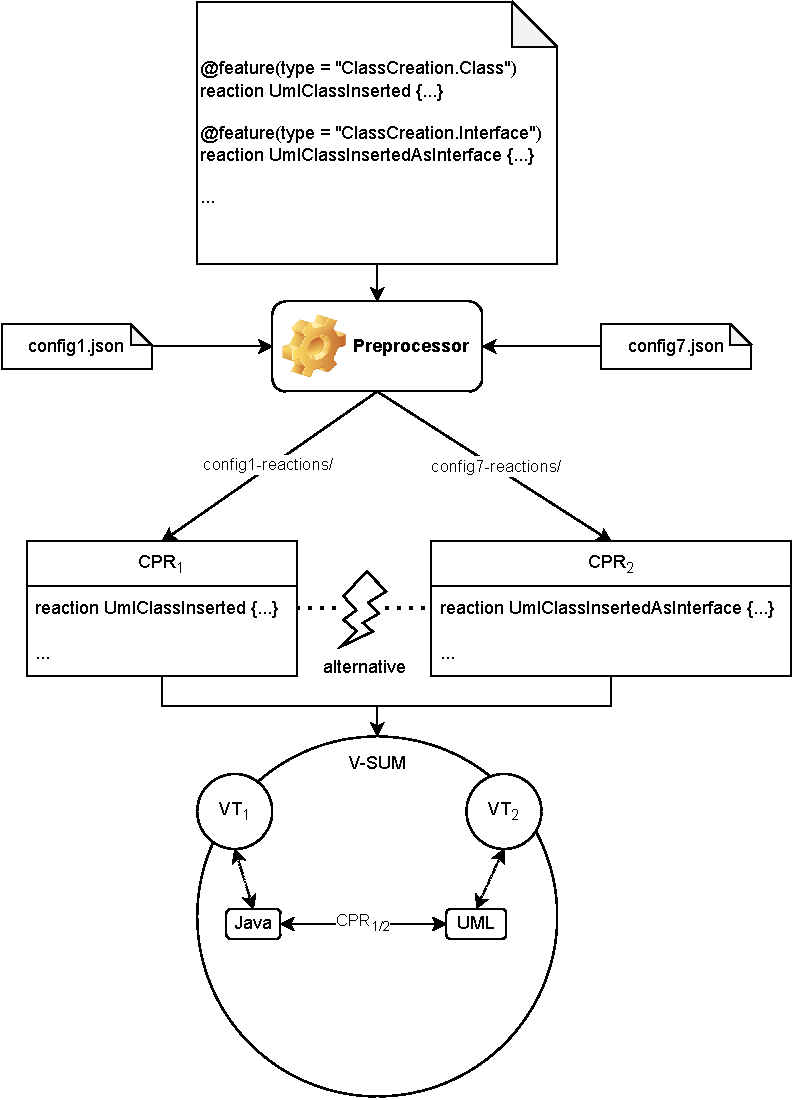
\includegraphics[width=\linewidth,height=0.85\textheight,keepaspectratio]{examples/library/preprocessor.pdf}
    \caption{Derivation of the configurations config1 and config7 of the library example from the annotated reactions.}
    \label{fig:preprocessor-flow}
\end{figure}

The derivation does not check the configuration it is given.
A configuration that violates the feature model by selecting two alternatives of \textit{ClassCreation} yields a rule set with two reactions on the same trigger rather than an error.
Ensuring validity is therefore a duty of the methodologist, who has the feature model to check a configuration against.

One property of the annotation matters beyond this section.
The annotation is not part of the abstract syntax of a reaction, and a kept reaction is written out unchanged apart from the annotation itself.
Two configurations therefore differ in which rules exist, never in what a rule they share does.
That property is taken up again in \autoref{sec:Concept:Migration:SelectiveMigration:SemanticHashes}.
\textbf{M1.1} compares the size of the 150\% rule set against the sum of the configurations it replaces.
\textbf{M1.4} checks that every derived configuration produces compilable code and passes the tests of the case study, whereas \textbf{M1.5} measures what the derivation adds to building and testing a configuration.

\subsection{Binding time}
\label{sec:Concept:FeatureAnnotations:BindingTime}

A feature annotation binds a decision when the rule set is derived.
Vitruvius already contains a second kind of variability, which binds later.
A reaction that lacks the information to proceed can ask the developer at runtime, as described in \autoref{sec:Foundations:Vitruvius}.
Both kinds produce several possible outcomes for one change, yet they do so at different moments and at a different granularity.
A configuration decides once for a whole rule set and is recorded in a file, whereas a dialog decides per element and can be answered differently in two runs of the same rule set.
Only the first of the two makes a run reproducible.

The running example contains such a dialog.
The collection type a Java field receives when the upper multiplicity of a UML property changes is chosen by the developer, as shown in \autoref{listing:existing-user-interaction}.
This work does not express that choice as a feature, so the dialog is present in the 150\% rule set and in all nine derived configurations.
A derived rule set is consequently free of compile-time variability but not of runtime decisions.
A migration has to answer such a dialog without a person present.
It records the interactions a run requires and supplies a fixed answer to each of them.
A question that cannot be answered safely aborts the run, so that no migration rests on an answer that was never given.
What moving such a decision to derivation time would require is discussed in \autoref{ch:FutureWork}.

\section{Migration}
\label{sec:Concept:Migration}

A derived rule set keeps a V-SUM consistent that is built with it.
A V-SUM that already exists was built with a different rule set, and nothing in it records that fact.
A persisted V-SUM holds its models, the correspondences between their elements and the identifiers of those elements, yet it holds no information about the rules that produced any of it \cite{vitruviusGithub}.
Loading it with a new rule set therefore succeeds and leaves the state untouched.
Only the changes made from that point on are propagated by the new rules.
Everything the old rules derived stays as it is, whether the new rules would derive it or not.
The result is a V-SUM that is consistent under neither rule set.
\textbf{M3.1} classifies the inconsistencies that arise in this situation.

Migration closes that gap.
It takes a persisted V-SUM and a rule set and leaves a V-SUM that is consistent under the rules it was given, keeping as much of the existing state as those rules allow.
Two ways of doing so are described here.
The full migration of \autoref{sec:Concept:Migration:FullMigration} keeps one model and derives everything else from it again, without asking what changed in the rule set.
The selective migration of \autoref{sec:Concept:Migration:SelectiveMigration} first establishes which rules changed and then restricts the work to the elements those rules apply to.
Since both leave behind content that no rule derives, the preservation step of \autoref{sec:Concept:Migration:Preservation} collects that content afterward.
\textbf{M2.1} compares a migrated V-SUM against the state the new rules derive from scratch.
\textbf{M2.2} checks that the migrated code still compiles, and \textbf{M2.4} whether migrating back reproduces the original V-SUM.

\subsection{Full migration}
\label{sec:Concept:Migration:FullMigration}

The full migration rests on the single assumption that one model of the V-SUM is authoritative and that every other model can be produced from it.
That model is the dominant model, whereas the models produced from it are the derived models.
Which model dominates is the only decision the full migration makes, and the three ways of making it are described below.
The procedure and those three strategies are shown in \autoref{fig:full-migration}.

\begin{figure}[htbp]
    \centering
    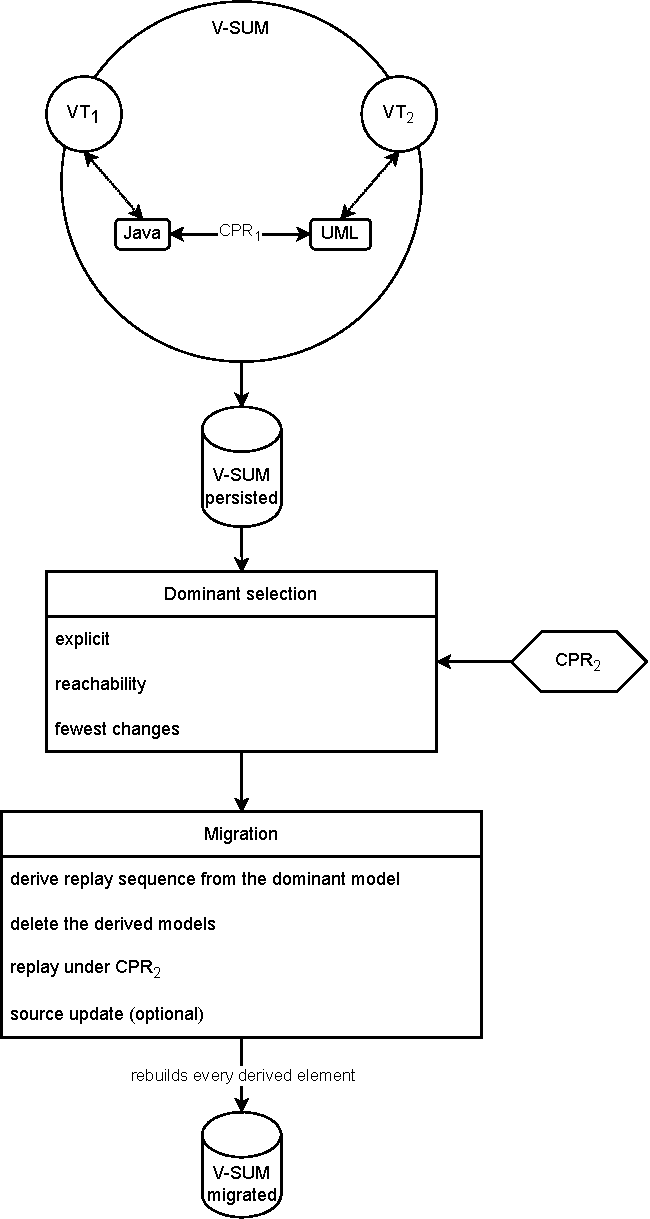
\includegraphics[width=\linewidth,height=0.85\textheight,keepaspectratio]{examples/library/migration.pdf}
    \caption{Full migration of a persisted V-SUM, from the selection of the dominant model to the derivation of the remaining models under the new rules.}
    \label{fig:full-migration}
\end{figure}

Once the dominant model is chosen, the derived models are discarded and produced again from it under the new rules.
Nothing of the old derived state is reused, which makes the procedure a re-derivation rather than a repair.
The new rules see the dominant model as a model that was not present before and derive the other models from it.

The dominant model is kept as a snapshot before the derived side is discarded.
That snapshot is what replaying the history of the V-SUM would leave behind, expressed as state rather than as a sequence of changes.
Reconstructing such a sequence is unnecessary, since reactions respond to the changes a commit produces and committing a whole model at once produces the insertions that build it.
The two are equivalent in what the migration needs from them, namely the state the new rules are shown.
A recorded history could nevertheless contain intermediate steps, such as a rename after an insertion, that the snapshot does not reproduce as changes.

The assumption that one model suffices holds only where the propagations of that model reach every other model of the V-SUM.
Where they do not, further models are taken as dominant until every model is covered, so the decision is in general a set of dominant models rather than a single one.
Every model that is not dominant is derived again.

An optional source update follows the derivation.
A model that the old rules derived can carry information the dominant model never held, as happens where the old rules mapped two distinct elements onto one element and the new rules do not.
The source update propagates such information back into the dominant model before the migration ends.
The option \texttt{none} skips it, whereas \texttt{fixpoint} repeats it until the dominant model takes up no further information or a fixed number of rounds is exhausted.

The full migration is unconditional.
The derived side is discarded and rebuilt no matter how small the change of the rule set was.
A migration between two configurations that differ in a single feature consequently costs as much as one between two configurations that share almost nothing.
The choice of the dominant model also determines what is lost, since everything that existed only on a derived side is gone once that side is deleted.
Only the source update and the preservation step of \autoref{sec:Concept:Migration:Preservation} recover any of it.
\textbf{M2.5} compares the three strategies by the model they select, by the number of changes the derivation then makes and by the time the selection itself costs.

\subsubsection{Explicit}
\label{sec:Concept:Migration:FullMigration:Explicit}

The dominant model is named when the migration is started.
Nothing has to be computed, hence the migration begins immediately.
Any model of the V-SUM can be named, which makes the strategy suitable for examining the effect of dominating from a particular side.
Its weakness is that the choice is external to the rules.
Two runs on the same V-SUM can dominate from different sides and produce different results, and nothing indicates which of the two choices is the better one.

\subsubsection{Reachability}
\label{sec:Concept:Migration:FullMigration:Reachability}

The reachability strategy derives the choice from the rules instead.
A propagation graph is built from the change propagation specifications.
It holds one node per metamodel and an edge wherever a propagation carries changes from one metamodel to another.
Metamodels that are reachable only over several steps are included as well.
A model whose propagations do not reach some other model of the V-SUM cannot produce that model and is therefore no candidate.
Among the remaining candidates the one with the most outgoing propagations is taken.
Where several candidates share that number, the tie is broken by the order in which the V-SUM lists its models.

Building the graph costs a fraction of a migration.
The strategy is therefore nearly as cheap as naming a model, and it does not depend on who starts the run.
Reach, however, is a property of the rule set alone.
A model that reaches only one other model may be connected to it by many rules and thereby carry most of the consistency of the system.
A model that reaches every other model, by contrast, may do so through a single rule per neighbor.
The ranking cannot distinguish the two cases.
Nor can it establish in advance whether the rules are able to derive anything at all from the candidate it ranks first.

\subsubsection{Fewest changes}
\label{sec:Concept:Migration:FullMigration:FewestChanges}

The fewest changes strategy answers the same question by measurement.
It considers the same candidates as the reachability strategy.
A complete trial migration is performed from each candidate into a scratch V-SUM.
For every trial the atomic changes that the derivation makes to the derived models are counted.
The candidate whose trial changes the fewest is taken.
Since a trial that does not complete removes its candidate from the choice, a model the rules cannot derive from is recognized before the migration itself begins.
The trial of the winning candidate is adopted as the result rather than derived a second time.

The cost is one trial migration per candidate.
The selection therefore takes about as long as the migrations it performs and grows linearly with the number of candidates.
In exchange, it is the only one of the three strategies whose choice depends on the V-SUM and on the rule set it is migrated to.
Moreover, it is the only one that measures what it optimizes, since the number of changes it minimizes is the number the migration afterward makes.

\subsection{Selective migration}
\label{sec:Concept:Migration:SelectiveMigration}

Deriving everything again is more work than a change of the rule set usually requires.
Switching the library example from config1 to config7 exchanges the realization of UML classes and data types.
The rules for packages, attributes, methods, parameters and modifiers are the same in both configurations, and so is everything they derived.
The selective migration exploits this by first establishing what changed in the rule set and then touching only what that change reaches.

The rule set that the V-SUM carries is the starting point.
Every change propagation writes a registry into the V-SUM with one entry per rule.
An entry holds the identifier of the rule, a hash of what the rule does and a summary of the change the rule reacts to.
A migration reads that registry back and compares it against the rules of the new specifications.
Rules that only one of the two sides holds are dirty rules.
Depending on the comparison used, rules that both sides hold with a differing hash are dirty as well.
The trigger summary of each dirty rule is then matched against the models to find the affected elements, the elements a dirty rule applies to.
A selective migration chooses a dominant model by the same three strategies as a full one.
The matching described in \autoref{sec:Concept:Migration:SelectiveMigration:Triggers} then works from that model alone, not over the V-SUM as a whole.

Only the affected elements are repropagated.
They are removed first, which lets the new rules tear down what had been derived from them together with the correspondences that recorded the derivation.
They are then inserted again, which the new rules observe as ordinary insertions and answer by deriving new counterparts.
Since both steps are regular change propagations, the registry is rewritten and the V-SUM ends up carrying the rule set it was migrated to.

The comparison can end a run early in two ways, and both are regular outcomes rather than errors.
Where no dirty rule matches any element, the change of the rule set has no effect on this V-SUM.
The run then stops without committing anything and without touching the registry.
Where the information the selection needs is missing, for instance a dirty rule whose trigger the registry does not hold, the run falls back to a full migration instead of migrating on incomplete information.

\begin{figure}[htbp]
    \centering
    
\includegraphics[width=\linewidth,height=0.85\textheight,keepaspectratio]{"examples/library/id mismatch.pdf"}
    \caption{Selective migration for the change from config1 to config7, reduced to the pair of rules that realize an inserted UML class. The switch has six dirty rules and six affected elements in total.}
    \label{fig:id-mismatch}
\end{figure}

For the switch from config1 to config7, \autoref{fig:id-mismatch} follows the rules that realize an inserted UML class.
The comparison reports \texttt{UmlClassInserted} as removed and \texttt{Uml\allowbreak Class\allowbreak Inserted\allowbreak As\allowbreak Interface} as added.
Their trigger matches the four UML classes of the library example, which are torn down and derived again as interfaces.
The complete switch is larger than the figure shows, since it also exchanges the rule pair for inserted UML data types and the one that maps an inserted Java class back to UML.
This yields six dirty rules and six affected elements, among them the data type \texttt{Isbn} and the enumeration \texttt{MediaType}, which UML classifies as a data type as well.
\textbf{M4.1} reports which share of the rules and of the dominant model such a switch concerns.
\textbf{M4.2} examines whether the reduced scope also reduces the runtime, and \textbf{M3.2} how precisely the affected elements are identified.

\subsubsection{Reaction identifiers}
\label{sec:Concept:Migration:SelectiveMigration:ReactionIdentifiers}

A rule is identified by the reactions segment it is declared in together with the name of the reaction, written as \texttt{umlToJavaClassifier::UmlClassInserted}.
The identifiers of the registry are compared with those of the new specifications.
Identifiers held only by the registry belong to rules the new rule set no longer applies, whereas identifiers held only by the specifications belong to rules it applies for the first time.
Both kinds are dirty, which is the comparison denoted \texttt{ids}.

Between two configurations of one 150\% rule set this comparison is exact.
Since the derivation keeps or drops whole reactions, a rule either exists in both configurations, in which case it is the same rule, or in one of them, in which case it is dirty.
A rename is the one change the comparison describes imprecisely.
Renaming a reaction removes one identifier and adds another, hence it is reported as one removal and one addition of unrelated rules.
For the migration this is still the right outcome, because the elements of the old rule have to be torn down, and the new rule has to derive them again.
It nevertheless overstates how much of the rule set changed.

\subsubsection{Semantic hashes}
\label{sec:Concept:Migration:SelectiveMigration:SemanticHashes}

An identifier says nothing about what a rule does.
A rule whose body is corrected after the V-SUM was built keeps its identifier.
Since the comparison of identifiers reports nothing, the elements that rule applies to keep the state the old version produced.
This is not a configuration switch but the ordinary evolution of a consistency specification, which a migration that only compares identifiers cannot detect.

A semantic hash closes that gap.
The hash of a rule covers the rule together with every routine it transitively calls, since the effect of a reaction is the effect of the routines it invokes.
It is computed over the abstract syntax rather than over the text, and it ignores comments and formatting.
Reformatting a rule therefore leaves its hash unchanged, whereas a change of behavior alters it.
A rule that both sides hold under the same identifier but with different hashes is dirty as well, which is the comparison denoted \texttt{hashes}.
Such a rule is then treated like an added or a removed one, as \autoref{fig:hash-change} shows for an edited routine.

\begin{figure}[htbp]
    \centering
    
\includegraphics[width=\linewidth,height=0.85\textheight,keepaspectratio]{"examples/library/hash mismatch.pdf"}
    \caption{Selective migration for a changed reaction body with an unchanged identifier.}
    \label{fig:hash-change}
\end{figure}

A switch between two configurations never needs this comparison.
The annotation is not part of the abstract syntax, and the derivation copies a kept reaction unchanged, hence a rule that two configurations share hashes identically in both of them.
The hash is thus what makes the mechanism applicable beyond a configuration switch, not what makes a configuration switch works.
\textbf{M3.3} examines which changes of a rule set the comparison of identifiers detects and which require the hash.

\subsubsection{Triggers}
\label{sec:Concept:Migration:SelectiveMigration:Triggers}

A dirty rule states that something changed, not what it applies to.
A reaction fires in response to a change, so what it applies to is described by its trigger.
The registry stores a summary of that trigger next to the identifier and the hash.
The summary names five things: the kind of the change, the metaclass of the affected element, the structural feature of that element, the metaclass of the value involved and the slot of the change that value occupies.
For the reaction that responds to a Java field being inserted into a Java class it records an insertion into the \texttt{members} feature of a \texttt{Class} whose new value is a \texttt{Field}.
Added and changed rules take their summary from the new specifications, whereas removed rules take it from the registry, since they are no longer part of the rule set.
This is why the summary is persisted at all rather than recomputed at migration time.

The matching works from the dominant model alone.
Its elements are matched against the summaries of the dirty rules, and every element that matches becomes affected.
Elements that no correspondence points at are excluded beforehand, and so are elements whose correspondence points outside the migrated models.
Nothing was derived from them, hence removing them could only disturb what refers to them.
A dirty rule whose trigger names a metaclass of a model that does not dominate consequently matches nothing.
In the switch from config1 to config7, only four of its six dirty rules match an element.
The pair that maps an inserted Java class back to UML is triggered on the Java side, while UML dominates.
Here the omission is harmless, as the UML side carries the same mapping and its rules do match, yet in general the dominant model has to reach every change the dirty rules describe.

The summary itself is limited in two further ways.
A reaction can narrow its trigger with a \texttt{check} guard or restrict the values it accepts with a \texttt{with} clause.
Both live in the body of the rule rather than in its trigger, and the summary does not carry them.
As a result the matching includes elements the rule would have skipped.
It overestimates, which costs work but never misses an element the rule does apply to.
The second limit is the opposite of the first.
A rule that responds to a removal describes a change no existing element can produce, since an element that is present was inserted and not removed.
Such a rule is dirty but matches nothing, and what it once removed cannot be recovered from the models that remain.

\subsection{Preservation}
\label{sec:Concept:Migration:Preservation}

Both ways of migrating work through correspondences.
The full migration derives what the rules derive, whereas the selective migration removes and rebuilds what a dirty rule applies to.
Neither reaches anything a correspondence does not.
Their teardown nevertheless removes such content together with the element that contained it, so the content is lost, although no rule required its removal.

A correspondence records that some rule derived one element from another and is therefore the only evidence of where an element came from.
Content that no correspondence points at was not derived and is accordingly called underived content.
The criterion overestimates.
Rules create elements for which a correspondence is never established, among them the modifiers of a field, the initial value of an attribute and the statements of a generated accessor.
These count as underived as well, although no person wrote them.
Handwritten content is the part of the underived content that a person did write, such as the body of \texttt{Member.totalWeight} in the library example.

The preservation step runs after the migration and carries underived content over.
It compares the state the V-SUM held before the migration with the state it holds afterward, using the correspondences of both states to relate their elements to each other.
Content that the old state holds, and the new one does not become a candidate.

A candidate is restored where the migrated model offers a place for it.
Where no place fits, the candidate is lost, and the reason is recorded.
Where several places fit, the placement is ambiguous and is recorded as an open decision instead of being resolved automatically.

How much of this is carried out is the degree of preservation, of which there are four.
\texttt{off} does not run the step at all, whereas \texttt{report} performs the analysis on a copy and records what could be carried over and what could not, without changing the migrated models.
The two remaining degrees differ in one criterion, namely whether the old state held a correspondence for a candidate.
\texttt{user} restores the candidates it held none for, which is the underived content proper, and records the rest as lost because the new rules no longer derive it.
A corresponded element is nevertheless restored where it carries underived content of its own, since discarding it would discard that content with it.
\texttt{all} drops the criterion and restores what the old rules derived as well, which is not underived content but the state a rule the migration removed had left behind.
Whether an ambiguous placement is put to the person running the migration or only recorded is decided separately from the degree.
That decision concerns how a migration is run rather than how much of the old state it keeps.
\textbf{M2.3} separates the handwritten content in the outcome of this step from the rest of the underived content and groups the latter by cause.

\chapter{Implementation}
\label{ch:Implementation}

This chapter focuses on the implementations required to achieve the concepts laid out in \autoref{ch:Concept} and to create the data required for \autoref{ch:Evaluation}.
It also describes the problems that arose during the implementation, namely the local build of the Visual Studio Code extension, the loading of persisted V-SUMs and the recording of cascaded deletions in Vitruv-Change.
Both new modules, the preprocessor and the migration, are implemented in the Vitruv-DSLs repository \cite{vitruv-dsls-fork}.
While that includes most of the development work, the Vitruv-Change repository \cite{vitruv-change-fork} required changes as well, to realize selective migration and fix some bugs.
For testing, the case study repository Vitruv-CaseStudies \cite{vitruv-casestudies-fork} was adapted to the new annotations, and its existing unit tests were extended.
BrakeCaseStudy \cite{brakecasestudy-fork} was changed as well, mainly to port it to a new major version of Vitruvius.

\section{Preprocessor}
\label{sec:Implementation:Preprocessor}

The first of the two new modules is the preprocessor.
Feature annotations first require a change to the grammar of the Reactions Language.
The added grammar rule is \texttt{'@' 'feature' '(' ValidID '=' STRING ')'}.
In a reactions file, an annotation following this rule reads \texttt{@feature(type = "ClassCreation.Class")}.
A hardcoded \texttt{type} was not possible in the grammar, as this is a global keyword leading to problems along the way.
Therefore, \texttt{ValidID} would enable all kinds of valid identifiers.
To limit that, another validation is added to the already existing ones, only allowing \texttt{type} as a valid identifier.
The feature names are not supposed to be identifiers, so they are cast as String, requiring quotation marks.
It is designed to not have a node in the Abstract Syntax Tree, meaning only the preprocessor interacts with the annotations and the resulting 100\% model is still the same as before.
An extension for Visual Studio Code is created in the repo as well for syntax checks in \texttt{.reactions} files.
Producing the extension file and using it locally did not really work, as the Language Server Protocol jar was not copied into the result, showing no errors in the file at all.
A CI/CD build worked, as this step was included in the pipeline, but not in the script creating everything after local changes.
Thus changing anything and recreating the required package did not change anything in the outcome.
The build script for that was also adapted to include new changes to actually see annotations being passed as valid syntax.
Also adding the ability to include external jars, as otherwise imports to those would be shown as errors.

Next was the preprocessor itself to transform a 150\% model to a 100\% model with the help of a given configuration.
It is purely based on text transformations and does not include any reference to Xtext, Xtend or EMF.
Using regular expressions to extract blocks of headers, reactions and routines and selecting those required by a specific configuration.
This configuration is a simple JSON file, listing all contained features producing the specified variant.
The configuration path is one of the two parameters required for the preprocessing to run, while the path to the 150\% model reactions represent the second option.
Blocks required will be transitively pulled into the resulting files to include reactions, their routines and routines to different files getting called.
A routine called from several places is written to its file only once.
The variant specified by the configuration will be saved in a folder next to the configuration file, so nothing gets overridden in the process.
As nothing is checked for validity inside the preprocessor, a valid configuration and a 150\% model are hard requirements for preprocessing to work.
Validity of those has to be ensured by the methodologist using the feature model defined in Vitruv-DSLs \cite{vitruv-dsls-fork}.

To actually use features now, all reactions within Vitruv-CaseStudies \cite{vitruv-casestudies-fork} have been annotated with the corresponding feature annotation.
Due to the changed syntax of the reactions, the annotated version can no longer be used in tests directly.
A variable has to be passed to maven to define the location of processed reactions to use.
With that provided, the tests can run as usual.
They were designed with no features in mind, so changing configurations was not handled by the tests.
As some of them test code, which no longer gets produced or causes invalid test behavior, tests need to be adapted to the chosen configuration.
This is done with specific feature gate annotations for the unit tests.

\lstinputlisting[frame=single, caption={Required features test gate}, label=listing:required-features-test-gate, numbers=left, float=htbp, language=xtend]{examples/feature-gate-required-test.xtend}

Shown in \autoref{listing:required-features-test-gate}, multiple features can be used in a single annotation for the Xtend tests, and the following test will be executed normally, when both features are present.
You can also define multiple \texttt{@RequiresFeatures} for one unit test, where those are implemented in an \texttt{OR} relation, so even if one fails, it still has a chance to get executed normally.
When the gate is not satisfied, the case will still get executed rather than being skipped, but it wants a throwable of any kind, expecting actual test failure.
So in the end all tests for all possible features would still be green.
Switching the feature gate will show failures and errors revealing if those are actual bugs or just feature incompatibilities.
Always requiring to define all features that make a test pass can be quite tedious, especially when feature sets grow bigger.
For that, the inverted variant \texttt{@IncompatibleFeatures} can be used.
That also defines one annotation as the compound of multiple features, meaning the test would normally only fail, when those features interact with each other.
Defining multiple annotations expects any of the features to break the test.

\section{Migration}
\label{sec:Implementation:Migration}

The second new module is the migration.
Since reactions could not be annotated with features before, no migration between rule sets was required.
Even though some of the existing examples save the created V-SUM to disk, none of them actually read that back into memory, forcing migration to explore that area as well.
In the process of migration the library example has to populate a fresh V-SUM, which gets saved to disk to be used after a configuration change, updating the existing model.
The migration itself can be used as a CLI, with some forced options consisting of \texttt{--model} specifying the path to the persisted V-SUM and \texttt{--propagations} pointing to the compiled reactions jar with the new rules.
An explicit run is the default requiring \texttt{--dominant} passed as an argument as well, defining what source to pick.
The rest of that has a default value and can be changed as needed.
All of that is covered by the \texttt{cli} package.
The \texttt{spec} package turns a built reactions jar into a runnable \texttt{ChangePropagationSpecification}.
A jar gets loaded, enabling the comparison between old and new rules.
The \texttt{graph} package is the base for \texttt{reachability} strategy, as the whole decision is based on the reachability graph created in this package.
The fewest changes strategy, selected as \texttt{--strategy fewestChanges}, also depends on that, as only nodes that reach everything will be considered for the trial runs.
Most of the code for the strategies themselves is placed inside the \texttt{strategy} package.
Loading a persisted V-SUM, reading metadata and providing scratch folders for trial migrations all happens within the \texttt{vsum} package.
The main logic is covered by the \texttt{migration} package.
On its own, only correspondences would get migrated, leaving behind underived content.
To prevent that, the \texttt{preservation} package focuses on that and tries to keep as much as possible.
It creates a report, focusing on losses, keeps and problems encountered while preserving.
The \texttt{interaction} package handles user interaction in an automatic migration.
Recording user interactions happening, supplying deterministic answers and aborting when a user interaction cannot be answered safely.
A set of adapters to interact with the metamodels is provided within the \texttt{adapter} package.
Providing a default adapter for EMF metamodels as well as a specific one for Java to handle JaMoPP specific code.

\subsection{Full migration}
\label{sec:Implementation:Migration:FullMigration}

As mentioned in \autoref{sec:Implementation:Migration} loading a V-SUM is not exercised within the previous examples.
So approaching that first was necessary to even start with the process of migrating.
In \texttt{models.models} all model resources saved in the V-SUM are listed as URIs.
When persisting a V-SUM, all kinds of resources get saved including ones that can cause problems trying to load them.
This includes archives, which embed the absolute JDK path of the machine that persisted the V-SUM, rendering them invalid on other machines.
Furthermore, \texttt{pathmap:} can also cause errors, not directly when loading, but after a commit.
A pathmap is not part of a persisted model, only a placeholder, so when committed it is seen as empty and therefore tried to get deleted which causes an exception.
So the URIs get updated to only include actual files to prevent those errors.

After that, the persisted V-SUM is loaded with the new reactions, even though its models were created with the old ones.
Vitruvius itself does not store any information about the rules that created a model, enforcing the need for a migration in the first place.
The loaded models are grouped by the metamodel they belong to.
If the V-SUM contains no models at all, there is nothing to migrate and the run stops.
It also stops if the new reactions are not compatible with these metamodels.
The next phase is determining which metamodel represents the source side based on the strategies defined in \autoref{sec:Concept:Migration:FullMigration}.
The chosen dominant model covers every metamodel that the reactions reach from it.
As long as a metamodel is not covered, the strategy chooses a further dominant model among the uncovered ones.
Everything that is not a source is a derived model, which the new reactions will create again.
The source side is then copied as a snapshot, detached from the loaded V-SUM, as that one is closed afterward.
This copy represents the replay sequence of the concept as the state these changes would produce.
A copy of the whole V-SUM is kept as well, allowing later phases to compare the old state against the migrated one.
Afterward, the persisted V-SUM gets deconstructed.
This happens on the file system directly, as Vitruvius has no way of deleting models without triggering propagation.
In the replay phase an empty V-SUM is created in the same place, and the source snapshot is inserted into it in a single commit.
The new reactions see this as a regular change of the source models, resulting in normal propagation flow.
If the fewest changes strategy already performed a trial migration with this source, its result is used instead of creating the same state a second time.

An optional source update implements the backpropagation described in \autoref{sec:Concept:Migration:FullMigration}, recovering information that only the old derived models carried.
It works in rounds, each of which builds a scratch V-SUM, a temporary V-SUM with the new rules in a folder of its own.
The dominant models of the migrated V-SUM are copied into the scratch V-SUM, and the new rules derive the other models from them.
Then the old derived models, taken from the copy of the V-SUM made before the migration, are committed onto the scratch V-SUM.
Wherever they differ from the re-derived models, the new rules propagate the difference back into the dominant models of the scratch V-SUM, while the migrated V-SUM stays untouched.
Afterward, these dominant models are compared with those of the migrated V-SUM by structure rather than by identifiers, and the difference is merged into the migrated V-SUM.
Rounds repeat until a comparison finds no difference, the difference no longer shrinks or the number of rounds set by \texttt{--max-rounds} is reached.

\subsection{Selective migration}
\label{sec:Implementation:Migration:SelectiveMigration}

The refined way of migrating a model can detect changes between reaction sets and base the migration around that.
Thus, only touching elements, which have to change while migrating.
Enabling this in the first place requires changes to Vitruv-Change\cite{vitruv-change-fork}.
As discussed in \autoref{sec:Concept:Migration:SelectiveMigration}, two different selection mechanisms are possible.
IDs for added and removed reactions between different configurations and hash values for changes within existing reactions.
The trigger is required for both strategies, so all three need to be provided.

\subsubsection{Persisting metadata}
\label{sec:Implementation:Migration:SelectiveMigration:PersistingMetadata}

The ID was already present in Vitruvius as the \texttt{qualifiedName}, but only at runtime as a persisted one was not needed before.
The main idea of metadata persistence is creating a file with data from every reaction used, where each line represents data for a single reaction.
Filling two distinct maps, hashes and triggers, with the ID as the key.
A hash value for a reaction is calculated over the normalized abstract syntax tree covering all called routines.
Normalizing a syntax tree means sorting the features by name and skipping documentation and formatting.
That calculation happens at compile time in the DSL repo \cite{vitruv-dsls-fork}, similar to already generated values, getting attached to the resulting ChangePropagationSpecification class.
What a trigger describes is laid out in \autoref{sec:Concept:Migration:SelectiveMigration:Triggers}, and its five parts are persisted as \texttt{changeType;affectedType;affectedFeature;valueType;valueSlot}.
Both types are metaclasses written as \texttt{nsURI\#ClassName}, while the slot states which side of the change the value occupies.
The trigger is generated in the same way as the hash, so both of them are encoded in the compiled reactions and can be used further in the process.
For every reaction, all three will be concatenated in the following format: \texttt{ID|HASH|TRIGGER} and saved to disk, resulting in one file containing all necessary information.
This can be read back in a migration run to use the information further for the rule selection process.

\subsubsection{Migration run}
\label{sec:Implementation:Migration:SelectiveMigration:MigrationRun}

The selective migration uses that information, to determine the set of changed elements.
ID and hash mode behave quite similar, as both of them are used to evaluate dirty rules.
Between different reaction sets, new ones can be added, old ones can be deleted, or they could be changed (only visible in hash mode), resulting in dirty rules.
A dirty rule alone does not say which elements are connected to it.
That gap is closed by the trigger described in \autoref{sec:Concept:Migration:SelectiveMigration:Triggers}.
The trigger is taken from the new specifications for added and changed rules and from the persisted registry for removed ones, as those no longer exist in the current reaction set.
Before anything is selected, elements without a correspondence or with one pointing outside the migrated models are excluded.
The remaining source models are opened in a change recording view, where every element is turned into the changes that could have created it.
Afterward, they get matched against the triggers of the dirty rules.
Finding no matches at all ends the run without committing anything, leaving the persisted metadata untouched.

Repropagation itself happens as two commits within the same view.
Containment positions, references coming from the outside and a copy of all affected elements are captured first, because all of that is lost while removing them.
The first commit removes the affected elements, letting the new reactions tear down the derived counterparts as well as their correspondences.
The second one inserts the copies at their old positions.
It will be observed as a normal insertion, thus it derives new counterparts.
As both commits are regular change propagations, the metadata is rewritten, leaving the V-SUM with the reaction set it was migrated to.

Removing elements in the first commit revealed a problem in the change recording of Vitruvius.
Deleting an element also deletes everything it contains.
But only the deletions were recorded and not that those elements were removed from their container before.
An incomplete record of that change appeared, making the first commit fail as soon as an affected element contained anything.
In the full migration this problem never occurred, as it builds the models from scratch instead of removing elements.
It is a known problem of Vitruv-Change, reported in 2023 and still open \cite{vitruv-change-issue}.
A fix was proposed in a fork in 2024 that never reached the original repository.
The same idea is applied in the extended Vitruv-Change \cite{vitruv-change-fork}, recording the missing removal right before each of those deletions.

\subsection{Preservation}
\label{sec:Implementation:Migration:Preservation}

As both ways of migrating only focus on elements related to correspondences, underived content will not automatically get included.
Therefore, an additional phase after the migration is added to keep this extra content.
If an element has a correspondence, some rule produced it.
If that is not the case, no rule produced it, which makes it underived content.
Comparing the old and new state with each other requires both states to be loaded at the same time.
With those, pairs between them have to be built.
For each old derived element, the correspondence has to be followed to its source.
This will be matched with the source element in the new state.
Following this correspondence again leads to the new derived element.
Afterward, both states iterate together, comparing the children and values of every pair.
Handwritten content missing in the new state becomes a possible preservation, while content only the old rules produced is dropped by default.
Each candidate needs to be hold in a feature in the new element, otherwise it is lost with a reason attached in the report, or stated as an open decision if multiple features fit.
The copy of candidates is inserted, and every insertion that makes the model invalid is undone.
In the \texttt{report} this only happens on a copy of the migrated state, describing what would be kept.
Otherwise, it is committed to the migrated V-SUM, so the new reactions propagate the restored content like any other change.
The four ways of \autoref{sec:Concept:Migration:Preservation} are selected with \texttt{--preserve off | report | user | all}, where \texttt{user} is the default.
\texttt{off} skips the pass, \texttt{user} re-attaches what no rule of the new set produces, and \texttt{all} additionally restores what the new rules no longer derive.
A second flag, \texttt{--ask auto | never}, decides whether an open decision is put to the user or only recorded in the report.

\section{Testing}
\label{sec:Implementation:Testing}

All new code is covered by unit tests, adding 339 test methods to Vitruv-DSLs and Vitruv-Change.
The preprocessor is checked by 30 unit tests with a mocked file system, so the transformations are tested in isolation.
The language tests of Vitruv-DSLs \cite{vitruv-dsls-fork} cover the connection between annotations and the compiler.
An annotated reaction file is rejected by the validation, while the preprocessed file compiles without any error.
Further tests ensure, that the hash only changes, when the behavior of a reaction or one of it's called routines changes, ignoring comments or formatting.
The generated triggers are also compared against the matcher used at runtime, so both of them select exactly the same.
Vitruv-Change \cite{vitruv-change-fork} received 44 new tests for persisting metadata and matching triggers, including the cascade deletion described in \autoref{sec:Implementation:Migration:SelectiveMigration:MigrationRun}.

The migration itself is covered by 246 tests.
Most of them do not need the reactions compiler at all, as handwritten mock specifications expose metadata directly.
Custom V-SUMs with two, three or four metamodels are migrated, as well as real examples from BrakeCaseStudy and the combined PCM and UML specifications of the case studies.
The library example is tested against real reactions, with a fully persisted V-SUM committed as a fixture and one compiled jar per configuration.
Tests of the matrix run never reuse a JVM between test classes, which keeps the generated artifacts deterministic.
The case study tests are adapted to a configuration through the feature gates shown in \autoref{listing:required-features-test-gate}.
Four classes implement the gates: the two annotations, the extension that inverts the outcome of a test and the holder of the active configuration.
Vitruv-CaseStudies \cite{vitruv-casestudies-fork} carries 96 of these gates over 23 test files.
The same files gain 31 test methods for behavior that only the new features produce, among them the new classes \texttt{UmlToJavaInterfaceAttributeTest} and \texttt{JavaToUmlInterfaceAttributeTest} for scenarios the original reactions could not produce at all.
These steps are automated by four scripts in Vitruv-DSLs \cite{vitruv-dsls-fork}.
Preprocessing annotated reactions into every configuration is done by one script and compiling a jar for each of them another one.
The third migrates the library example in the matrix run, writing the migrated models and reports, that most of \autoref{ch:Evaluation} is based on.
The fourth runs a full migration for every pair once per source selection strategy, together with BrakeCaseStudy, to compare the strategies against each other.

\section{Matrix run}
\label{sec:Implementation:MatrixRun}

The questions of G2 to G4 need a migrated V-SUM for every pair of the nine configurations of the library example.
These are created by the matrix run.
The third of the four scripts mentioned above, \texttt{generate-config-matrix} in Vitruv-DSLs \cite{vitruv-dsls-fork}, executes it.
Every step of it runs in a JVM of its own, as the classpath registry of JaMoPP is global \cite{heidenreich2009closing} and changed by every V-SUM lifecycle, so steps sharing a process would not derive the same.
For all configurations an empty V-SUM gets created, and the library example gets inserted into it using the jar of that configuration.
The \texttt{totalWeight} method gets added to the class \texttt{Member} in the resulting Java file except for config7, as \texttt{Member} is realized as an interface there.
Those V-SUMs serve two purposes.
On one hand, a migration from that configuration start from a copy of it.
On the other hand, a migration to that configuration is compared against it as the derivation from scratch.

Each of the 81 cells is a migration from configuration $i$ with the jar of configuration $j$.
All cells share the same settings, \texttt{--strategy explicit} with \texttt{--dominant uml}, \texttt{--mode ids}, \texttt{--source-update none}, \texttt{--preserve report} and \texttt{--ask never}.
Further possible arguments are located within the DSL repo \cite{vitruv-dsls-fork}.
Therefore, every cell is a selective migration as described in \autoref{sec:Implementation:Migration:SelectiveMigration}.
Afterward, the migrated UML and Java models are compared classifier by classifier with the derivation from scratch of configuration $j$.
A classifier that only lists its members in a different order is kept apart from a deviation.
The migrated Java code is also compiled, to be able to have the information if the result is valid.
Each configuration pair connects the migrated models, the preservation report, a \texttt{RUN.md} describing the outcome and a \texttt{cell.properties} with its numbers in \texttt{thesis/examples/library/runs} of the thesis repository \cite{thesis-repo}.
All preprocessed rule sets lie next to the \texttt{runs} folder.

The kind of migration a question evaluates is determined by the run that produces its data.
\textbf{Q2.1} to \textbf{Q2.3}, \textbf{Q3.2}, \textbf{Q3.3} and \textbf{Q4.1} read the cells of the matrix run and therefore evaluate the selective migration.
\textbf{Q2.4} migrates every V-SUM derived from scratch to another configuration and back with the same settings, so both legs are selective as well.
\textbf{Q3.1} only compares the V-SUMs derived from scratch with each other.
Only \textbf{Q2.5} uses the full migration of \autoref{sec:Implementation:Migration:FullMigration}, as the source selection only takes effect there.
The data for it comes from a second matrix, the selection matrix, created by the fourth script \texttt{generate-selection-matrix}.
For each of the 81 configuration pairs, it migrates the V-SUM derived from scratch with configuration $i$ to configuration $j$ with \texttt{--mode full}, once per source selection strategy.
BrakeCaseStudy has no configurations to migrate between.
Its rules derive a V-SUM from a brake system model with one brake disk, and a full migration with the same rules then re-derives this V-SUM, so that only the choice of the dominant model varies.
This migration runs once with each of the four metamodels as the explicit choice and once each with the reachability and the fewest changes strategies.
\textbf{Q4.2} puts the runtime of the selective migration cells against the full migrations of the explicit strategy.
The numerical values of \autoref{ch:Evaluation} are computed from these artifacts by the scripts in the \texttt{utils} folder of the thesis repository \cite{thesis-repo}, listed in \autoref{table:evaluation-scripts}.

\begin{table}[htbp]
    \centering
    \begin{tabular}{|l|l|l|}
        \hline
        \textbf{Script}                            & \textbf{Metric} & \textbf{Input}                            \\
        \hline
        \texttt{count-loc.sh}                      & M1.1            & 150\% model and derived rule sets         \\
        \hline
        \texttt{count-adaptation-effort.py}        & M1.1, M1.2      & \makecell[l]{150\% model, configurations, \\ feature model, test gates, \\ commit history} \\
        \hline
        \texttt{classify-reaction-changes.sh}      & M1.3            & original and annotated rules              \\
        \hline
        \texttt{measure-preprocessing-overhead.py} & M1.5            & 150\% model and case study tests          \\
        \hline
        \texttt{compare-migrated-models.py}        & M2.1, M3.3      & \makecell[l]{matrix cells,                \\ from scratch V-SUMs} \\
        \hline
        \texttt{summarize-migration-reports.py}    & M2.2, M2.3      & \makecell[l]{matrix cells,                \\ from scratch V-SUMs} \\
        \hline
        \texttt{check-reversibility.sh}            & M2.4            & \makecell[l]{from scratch V-SUMs,         \\ configuration jars} \\
        \hline
        \texttt{measure-selection-strategies.py}   & M2.5            & selection matrix                          \\
        \hline
        \texttt{classify-inconsistencies.py}       & M3.1            & \makecell[l]{from scratch V-SUMs,         \\ feature selections} \\
        \hline
        \texttt{compare-selection.py}              & M3.2            & \makecell[l]{matrix cells, from scratch   \\ V-SUMs, feature selections} \\
        \hline
        \texttt{measure-migration-scope.py}        & M4.1            & \makecell[l]{matrix cells,                \\ from scratch V-SUMs} \\
        \hline
        \texttt{measure-migration-runtime.py}      & M4.2            & \makecell[l]{matrix cells, selection      \\ matrix, from scratch V-SUMs} \\
        \hline
        \texttt{annotate-pcmumlclass-reactions.py} & M5.1            & pcmumlclass rules                         \\
        \hline
        \texttt{compare-preprocessed-rules.py}     & M5.1            & annotated and derived rules               \\
        \hline
        \texttt{count-specific-code-paths.py}      & M5.2            & preprocessor and migration code           \\
        \hline
    \end{tabular}
    \caption{Scripts in the \texttt{utils} folder of the thesis repository \cite{thesis-repo}, the metrics each belongs to and the artifacts it reads}
    \label{table:evaluation-scripts}
\end{table}
\chapter{Evaluation}
\label{ch:Evaluation}

This chapter answers the questions of the GQM plan in \autoref{sec:Introduction:ResearchGoals}.
Each section evaluates one goal, and each subsection answers one question.
A subsection restates its question, names the metric and the data behind it, and closes with the answer.
Feature annotations are evaluated first.
Quality, identification and effort of a migration follow, and the transfer to other rules concludes the evaluation.
\Autoref{sec:Evaluation:EvaluationSetup} describes the subjects and the runs that produce the data.
\Autoref{sec:Evaluation:ThreatsToValidity} closes the chapter with the threats to the validity of the results.

\section{Evaluation setup}
\label{sec:Evaluation:EvaluationSetup}

Three subjects enter the evaluation.
Its main subject is the 150\% model of the umljava rules with the nine configurations of \autoref{table:library-configurations}.
It consists of 145 reactions and 187 routines in ten reactions files, and it annotates the reactions with 37 features.
Models for these rules to derive and migrate come from the library example of \autoref{sec:RunningExample:LibraryExample}.
BrakeCaseStudy \cite{brakecasestudy-fork} contributes a V-SUM of four metamodels for a brake system, CAD, Simulink and AUTOSAR, whose rules connect them in a chain.
Only the comparison of the strategies for choosing the dominant model uses it.
As a second rule set, the pcmumlclass rules \cite{umlpcmcasestudy} serve for the transfer of the annotation mechanism.

Most results come from the matrix run of \autoref{sec:Implementation:MatrixRun}.
A script of the migration tool, \texttt{generate-config-matrix}, executes it.
For every configuration, its rules derive the library example in an empty V-SUM.
Afterwards, the Java code of this derivation from scratch receives the handwritten body of \texttt{Member.totalWeight}, except in config7, which realizes \texttt{Member} as an interface.
A configuration pair consists of a source configuration $i$ and a target configuration $j$.
For each of the 81 ordered pairs, the matrix run migrates the derivation from scratch of $i$ with the rules of $j$.
Of these pairs, 72 switch between two different configurations, whereas the other nine keep their configuration.
Every migration of the matrix run is a selective migration with UML as the dominant model.
UML dominates because the library example is modeled in UML and its Java code is derived from it.
All of them use the settings \texttt{--strategy explicit --dominant uml --mode ids --source-update none --preserve report --ask never}.
For configuration switches, the comparison of identifiers, \texttt{--mode ids}, suffices, as \autoref{sec:Evaluation:InconsistencyIdentification:ComparisonOfIdentifiersAndSemanticHashes} shows.
Since the source update only applies to full migrations, it is switched off, and \texttt{--ask never} records open decisions instead of asking a person.
With \texttt{--preserve report}, the preservation step records underived content but restores none of it, as described in \autoref{sec:Concept:Migration:Preservation}.
Migrated models thus show what the rules derive, independently of what the preservation step would restore.
All 72 selective migrations completed without falling back to a full migration.
Each pair stores its migrated models and the preservation report.
A \texttt{RUN.md} adds the dirty rules and affected elements, and a \texttt{cell.properties} the counts and phase times.

A second matrix, the selection matrix, migrates the same 81 pairs as full migrations with \texttt{--mode full} and otherwise the same settings.
Its script \texttt{generate-selection-matrix} runs it once per strategy for choosing the dominant model, and the explicit strategy once with UML and once with Java.
All of these full migrations complete.
BrakeCaseStudy has no configurations to switch between.
Its rules derive a V-SUM from a brake system model with one brake disk, and full migrations with the same rules re-derive it, so that only the choice of the dominant model varies.
Every run records the chosen dominant model, the number of changes and the phase times in a properties file.
\Autoref{table:evaluation-data} lists the data each question is answered from and the kind of migration that produced it.

\begin{table}[htbp]
    \centering
    \begin{tabular}{|l|l|l|}
        \hline
        \textbf{Questions}                          & \textbf{Data}                                & \textbf{Migration} \\
        \hline
        \textbf{Q1.1}, \textbf{Q1.2}, \textbf{Q1.3} & 150\% model, derived rule sets, rule history & none               \\
        \hline
        \textbf{Q1.4}, \textbf{Q1.5}                & case study tests on the derived rule sets    & none               \\
        \hline
        \textbf{Q2.1}, \textbf{Q2.2}, \textbf{Q2.3} & matrix run                                   & selective          \\
        \hline
        \textbf{Q2.4}                               & migrations to another configuration and back & selective          \\
        \hline
        \textbf{Q2.5}                               & selection matrix, BrakeCaseStudy             & full               \\
        \hline
        \textbf{Q3.1}                               & derivations from scratch                     & none               \\
        \hline
        \textbf{Q3.2}, \textbf{Q4.1}                & matrix run, derivations from scratch         & selective          \\
        \hline
        \textbf{Q3.3}                               & registries of the derivations, unit tests    & none               \\
        \hline
        \textbf{Q4.2}                               & matrix run, selection matrix                 & selective and full \\
        \hline
        \textbf{Q5.1}                               & pcmumlclass rules and tests                  & none               \\
        \hline
        \textbf{Q5.2}                               & code of the preprocessor and the migration   & none               \\
        \hline
    \end{tabular}
    \caption{Data each question is answered from and the kind of migration that produced the data}
    \label{table:evaluation-data}
\end{table}

All runs took place on one machine with an Intel Core i9-9900K processor and 16 logical processors.
It runs Windows 11 and the Java Development Kit 21.0.12 of Amazon Corretto.
Every migration runs in a Java virtual machine of its own that has not been warmed up.
Inside that virtual machine, the migration measures the time of its phases, excluding the start time.
Runs of a matrix are executed one after another.
Numbers in this chapter are computed from the generated artifacts, the recorded test runs and the source code of the tools.
Scripts in the thesis repository \cite{thesis-repo} compute them, as listed in \autoref{table:evaluation-scripts}.
Each subsection names the script behind its metric, what it reads or runs and what it extracts.

\section{Annotation mechanism}
\label{sec:Evaluation:AnnotationMechanism}

G1 analyzes the annotation mechanism in five respects.
Its first three questions compare the 150\% model with separately maintained rule sets and with the original rules.
Questions four and five examine the rule sets that the preprocessor derives.

\subsection{Compactness}
\label{sec:Evaluation:AnnotationMechanism:Compactness}

\textbf{Q1.1} asks how compact a 150\% rule set is compared to maintaining the rule set of every configuration separately.
\textbf{M1.1} counts the lines of code and files of the 150\% model and of the nine derived rule sets.
Blank lines and lines that only hold a comment are not counted.
Counting is done by \texttt{count-loc.sh}, which runs once over the annotated reactions of the case study and once over each derived rule set.
For an estimate with a shared core, \texttt{count-adaptation-effort.py} splits the derived rule sets into blocks.
It sums the lines of the blocks that all nine hold identically.

Compared with nine separate rule sets, the 150\% model is considerably smaller.
It holds 3266 lines of code, whereas the nine derived rule sets sum up to 23791 lines, as \autoref{table:rule-set-size} shows.
Nine separate copies would thus be larger by a factor of 7.28.
Even the two smallest configurations, config7 and config8, together exceed the 150\% model.
Every derived rule set consists of ten rule files like the 150\% model, since the preprocessor writes one file for every input file.
Nine separate rule sets therefore consist of 90 files.

\begin{table}[htbp]
    \centering
    \begin{tabular}{|l|r|}
        \hline
        \textbf{Rule set}                       & \textbf{LOC} \\
        \hline
        \textbf{150\% model}                    & 3266         \\
        \hline
        \textbf{config1}                        & 2543         \\
        \hline
        \textbf{config2}                        & 2571         \\
        \hline
        \textbf{config3}                        & 2720         \\
        \hline
        \textbf{config4}                        & 2611         \\
        \hline
        \textbf{config5}                        & 2672         \\
        \hline
        \textbf{config6}                        & 2608         \\
        \hline
        \textbf{config7}                        & 2528         \\
        \hline
        \textbf{config8}                        & 2528         \\
        \hline
        \textbf{config9}                        & 3010         \\
        \hline
        \textbf{Sum of the nine configurations} & 23791        \\
        \hline
    \end{tabular}
    \caption{Lines of code of the 150\% model and of the rule sets derived for the nine configurations, each consisting of ten rule files}
    \label{table:rule-set-size}
\end{table}

Nine complete copies overstate the alternative, however.
A block is the declaration of one reaction or one routine together with its body.
Separately maintained rule sets could keep their common blocks in a shared reactions segment.
The Reactions Language composes rule sets from whole segments.
All nine derived rule sets contain 261 identical blocks with 2301 lines.
Keeping these blocks only once would reduce the nine rule sets to 5383 lines, which still exceeds the 150\% model by 65\%.
Blocks that several but not all configurations hold would still exist in several copies.
Each copy would lie in a segment of its own, whose name is part of the identifier of the rule.
The comparison of identifiers would then report an unchanged rule as removed and added, as \autoref{sec:Concept:Migration:SelectiveMigration:ReactionIdentifiers} describes for a rename.

With respect to \textbf{Q1.1}, the 150\% model is compact.
With 3266 lines of code in ten files, it is 7.28 times smaller than nine separate rule sets with 23791 lines in 90 files.
It is still 39\% smaller than nine rule sets that share their common blocks.

\subsection{Adaptation effort}
\label{sec:Evaluation:AnnotationMechanism:AdaptationEffort}

\textbf{Q1.2} asks how much adaptation effort is required when a feature or a configuration is added or changed.
For this purpose, \textbf{M1.2} counts the files that such a change creates or modifies.
Counts follow from the annotations of the 150\% model, the configuration files and the feature model.
They also include the tests whose feature gates name a feature, where a feature gate declares the features a test requires or excludes.
Nine separately maintained rule sets serve as the comparison.
All counts come from \texttt{count-adaptation-effort.py}.
It reads the annotated reactions, the feature gates of the tests, the nine configuration files and the feature model.
Per feature, it lists the files that name it.
From the version history, it additionally takes the commits that changed the rules after the annotations were complete, together with the blocks each commit edited.

Changes of a configuration or of a shared rule are considerably cheaper with the 150\% model.
Since a configuration is a single file that lists the selected features, adding a configuration creates exactly one file.
Separate rule sets instead require a copy of all ten rule files, which is then edited for every feature that differs.
A defect in a block that all configurations hold is corrected in one rule file instead of nine.
History confirms this advantage.
After the annotations were complete, seven commits changed the rules with 15 edits of rule files.
Every edit concerned blocks that all nine derived rule sets contain, so separate rule sets would have required 135 edits.
\Autoref{table:adaptation-effort} summarizes these changes.

\begin{table}[htbp]
    \centering
    \begin{tabular}{|l|l|l|}
        \hline
        \textbf{Change}                       & \textbf{150\% model}                       & \textbf{Nine rule sets}     \\
        \hline
        Add a configuration                   & 1 configuration file                       & \makecell[l]{10 rule files, \\ copied and edited} \\
        \hline
        Correct a block of all configurations & 1 rule file                                & 9 rule files                \\
        \hline
        Seven later commits to the rules      & 15 file edits                              & 135 file edits              \\
        \hline
        Add \textit{AccessorGeneration}       & \makecell[l]{2 rule files, 2 configuration                               \\ files, feature model} & \makecell[l]{2 rule files in each \\ of 2 rule sets} \\
        \hline
        Rename \textit{ClassCreation.Class}   & \makecell[l]{2 rule files, 7 configuration                               \\ files, feature model, \\ 14 test files} & none \\
        \hline
    \end{tabular}
    \caption{Files created or modified by a change of a configuration, a rule or a feature, with the 150\% model and with nine separately maintained rule sets}
    \label{table:adaptation-effort}
\end{table}

Changes of a feature itself cost about as much as with separate rule sets, and renaming a feature costs more.
Adding the optional feature \textit{AccessorGeneration} modifies its two rule files, the two configurations that select it and the feature model, five files in total.
Separate rule sets would modify the same two rule files in each of the two affected rule sets, four files in total.
They would, however, contain the code of the feature twice.
Tests of a new feature are needed in both arrangements and are not counted.
Renaming a feature modifies every file that names it, including the test files whose feature gates refer to it.
For \textit{ClassCreation.Class}, these are two rule files, seven configurations, the feature model and 14 test files, 24 files in total.
Separate rule sets contain no feature names and are not affected at all.
Neither the preprocessor nor the annotations check a feature name against the feature model, so only the tests reveal a missed occurrence.

\textbf{Q1.2} thus has a mixed answer.
Adding a configuration costs one file, and correcting a shared rule one file instead of nine.
Adding a feature costs about as many files as with separate rule sets.
Renaming a feature of the library example costs up to 24 files.

\subsection{Changes to the original rules}
\label{sec:Evaluation:AnnotationMechanism:ChangesToTheOriginalRules}

\textbf{Q1.3} asks how much the original rule set had to be changed to become a 150\% rule set.
\textbf{M1.3} compares the umljava rules at the commit from which this work forked with the 150\% model.
Both are split into blocks, which are matched by file, kind and name.
A block with the same trigger or body under a new name counts as renamed.
This comparison is performed by \texttt{classify-reaction-changes.sh}.
It fetches both revisions from the repositories, extracts every reaction and routine without comments and whitespace, and sorts each block into one category.
Lines of code are counted per category, and the cause of each changed block is assigned from the commit that introduced the change.

Almost unchanged, the original rules live on in the 150\% model.
It adds 872 lines of code to the 2394 lines of the original rules, an increase of 36.4\%.
In return, it covers nine configurations instead of one.
\Autoref{table:changes-original-rules} splits these lines.
Most of them are new code, since 72 added blocks with 669 lines implement the alternatives and optional features.
Another 145 lines are annotations, one per reaction.
Of the 260 original blocks, 128 routines remain unchanged, and 109 reactions only received an annotation.
Only 23 blocks changed, with 64 added and 18 removed lines.

\begin{table}[htbp]
    \centering
    \begin{tabular}{|l|r|r|}
        \hline
        \textbf{Part of the change}               & \textbf{Blocks} & \textbf{LOC} \\
        \hline
        Annotations                               & 145             & +145         \\
        \hline
        Added reactions and routines              & 72              & +669         \\
        \hline
        Changed or renamed reactions and routines & 23              & +64 / $-$18  \\
        \hline
        \quad adaptation to Vitruvius 4           & 7               &              \\
        \hline
        \quad defect of the original rules        & 3               &              \\
        \hline
        \quad previously unsupported case         & 4               &              \\
        \hline
        \quad interaction between features        & 11              &              \\
        \hline
        Lines outside blocks                      &                 & +12          \\
        \hline
        \textbf{Total}                            &                 & +872         \\
        \hline
    \end{tabular}
    \caption{Lines of code the 150\% model adds to the 2394 lines of the original rules, split by the part of the change, with the changed blocks classified by the cause of their change. Two blocks have two causes.}
    \label{table:changes-original-rules}
\end{table}

Four causes lie behind the changed blocks.
Seven routines replace a list access by a variant that tolerates an empty list.
This change was required by the update of the case study from Vitruvius 3 to Vitruvius 4.
Three blocks correct defects of the original rules, which the migrations exposed.
Two routines derived UML attributes from Java fields without setting their visibility.
Every such attribute therefore kept the UML default \texttt{public}.
A third routine removed an implemented interface from a Java class but kept the import of that interface.
After a migration that renamed the interface, the import referred to a classifier that no longer existed, and the file could not be parsed.
Four blocks handle cases that the original rules rejected with a message, namely attributes and methods inserted into a Java interface.
Interactions between features account for the remaining eleven blocks.
When \textit{ClassCreation.Interface} realizes a UML class as a Java interface, Java forces the fields of that interface to be \texttt{public}, \texttt{static} and \texttt{final}.
Rules from Java to UML copied these forced modifiers back into the UML model, which three routines now avoid.
Six creation routines only checked that no counterpart of their own kind, such as a Java class, existed.
Where another feature had already realized the counterpart as an interface or an enumeration, a second counterpart was created.
These routines now require the absence of any classifier.
Two further routines create interface methods instead of class methods and constructors when the Java counterpart of a UML class is an interface.
All of these interactions became visible when the library example was migrated between the configurations.

For \textbf{Q1.3}, the conversion into a 150\% rule set thus changed the original rules only slightly.
It required one annotation per reaction, 72 new blocks and changes to 15 existing blocks for previously unsupported cases and interactions between features.
Eight further changed blocks adapt to Vitruvius 4 or correct defects of the original rules, which the conversion merely exposed.

\subsection{Validity of the derived configurations}
\label{sec:Evaluation:AnnotationMechanism:ValidityOfTheDerivedConfigurations}

\textbf{Q1.4} asks whether the configurations derived by the preprocessor produce valid and operational rules.
\textbf{M1.4} checks for every configuration whether the generated Java code compiles.
It also counts the tests of the case study that pass with and without their feature gates and the original tests that pass on config1.
Both test runs are executed by \texttt{umljava-tests-all-configs} of the case study repository.
For each configuration, it builds the case study against the derived rules and runs all tests.
A second invocation repeats this with the feature gates switched off.
Passed, failed and erroneous tests are extracted from the build logs and recorded in the figures folder of the thesis repository.

Of the 189 tests in the case study, 162 existed before this work.
Apart from their feature gates and the split of one parameterized test into four tests, these original tests are unchanged.
Many of them assume the realization of the original rules, for instance that a UML class becomes a Java class.
Their feature gates therefore declare the features they require or exclude, as described in \autoref{sec:Implementation:Preprocessor}.
A test whose gate excludes a configuration still runs in it.
For such a test, failing is the expected outcome, and it counts as passed exactly when it fails.
Without gates, every test counts as passed only when it succeeds, so this run shows the actual outcome of every test.

All nine derived rule sets are valid.
Each of them compiles, since its tests could not run otherwise.
With gates, all 189 tests behave as expected in all nine configurations, as \autoref{table:case-study-tests} shows.
Since the gated runs report no failure, a test fails without gates exactly when its gate excludes the configuration.
Most tests are excluded by config7 and config8, as they realize UML classes as interfaces and enumerations, which many original tests do not expect.
Original behavior is preserved as well.
Without gates, config1 fails 21 tests, all of which were added in this work, so all 162 original tests pass on config1.

\begin{table}[htbp]
    \centering
    \begin{tabular}{|l|r|r|r|}
        \hline
        \textbf{Configuration} & \makecell{\textbf{Passing}             \\ \textbf{without gates}} & \makecell{\textbf{Failing} \\ \textbf{without gates}} & \makecell{\textbf{As expected} \\ \textbf{with gates}} \\
        \hline
        \textbf{config1}       & 168                        & 21  & 189 \\
        \hline
        \textbf{config2}       & 159                        & 30  & 189 \\
        \hline
        \textbf{config3}       & 169                        & 20  & 189 \\
        \hline
        \textbf{config4}       & 159                        & 30  & 189 \\
        \hline
        \textbf{config5}       & 169                        & 20  & 189 \\
        \hline
        \textbf{config6}       & 173                        & 16  & 189 \\
        \hline
        \textbf{config7}       & 67                         & 122 & 189 \\
        \hline
        \textbf{config8}       & 66                         & 123 & 189 \\
        \hline
        \textbf{config9}       & 162                        & 27  & 189 \\
        \hline
    \end{tabular}
    \caption{The 189 tests of the case study on the nine derived rule sets, without feature gates and with them}
    \label{table:case-study-tests}
\end{table}

\textbf{Q1.4} is therefore answered positively, as all nine configurations produce valid and operational rules.
Their tests behave as their feature gates declare, and config1 passes all 162 original tests.

\subsection{Preprocessing overhead}
\label{sec:Evaluation:AnnotationMechanism:PreprocessingOverhead}

\textbf{Q1.5} asks how much overhead preprocessing adds when a configuration is built and tested.
\textbf{M1.5} relates the time of preprocessing to a test run of the case study.
Both times are measured by \texttt{measure-preprocessing-overhead.py} on the wall clock.
It derives config1 from the annotated reactions 100 times, each in a Java virtual machine of its own.
Afterwards, it builds and tests the case study against config1 ten times.
From these runs, it extracts mean, minimum and maximum of both series and the share of preprocessing.

Preprocessing adds a negligible overhead.
Deriving config1 takes 0.628\,s in the mean, between 0.611\,s and 0.712\,s, including the start of the virtual machine.
A clean build and test run of the case study takes 113.2\,s in the mean, between 110.6\,s and 116.5\,s.
Preprocessing thus accounts for 0.55\% of the time to derive, build and test a configuration.

In answer to \textbf{Q1.5}, preprocessing adds 0.628\,s, less than one percent of the time to build and test a configuration.

\section{Migration quality}
\label{sec:Evaluation:MigrationQuality}

G2 analyzes the quality of a migration in five aspects.
Questions one to four examine the selective migrations of the matrix run.
Strategies for choosing the dominant model of a full migration are compared by the fifth.

\subsection{Equivalence to a derivation from scratch}
\label{sec:Evaluation:MigrationQuality:EquivalenceToADerivationFromScratch}

\textbf{Q2.1} asks whether a migrated V-SUM describes the same state that the new rules derive from scratch.
\textbf{M2.1} counts the configuration pairs whose migrated models are equivalent to the derivation from scratch of the target configuration.
Counting is done by \texttt{compare-migrated-models.py}.
For every pair of the matrix run, it reads the migrated models and the derivation from scratch of the target configuration.
It reports the first level at which both are equal, the deviating classifiers and the features whose remains cause them.

Both the UML model and all Java files are compared.
Identifiers of UML elements are replaced by labels derived from their position in the model, since every run generates new identifiers.
Four levels are applied, each relaxing the previous one.
At the exact level, models and files have to be identical.
The second level ignores the handwritten body of \texttt{Member.totalWeight}, because \texttt{--preserve report} never restores it and \textbf{Q2.3} evaluates it separately.
On the third level, the order of the modifiers of a Java declaration is ignored.
The fourth level additionally ignores the order of imports and of the members of a Java type.
In the UML model, it ignores the order of packaged elements, attributes, operations and supertypes.
Parameters, enumeration literals and statements keep their order at every level, since their order carries meaning.
A migration is equivalent if its models are equal at the fourth level.
Any classifier that differs at this level is a deviation.
Correspondences between the models are not part of the comparison.

Of the 72 migrations, 29 are equivalent to the derivation from scratch, as \autoref{table:migration-matrix} shows.
These are all migrations out of config1, config7 and config8 and the five migrations from config2, config3, config4, config5 and config6 to config9.
Two of them, config1 to config7 and config8 to config7, are even identical to the derivation from scratch.
Another 21 differ only in the handwritten body, one only in the order of modifiers and five only in the order of members.

\begin{table}[htbp]
    \centering
    \begin{tabular}{|l|c|c|c|c|c|c|c|c|c|}
        \hline
        \textbf{From \textbackslash{} To} & \textbf{1} & \textbf{2} & \textbf{3} & \textbf{4} & \textbf{5} & \textbf{6} & \textbf{7} & \textbf{8} & \textbf{9} \\
        \hline
        \textbf{1}                        & =          & 0          & 0          & 0          & 0          & 0          & 0          & 0          & 0          \\
        \hline
        \textbf{2}                        & 2          & =          & 2          & 2          & 2          & 2          & 2          & 2          & 0          \\
        \hline
        \textbf{3}                        & 5          & 5          & =          & 5          & 5          & 5          & 5          & 5          & 0          \\
        \hline
        \textbf{4}                        & 3          & 3          & 3          & =          & 3          & 3          & 3          & 3          & 0          \\
        \hline
        \textbf{5}                        & 4          & 4          & 4          & 4          & =          & 4          & 4          & 4          & 0          \\
        \hline
        \textbf{6}                        & 1          & 1          & 1          & 1          & 1          & =          & 1          & 1          & 0          \\
        \hline
        \textbf{7}                        & 0          & 0          & 0          & 0          & 0          & 0          & =          & 0          & 0          \\
        \hline
        \textbf{8}                        & 0          & 0          & 0          & 0          & 0          & 0          & 0          & =          & 0          \\
        \hline
        \textbf{9}                        & 6          & 5          & 5          & 6          & 6          & 6          & 6          & 6          & =          \\
        \hline
    \end{tabular}
    \caption{Deviating classifiers after the selective migration from configuration $i$ (rows) to configuration $j$ (columns), compared with the derivation from scratch of $j$ while ignoring the handwritten body and the order of modifiers, members and imports. A zero marks an equivalent migration. On the diagonal, marked =, both configurations share their rules, and the migration ends without changes.}
    \label{table:migration-matrix}
\end{table}

Each of the remaining 43 migrations deviates in one to six classifiers.
All deviations are remains, which are elements that a feature of the source configuration created and that the target configuration does not derive.
\Autoref{table:deviation-classes} lists the remains of the five features that cause them.
These features change the UML model as well, as described in \autoref{sec:RunningExample:FeaturesAndConfigurations}.
A selective migration keeps the dominant UML model and reinserts its affected elements unchanged.
No rule of the target configuration reverts the changes that these features made to the UML model, so the remains persist.
On the Java side, these remains follow from the UML side, since the target rules derive the Java code again from the unchanged UML elements.
For instance, the UML leaf flag of \texttt{Member.register} makes the target rules derive a \texttt{final} Java method again.
Each of the five features is selected by one configuration besides config9.
Its remains therefore occur in the 14 migrations from these two configurations into the seven configurations without the feature.
A migration out of config9 combines the remains of up to five features and deviates in five or six classifiers.

\begin{table}[htbp]
    \centering
    \begin{tabular}{|l|l|r|r|}
        \hline
        \textbf{Source feature}      & \textbf{Remains}                             & \makecell{\textbf{Classifiers}      \\ \textbf{per migration}} & \textbf{Migrations} \\
        \hline
        \textit{InterfacePrefix}     & \makecell[l]{interface \texttt{IBorrowable},                                       \\ realized by \texttt{Media}}           & 2 & 14 \\
        \hline
        \textit{RealizationSuffix}   & \makecell[l]{class \texttt{MediaImpl},                                             \\ used by \texttt{Book} and \texttt{Member}} & 3 & 14 \\
        \hline
        \textit{AccessorGeneration}  & private attributes                           & 5                              & 14 \\
        \hline
        \textit{ConstructorCreation} & default constructors                         & 4                              & 14 \\
        \hline
        \textit{MethodStaticCall}    & leaf operation \texttt{Member.register}      & 1                              & 14 \\
        \hline
    \end{tabular}
    \caption{Remains of the source configuration that make a migration deviate from the derivation from scratch, with the number of deviating classifiers per migration and the number of migrations in which the remains occur}
    \label{table:deviation-classes}
\end{table}

These deviations are not elements that the identification missed, as \autoref{sec:Evaluation:InconsistencyIdentification:PrecisionOfTheIdentification} shows.
They mark the limit of a migration that keeps the dominant model as it is.
A full migration keeps the dominant model as well and can therefore be expected to leave the same remains.
However, the selection matrix records no models that would confirm this.

\textbf{Q2.1} is thus answered with 29 of the 72 migrations being equivalent to the derivation from scratch.
In the other 43, remains of five features persist, as a repropagation of the dominant UML model does not revert them.

\subsection{Validity of the migrated artifacts}
\label{sec:Evaluation:MigrationQuality:ValidityOfTheMigratedArtifacts}

\textbf{Q2.2} asks whether the artifacts produced by a migration are valid.
\textbf{M2.2} counts the migrations whose Java code compiles.
Tests of the case study cannot serve as a further check, since they build their own V-SUM instead of loading a migrated one.
After each migration, the matrix run compiles the Java code and writes the compiler errors into the \texttt{RUN.md} of the pair.
\texttt{summarize-migration-reports.py} reads these errors for all 72 pairs and groups the pairs by message and by the member each error points at.
It also reads the preservation report of each pair and determines what happened to the handwritten body.
All nine derivations from scratch compile.

Most failures of the migrated code have a single cause, which the preservation report documents.
Of the 72 migrations, 30 compile.
In 40 others, the only error is the missing return statement of \texttt{Member.totalWeight}.
In 32 of them, the migration re-derived \texttt{Member}, and \texttt{--preserve report} did not restore the handwritten body.
For these 32 errors, the report shows how to fix them.
In 25 migrations, the body can be restored as listed, and in seven, its loop first has to be adapted to a renamed class.
Remaining are the eight migrations out of config7, whose source holds no body, since config7 realizes \texttt{Member} as an interface.

Two migrations fail because of remains in the UML model.
In the migrations from config5 and from config9 to config8, the UML model still holds the default constructors of \textit{ConstructorCreation}.
Rules of config8 derive them as public constructors of enumerations, which Java does not allow, and the handwritten body is missing as well.

Regarding \textbf{Q2.2}, the migrated code compiles in 30 of the 72 migrations.
In 40 migrations, only the handwritten body is missing, and in two, remains in the UML model lead to invalid constructors in enumerations.

\subsection{Content not carried over}
\label{sec:Evaluation:MigrationQuality:ContentNotCarriedOver}

\textbf{Q2.3} asks how much content cannot be carried over automatically.
\textbf{M2.3} counts the handwritten elements that the preservation report lists as preservable or lost, and it groups the other listed elements by cause.
These counts come from \texttt{summarize-migration-reports.py}, introduced in \autoref{sec:Evaluation:MigrationQuality:ValidityOfTheMigratedArtifacts}.
It reads every entry of the 72 preservation reports with its section and reason.
Entries inside \texttt{Member.totalWeight} are compared with the body in the source and in the migrated \texttt{Member.java}.
Every other entry is counted once and grouped by its reason.

As described in \autoref{sec:Concept:Migration:Preservation}, the preservation step lists content that no correspondence points at.
Such content is underived, regardless of whether a person or a rule created it.
Handwritten content is only the part that a person wrote, which in the library example is the body of \texttt{Member.totalWeight}.
Each report sorts its entries into three sections.
Entries under \textit{Would be kept} are the ones that \texttt{--preserve user} would restore.
Entries under \textit{Not kept} cannot be placed in the migrated models, and ambiguous placements additionally appear under \textit{Open decisions}.

Wherever a migration removes the handwritten body, the report finds it.
\Autoref{table:preservation-handwritten} shows what happens to the three statements of the body.
In 22 migrations, \texttt{Member} is not re-derived, so the body stays in place.
In five of them, the report nevertheless lists two references inside the body as not kept, although the body already refers to the renamed class.
These ten references are not counted among the items of \autoref{table:preservation-causes}.
In the other 42 migrations with a body in the source, \texttt{Member} is re-derived, and the report lists the body.
All three statements can be restored in 27 of them.
In seven migrations into config4 or config9, the loop refers to \texttt{Media}, which these configurations rename to \texttt{MediaImpl}.
Only the other two statements can therefore be restored.
In the eight migrations into config7, \texttt{Member} becomes an interface, whose methods hold no statements, and the body is lost.
Migrations out of config7 have no body to begin with.

\begin{table}[htbp]
    \centering
    \begin{tabular}{|l|r|l|}
        \hline
        \textbf{Situation}                            & \textbf{Migrations} & \textbf{Report}                   \\
        \hline
        \texttt{Member} is not re-derived             & 22                  & body stays, statements not listed \\
        \hline
        \texttt{Member} is re-derived                 & 27                  & three statements would be kept    \\
        \hline
        \makecell[l]{\texttt{Member} is re-derived, and the loop                                                \\ refers to the renamed \texttt{Media}} & 7 & \makecell[l]{two statements would be kept, \\ the loop is not kept} \\
        \hline
        \texttt{Member} becomes an interface          & 8                   & three statements are not kept     \\
        \hline
        \texttt{Member} is an interface in the source & 8                   & no body to list                   \\
        \hline
    \end{tabular}
    \caption{The handwritten body of \texttt{Member.totalWeight} in the preservation reports of the 72 migrations}
    \label{table:preservation-handwritten}
\end{table}

Besides the handwritten body, the 72 reports list 957 distinct underived items that no person wrote.
\Autoref{table:preservation-causes} groups them by cause.
Most of them exist because the rules create elements without a correspondence, such as modifiers, initial values and generated methods.
These 790 items appear under \textit{Would be kept}, although restoring them with \texttt{--preserve user} is not advisable.
Rules of the source configuration created them, and the target rules replace or omit them.
Restoring would add them to what the target rules derived.
It would, for instance, place a \texttt{public} modifier next to the \texttt{private} one of \textit{AccessorGeneration} or the accessors of a class into an interface.
Renames, values that the target rules already set and ambiguous pairings account for the 167 items under \textit{Not kept}.
References and files of a renamed classifier occur in migrations into config2, config4 and config9, whose rules rename \texttt{Borrowable} and \texttt{Media}.
All 21 ambiguous pairings occur in migrations into config7 and config8, where several migrated elements could take the place of one old element.

\begin{table}[htbp]
    \centering
    \begin{tabular}{|l|l|r|}
        \hline
        \textbf{Cause}                        & \textbf{Elements}                    & \textbf{Items} \\
        \hline
        \makecell[l]{created by the rules                                                             \\ without a correspondence} & modifiers                  & 395            \\
        \hline
                                              & initial values                       & 72             \\
        \hline
                                              & accessor and enumeration methods     & 220            \\
        \hline
                                              & references                           & 89             \\
        \hline
                                              & imports                              & 14             \\
        \hline
        rename of a classifier                & references to the renamed classifier & 70             \\
        \hline
                                              & files of the renamed classifier      & 28             \\
        \hline
        value already set by the target rules & values of single-valued features     & 48             \\
        \hline
        ambiguous pairing                     & elements with several counterparts   & 21             \\
        \hline
        \textbf{Total}                        &                                      & 957            \\
        \hline
    \end{tabular}
    \caption{Distinct underived items that no person wrote in the preservation reports of the 72 migrations, grouped by cause and element. The first cause appears under \textit{Would be kept}, the others under \textit{Not kept}, and the ambiguous pairings also under \textit{Open decisions}.}
    \label{table:preservation-causes}
\end{table}

For the library example, \texttt{--preserve report} is thus the appropriate degree of preservation, and a person restores the handwritten body from the report.

In summary, \textbf{Q2.3} finds at most three handwritten statements per migration that cannot be carried over automatically.
Reports list them in all 42 migrations that remove them.
With \texttt{--preserve user}, all three statements would return in 27 of these migrations.
The loop would remain lost in seven migrations and the whole body in eight.
None of the 957 further items stems from content that a person wrote.
They stem from elements that the rules create without a correspondence, from renames, from values already set and from ambiguous pairings.

\subsection{Reversibility}
\label{sec:Evaluation:MigrationQuality:Reversibility}

\textbf{Q2.4} asks whether a migration is reversible.
\textbf{M2.4} counts the configuration pairs for which migrating back reproduces the original V-SUM.
For each of the 72 pairs, the V-SUM derived from scratch with config $i$ is migrated to config $j$ and back to config $i$.
Both migrations use the settings of the matrix run.
A returned V-SUM has to carry the registry of config $i$ again, and its UML model has to be identical apart from the identifiers.
Its Java files are compared at levels similar to those of \autoref{sec:Evaluation:MigrationQuality:EquivalenceToADerivationFromScratch}.
They have to be identical, identical without the handwritten body, additionally without the order of modifiers and finally without the order of imports and members, while statements keep their order.
Both legs of every round trip are run by \texttt{check-reversibility.sh}, one migration after the other through the command line interface of the migration tool.
Afterwards, it compares the returned V-SUM with the original one.
Per pair, it reports whether UML model and registry match and at which level the Java files match.

Only in a few pairs is a migration reversible.
Two of the 72 round trips reproduce the original V-SUM exactly, from config7 through config1 and from config7 through config8.
Ignoring the handwritten body raises the count to 12, ignoring the order of modifiers to 14 and ignoring the order of imports and members to 25.
Whenever the first migration re-derives \texttt{Member}, the body is lost, as \autoref{sec:Evaluation:MigrationQuality:ContentNotCarriedOver} shows.

In the other 47 round trips, the UML model does not return, and the remains of \autoref{sec:Evaluation:MigrationQuality:EquivalenceToADerivationFromScratch} explain them.
During the first migration, the features of config $j$ change the UML model.
The migration back then starts from a V-SUM with these changes and leaves the remains of \autoref{table:deviation-classes}, unless config $i$ selects the same features.
A round trip from config1 through config3, for instance, leaves the attributes private.
Accordingly, the UML model returns in 68 of the 72 pairs exactly when the migration from config $j$ to config $i$ in \autoref{table:migration-matrix} is equivalent.
Two exceptions pass through config7, which adds a return parameter to the default constructors that \textit{ConstructorCreation} left in the UML model.
In the other two, the migration back aborts.
It aborts in five pairs in total, all of them returning to config4 or config9.
Each time, a change refers to the class \texttt{MediaImpl}, which the first migration left behind as a remain of \textit{RealizationSuffix}.

\textbf{Q2.4} is therefore answered negatively, with 2 reversible migrations out of 72.
A round trip inherits the remains of its first migration and often loses the handwritten body, so it rarely returns to the original V-SUM.

\subsection{Choice of the dominant model}
\label{sec:Evaluation:MigrationQuality:ChoiceOfTheDominantModel}

\textbf{Q2.5} asks how the strategies for choosing the dominant model compare.
\textbf{M2.5} records per strategy the chosen dominant model, the number of changes the migration makes and the time the selection takes.
All 81 pairs of the library example are migrated by the selection matrix as full migrations, once per strategy.
Explicit selection runs twice, once with UML and once with Java as the dominant model.
Changes are counted as the atomic changes between the derived models before and after the migration.
Their elements are matched by their structure rather than by identifiers.
For the reachability and the fewest changes strategies, the selection time includes building the propagation graph, which takes 9.2\,ms in the mean.
BrakeCaseStudy is migrated with each of its four metamodels as the explicit choice and with the two other strategies.
\texttt{measure-selection-strategies.py} reads the properties files of all these runs.
Per strategy, it extracts the chosen dominant model, the changes and the selection time as median and range.
It also lists the trial migrations of the fewest changes strategy.
\Autoref{table:selection-strategies} and \autoref{table:selection-strategies-brake} show the results.

\begin{table}[htbp]
    \centering
    \begin{tabular}{|l|l|l|l|}
        \hline
        \textbf{Strategy} & \textbf{Dominant model} & \textbf{Changes} & \textbf{Selection time} \\
        \hline
        Explicit (UML)    & UML in 81               & 264 (0--908)     & 1.5\,ms (1.2--5.6)      \\
        \hline
        Explicit (Java)   & Java in 81              & 275 (52--361)    & 1.6\,ms (1.2--5.8)      \\
        \hline
        Reachability      & UML in 81               & 264 (0--908)     & 12.4\,ms (8.6--26.4)    \\
        \hline
        Fewest changes    & UML in 40, Java in 41   & 185 (0--361)     & 5.2\,s (4.4--6.0)       \\
        \hline
    \end{tabular}
    \caption{Strategies for choosing the dominant model over the 81 configuration pairs of the library example, with the chosen dominant model, the changes of the migration and the selection time as median and range}
    \label{table:selection-strategies}
\end{table}

Explicit selection costs almost nothing and makes the result predictable.
Its selection takes 1.5\,ms, whereas the whole full migration takes 5.1\,s in the median.
Which side leads to fewer changes depends on the pair, however.
Keeping UML leads to fewer changes in 40 pairs, and keeping Java in the other 41.
Java is the cheaper side in all migrations from other configurations into config3 and config7.
The same holds for all nine pairs with config9 as the target and for seven of the eight migrations from other configurations into config4.
It is also cheaper in the five remaining migrations out of config7 and in four further pairs.

Nearly as cheap as the explicit strategy, the reachability strategy decided in neither subject by itself.
UML and Java reach each other through one propagation each, so the strategy ties in all 81 pairs.
It then takes UML as the metamodel that the V-SUM lists first.
On BrakeCaseStudy, CAD and Simulink tie with two outgoing propagations each, and CAD is taken as the metamodel listed first.
From CAD, however, the rules of BrakeCaseStudy cannot derive the other models.
One of their routines creates a second CAD parameter for a Simulink parameter that already has one.
A later lookup that expects a single counterpart then fails.
This migration therefore fails, as does the explicit choice of CAD.
With only two metamodels, the library example cannot assess this strategy.

\begin{table}[htbp]
    \centering
    \begin{tabular}{|l|l|l|l|}
        \hline
        \textbf{Strategy}       & \textbf{Dominant model} & \textbf{Changes} & \textbf{Selection time} \\
        \hline
        Explicit (brake system) & brake system            & 0                & 1.2\,ms                 \\
        \hline
        Explicit (CAD)          & CAD                     & failed           &                         \\
        \hline
        Explicit (Simulink)     & Simulink                & 34               & 1.5\,ms                 \\
        \hline
        Explicit (AUTOSAR)      & AUTOSAR                 & 42               & 1.3\,ms                 \\
        \hline
        Reachability            & CAD                     & failed           &                         \\
        \hline
        Fewest changes          & brake system            & 0                & 350\,ms                 \\
        \hline
    \end{tabular}
    \caption{Strategies for choosing the dominant model on BrakeCaseStudy, whose unchanged rules re-derive a V-SUM of four metamodels}
    \label{table:selection-strategies-brake}
\end{table}

Only the fewest changes strategy adapts the choice to the configuration pair.
It chose the cheaper side in all 81 pairs, as the two explicit runs confirm.
This lowers the median number of changes from 264 to 185 and the maximum from 908 to 361.
On BrakeCaseStudy, the failing trial migration excludes CAD, and the strategy takes the brake system, whose re-derivation requires no change.
Its price is one trial migration per candidate.
On the library example, the selection takes 5.2\,s in the median, about as long as a whole full migration with the explicit strategy.
A migration with the fewest changes strategy thus takes 8.6\,s in the median.

Changes are the only criterion that the selection matrix measures per strategy.
How the choice affects the handwritten body or the deviations of \textbf{Q2.1} remains open.
Keeping Java as the dominant model, for instance, leaves the body in place.

\textbf{Q2.5} ends in a trade-off.
Explicit selection costs almost nothing and is predictable, but the cheaper side depends on the pair.
Reachability is nearly as cheap, yet it tied in every case and fell back to the order of the metamodels.
On BrakeCaseStudy, it thereby chose a metamodel from which the rules cannot derive the other models.
Fewest changes chose the cheaper side in every pair and excluded the unusable metamodel.
Its trial migrations, however, take about as long as a whole explicit migration.

\section{Inconsistency identification}
\label{sec:Evaluation:InconsistencyIdentification}

G3 analyzes how a selective migration compares rule sets and matches triggers.
It first establishes which inconsistencies a switch of the configuration causes.
It then measures how precisely the selective migration identifies the elements concerned and which comparison of the rules this requires.

\subsection{Inconsistency classes}
\label{sec:Evaluation:InconsistencyIdentification:InconsistencyClasses}

\textbf{Q3.1} asks which inconsistencies can arise when a feature selection is changed after artifacts already exist.
\textbf{M3.1} counts the identified inconsistency classes by number and type.
For every pair, the derivation from scratch of the source configuration stands for the existing artifacts.
Its counterpart, the derivation from scratch of the target configuration, stands for the state that the new rules derive.
Both are compared classifier by classifier in the UML and the Java model, with a renamed classifier paired by its name without prefix and suffix.
Every property in which the two differ is a place, for instance the visibility of one attribute or the supertype of one class.
A place is an inconsistency between the existing artifacts and the new rules.
Each place is assigned to one inconsistency class and to the feature of the switch that causes it.
This comparison is implemented by \texttt{classify-inconsistencies.py}.
It reads the nine derivations from scratch and the feature selections of the configurations.
For all 72 pairs, it lists every place with its class and feature.
Places, pairs and features are then counted per class.

A configuration switch leaves many inconsistencies, yet they fall into few inconsistency classes.
Over the 72 pairs, 2484 places fall into twelve inconsistency classes of four types, structure, naming, value and content, as \autoref{table:inconsistency-classes} shows.
Structural classes concern the kind of classifiers and members and surplus or missing constructors and accessors.
They also concern references that an interface or an enumeration cannot hold.
Naming classes concern renamed classifiers and the references to them.
Visibilities, modifiers and initial values form the value classes, and the content class concerns the statements of generated accessors.
Accessors only differ in pairs with config7, since every other configuration derives them as well, whereas \textit{AccessorGeneration} changes the visibility of the attributes.

\begin{sidewaystable}[htbp]
    \centering
    \begin{tabularx}{0.95\textheight}{|l|>{\raggedright\arraybackslash}X|l|>{\raggedright\arraybackslash}X|r|r|}
        \hline
        \textbf{Type} & \textbf{Class}                               & \textbf{Model} & \textbf{Feature}                                                                          & \textbf{Pairs} & \textbf{Places} \\
        \hline
        Structure     & classifier kind (class, interface, enum)     & Java           & \textit{ClassCreation.Interface}, \textit{ClassCreation.Enum}                             & 30             & 120             \\
        \hline
                      & member kind (class method, interface method) & Java           & \textit{ClassCreation.Interface}                                                          & 16             & 64              \\
        \hline
                      & constructor surplus or missing               & UML, Java      & \textit{ConstructorCreation}                                                              & 28             & 224             \\
        \hline
                      & accessor surplus or missing                  & Java           & \textit{ClassCreation.Interface}                                                          & 16             & 320             \\
        \hline
                      & reference an interface or enum cannot hold   & Java           & \textit{ClassCreation.Interface}, \textit{ClassCreation.Enum}                             & 28             & 112             \\
        \hline
        Naming        & classifier name and file name                & UML, Java      & \textit{InterfacePrefix}, \textit{RealizationSuffix}                                      & 42             & 112             \\
        \hline
                      & reference to a renamed classifier            & UML, Java      & \textit{InterfacePrefix}, \textit{RealizationSuffix}                                      & 42             & 268             \\
        \hline
        Value         & visibility                                   & UML, Java      & \textit{AccessorGeneration}, \textit{ClassCreation.Interface}                             & 40             & 588             \\
        \hline
                      & member modifier                              & UML, Java      & \textit{ClassCreation.Interface}, \textit{MethodStaticCall}, \textit{AttributeStaticCall} & 40             & 440             \\
        \hline
                      & classifier modifier                          & Java           & \textit{DataTypeCreation.Record}                                                          & 28             & 28              \\
        \hline
                      & initial value                                & Java           & \textit{ClassCreation.Interface}                                                          & 16             & 160             \\
        \hline
        Content       & derived statement                            & Java           & \textit{AttributeStaticCall}                                                              & 24             & 48              \\
        \hline
    \end{tabularx}
    \caption{Inconsistency classes between the artifacts of one configuration and the derivation from scratch of another, with the models they occur in, the features that cause them, the number of the 72 configuration pairs in which they occur and the number of places over all pairs}
    \label{table:inconsistency-classes}
\end{sidewaystable}

Five inconsistency classes also occur in the dominant UML model.
Their UML places stem from \textit{InterfacePrefix}, \textit{RealizationSuffix}, \textit{AccessorGeneration}, \textit{ConstructorCreation} and \textit{MethodStaticCall}, the features that change the UML model as well.
These five classes hold 1632 of the 2484 places.
Where the source configuration selects one of these features and the target does not, its UML places are the remains of \autoref{table:deviation-classes}.
Seven classes occur in the Java model only.
A repropagation of the dominant model re-derives the Java elements that hold these places, so a migration can resolve them.

Beyond the models, the registry of a V-SUM no longer matches the new rules.
A switch adds or removes between 2 and 30 rule identifiers, and no rule that both configurations hold changes its semantic hash.
Of the 145 reactions of the 150\% model, 113 exist in all nine configurations, and the other 32 belong to features that vary between them.

Answering \textbf{Q3.1}, a configuration switch causes twelve inconsistency classes of four types in the models.
Five of them also affect the dominant UML model, and the registry additionally differs from the new rules by the reactions of the switched features.

\subsection{Precision of the identification}
\label{sec:Evaluation:InconsistencyIdentification:PrecisionOfTheIdentification}

\textbf{Q3.2} asks how precisely the affected model elements are identified.
\textbf{M3.2} compares the dirty rules and affected elements that each migration of the matrix run reports with the places of \autoref{table:inconsistency-classes}.
A selective migration repropagates an affected element together with everything that element contains.
A place therefore counts as reached if its whole classifier is affected.
It also counts as reached if the element that holds it is affected, such as an attribute, which also holds the places of its accessors.
This comparison is carried out by \texttt{compare-selection.py}.
From the \texttt{RUN.md} of every pair, it reads the dirty rules with the elements their triggers matched and the affected elements.
Places are taken from \texttt{classify-inconsistencies.py}.
For every place, it determines whether an affected element reaches it and whether it still differs after the migration.
Conversely, it checks for every affected element whether the element contains a place.

Over the 72 pairs, the comparison of identifiers reports 848 dirty rules, but only 364 of them match an element of the dominant model.
No dirty rule from Java to UML matches, since the triggers of these rules name Java metaclasses while UML dominates.
Rules from UML to Java cover the same features, and their triggers do match.
A rule that reacts to a removal, such as \texttt{UmlInterfaceRealizationRemovedStripSuffix}, matches nothing either, as described in \autoref{sec:Concept:Migration:SelectiveMigration:Triggers}.

Almost every inconsistency is reached by the identification.
Of the 2484 places, 2386 or 96.1\% lie inside an affected element, as \autoref{table:selection-coverage} shows.
In 66 of the 72 pairs, every place is reached.
All 98 unreached places belong to the two renaming features.
For \textit{RealizationSuffix}, the trigger is the interface realization of \texttt{Media}.
Its effects, however, are the name of the class and the references to it in other classifiers.
Its 88 unreached places, 20 names of the class and 68 references to it, therefore lie outside the affected realization.
Another 10 places are Java imports of the interface that \textit{InterfacePrefix} renames, which have no counterpart in the dominant model.
Rules that the switch leaves unchanged nevertheless propagate the rename to 49 of the 98 unreached places.

\begin{sidewaystable}[htbp]
    \centering
    \begin{tabularx}{0.95\textheight}{|l|>{\raggedright\arraybackslash}X|r|r|r|r|r|}
        \hline
        \textbf{Type} & \textbf{Class}                               & \textbf{Places} & \textbf{Reached} & \textbf{Not reached} & \textbf{Resolved} & \textbf{Remaining} \\
        \hline
        Structure     & classifier kind (class, interface, enum)     & 120             & 120              & 0                    & 120               & 0                  \\
        \hline
                      & member kind (class method, interface method) & 64              & 64               & 0                    & 64                & 0                  \\
        \hline
                      & constructor surplus or missing               & 224             & 224              & 0                    & 112               & 112                \\
        \hline
                      & accessor surplus or missing                  & 320             & 320              & 0                    & 320               & 0                  \\
        \hline
                      & reference an interface or enum cannot hold   & 112             & 112              & 0                    & 112               & 0                  \\
        \hline
        Naming        & classifier name and file name                & 112             & 92               & 20                   & 56                & 56                 \\
        \hline
                      & reference to a renamed classifier            & 268             & 190              & 78                   & 141               & 127                \\
        \hline
        Value         & visibility                                   & 588             & 588              & 0                    & 326               & 262                \\
        \hline
                      & member modifier                              & 440             & 440              & 0                    & 414               & 26                 \\
        \hline
                      & classifier modifier                          & 28              & 28               & 0                    & 28                & 0                  \\
        \hline
                      & initial value                                & 160             & 160              & 0                    & 160               & 0                  \\
        \hline
        Content       & derived statement                            & 48              & 48               & 0                    & 48                & 0                  \\
        \hline
        \textbf{All}  &                                              & 2484            & 2386             & 98                   & 1901              & 583                \\
        \hline
    \end{tabularx}
    \caption{The places of \autoref{table:inconsistency-classes}, split by whether they lie inside an affected element and by whether they still differ from the derivation from scratch after the migration}
    \label{table:selection-coverage}
\end{sidewaystable}

All 583 places that remain after the migration belong to the five classes with a UML side.
Although the identification reaches 534 of them, the repropagation reinserts the dominant elements unchanged, as \autoref{sec:Evaluation:MigrationQuality:EquivalenceToADerivationFromScratch} explains.

Up to the guards that a trigger summary omits, the identification is precise.
Over the 72 migrations, 464 affected elements are reported, between one and 15 per pair.
Of these, 392 or 84.5\% contain a place, and 16 more lie in a classifier that differs elsewhere.
Without need, the remaining 56 affected elements are repropagated.
They are the interface \texttt{Identifiable} whenever \textit{InterfacePrefix} changes and the enumeration \texttt{MediaType} whenever \textit{DataTypeCreation.Record} changes.
Through a \texttt{check} guard, the routine \texttt{addJavaInterfacePrefix} skips interfaces whose name already starts with an \texttt{I}.
Reactions for inserted UML data types exclude enumerations through a \texttt{with} clause.
Since the trigger summary carries neither guard, 48 of the 72 migrations repropagate a classifier without need.
This costs work, but it causes no element to be missed, as described in \autoref{sec:Concept:Migration:SelectiveMigration:Triggers}.

\textbf{Q3.2} is thus answered with a high precision.
Identification reaches 96.1\% of the places and misses only the effects that a rename has on other classifiers.
Of the 464 affected elements, 56 are repropagated without need, because trigger summaries omit the guards of their rules.

\subsection{Comparison of identifiers and semantic hashes}
\label{sec:Evaluation:InconsistencyIdentification:ComparisonOfIdentifiersAndSemanticHashes}

\textbf{Q3.3} asks which rule changes require a semantic hash instead of a comparison of reaction identifiers.
\textbf{M3.3} counts the kinds of rule changes that each comparison detects.
Configuration switches of the matrix run cannot answer this question alone.
In its registry part, \texttt{compare-migrated-models.py} compares the registries of the source and target derivations of every pair by identifier, hash and trigger.
Over the 72 pairs, 424 identifiers are added and 424 removed.
Of the 8312 rule entries that source and target share, summed over the pairs, none differs in its hash or its trigger.
Kinds of changes are therefore taken from unit tests, namely \texttt{ConsistencyRuleHashTest} of the Reactions Language as well as \texttt{RuleHashDiffTest} and \texttt{SelectiveMigrationTest} of the migration.
Each test changes a rule set in one way and checks which comparison reports the change.
Two kinds follow from what the hash covers rather than from a test.
These are feature annotations and the bodies of called Java or Xtend methods.
\Autoref{table:rule-change-kinds} summarizes the ten kinds.
One of them concerns overriding, since a segment can override a routine of a segment it imports.

\begin{table}[htbp]
    \centering
    \begin{tabular}{|l|l|l|}
        \hline
        \textbf{Change of the rules}          & \textbf{Identifiers} & \textbf{Semantic hashes} \\
        \hline
        Reaction added or removed             & detected             & detected                 \\
        \hline
        Reaction renamed                      & removal and addition & removal and addition     \\
        \hline
        Reaction body changed                 & not detected         & detected                 \\
        \hline
        Trigger changed                       & not detected         & detected                 \\
        \hline
        Called routine changed                & not detected         & detected                 \\
        \hline
        Routine overridden in another segment & not detected         & detected                 \\
        \hline
        Uncalled routine changed              & ignored              & ignored                  \\
        \hline
        Comments or formatting changed        & ignored              & ignored                  \\
        \hline
        Feature annotation changed            & ignored              & ignored                  \\
        \hline
        Called Java or Xtend method changed   & not detected         & not detected             \\
        \hline
    \end{tabular}
    \caption{Kinds of changes of a rule set and whether the comparison of identifiers and the comparison of semantic hashes report them. Detected means reported as a change, ignored means correctly not reported, and not detected means that a change of behavior goes unreported.}
    \label{table:rule-change-kinds}
\end{table}

For every configuration switch, the comparison of identifiers suffices.
Since the preprocessor keeps or drops whole reactions and leaves their text unchanged, a switch only adds and removes identifiers.
Ordinary evolution of a rule set, in contrast, needs the semantic hash.
It detects changed bodies, triggers and called routines, which all keep their identifier.
Comments, formatting and feature annotations are ignored, since the hash covers the abstract syntax of the rules only.
Its one gap is a Java or Xtend method that a routine calls.
Such a method is recorded by its identifier only, so a change of the method body goes unreported.
Both comparisons report a renamed reaction as the removal of one rule and the addition of another.
This overstates the change, but the migration still repropagates the right elements.

For \textbf{Q3.3}, four of the ten kinds require the semantic hash, namely changed reaction bodies, triggers, called routines and overridden routines.
Identifiers alone detect two kinds, added or removed and renamed reactions, which include all configuration switches.
Both comparisons correctly ignore three kinds, and one kind, a changed Java or Xtend method, escapes both.

\section{Migration effort}
\label{sec:Evaluation:MigrationEffort}

G4 analyzes the selective migration with respect to its scope and its runtime compared to a full migration.
Whereas a full migration re-derives every derived model, a selective migration restricts the work to the affected elements.

\subsection{Scope of the selective migration}
\label{sec:Evaluation:MigrationEffort:ScopeOfTheSelectiveMigration}

\textbf{Q4.1} asks which share of the rules and model elements of a V-SUM a selective migration processes.
\textbf{M4.1} relates the dirty rules to all rules and the repropagated elements to all elements of the dominant model, per configuration pair.
Rules are counted in the union of the registry and the new specifications, since a dirty rule belongs to only one of them.
An affected element is repropagated together with its contents, so the repropagated elements are those inside the affected subtrees.
They are counted in the dominant UML model, from which the new rules derive their Java counterparts.
All shares are computed by \texttt{measure-migration-scope.py}.
It takes the numbers of dirty rules and rules from the \texttt{cell.properties} of every pair and the affected elements from its \texttt{RUN.md}.
In the UML model of the source derivation from scratch, it then counts the elements below each affected element.

Comparing the registry with the new rules restricts the dirty rules to a small share.
A switch marks between 2 and 30 rules as dirty, a median of 10 rules or 8.1\% of all rules, as \autoref{table:migration-scope-shares} shows.
Dirty rules of a pair are exactly the reactions of the features that only one of its two configurations selects.
With unchanged rules, no rule is dirty, and the migration ends after the comparison.

\begin{table}[htbp]
    \centering
    \begin{tabular}{|l|r|l|l|}
        \hline
        \textbf{Scope}                & \textbf{Total} & \textbf{Per pair} & \textbf{Share per pair}             \\
        \hline
        Dirty rules                   & 848            & 10 (2--30)        & 8.1\% (1.7--21.0) of all rules      \\
        \hline
        Affected elements             & 464            & 6 (1--15)         & 12.0\% (2.0--28.0) of the UML model \\
        \hline
        Elements in affected subtrees & 1990           & 33 (1--45)        & 66.0\% (2.0--83.3) of the UML model \\
        \hline
    \end{tabular}
    \caption{Scope of the selective migration over the 72 migrated configuration pairs as total, count per pair and share per pair, the last two as median and range}
    \label{table:migration-scope-shares}
\end{table}

Much of the models is repropagated, however.
A median of six affected elements is reported, 12.0\% of the elements of the UML model.
Most of these elements are whole classifiers, whose subtrees hold a median of 66.0\% of the UML model.
In 50 of the 72 pairs, the repropagation covers at least half of the UML model.
Only the six switches among config1, config4 and config6, which affect one interface realization or a few members, stay at or below 10\%.
A feature that concerns every class, such as an alternative of \textit{ClassCreation} or \textit{ConstructorCreation}, affects these classes as a whole.
Moreover, the repropagation applies all rules of the target configuration to the affected subtrees, not only the dirty ones.

\textbf{Q4.1} therefore receives a two-sided answer, as a selective migration marks a median of 8.1\% of the rules as dirty.
It nevertheless repropagates a median of 66.0\% of the UML model, since its affected elements are mostly whole classifiers.

\subsection{Runtime}
\label{sec:Evaluation:MigrationEffort:Runtime}

\textbf{Q4.2} asks whether the reduced scope translates into a reduced runtime.
\textbf{M4.2} compares the runtime of the selective migrations of the matrix run with full migrations.
These are the full migrations of the explicit strategy with UML as the dominant model in the selection matrix.
Both record the time of their phases, which \autoref{table:migration-runtime} groups.
Time that a full migration spends counting its changes for \textbf{M2.5} is excluded.
Snapshot and remaining bookkeeping are omitted, since they take less than 0.5\,s in every run.
\texttt{measure-migration-runtime.py} reads the phase times from the \texttt{cell.properties} of the matrix run and from the properties files of the selection matrix.
It groups the phases and computes median, range and the ratio per pair.
Propagation times are related to the share of the affected subtrees from \autoref{sec:Evaluation:MigrationEffort:ScopeOfTheSelectiveMigration}.
It also compares the identical full migrations of the explicit and the reachability strategy to estimate the variation between runs.

\begin{table}[htbp]
    \centering
    \begin{tabular}{|l|l|l|}
        \hline
        \textbf{Phase}                 & \textbf{Selective}   & \textbf{Full}        \\
        \hline
        \textbf{Loading the V-SUM}     & 2.24\,s (2.16--2.34) & 2.23\,s (2.18--2.35) \\
        \hline
        \textbf{Identifying the scope} & 0.39\,s (0.34--0.53) &                      \\
        \hline
        \textbf{Propagation}           & 1.32\,s (0.41--1.74) & 1.62\,s (1.26--1.89) \\
        \hline
        \textbf{Preservation step}     & 0.88\,s (0.75--1.03) & 0.95\,s (0.81--1.17) \\
        \hline
        \textbf{Whole migration}       & 4.94\,s (4.13--5.42) & 5.14\,s (4.70--5.39) \\
        \hline
    \end{tabular}
    \caption{Runtime of the selective and the full migration over the 72 migrated configuration pairs of the library example per phase and in total, as median and range}
    \label{table:migration-runtime}
\end{table}

Where it can skip all work, the selective migration is clearly faster.
With unchanged rules, it ends after comparing the registry with the new specifications in 40\,ms.
A full migration of the same nine pairs still re-derives everything in 5.1\,s in the median.
For changed rules, the propagation of the selective migration is shorter than the re-derivation of the full migration in 71 of the 72 pairs.
Their medians are 1.32\,s and 1.62\,s.

Over the whole migration, however, the gain is small.
In the median, the selective migration takes 4.94\,s against 5.14\,s, and the median ratio per pair is 0.96.
It is faster in 52 of the 72 pairs and slower in the other 20, by at most 5\%.
This median gain of 0.2\,s per pair exceeds the typical variation between runs, but not the largest one.
Explicit and reachability strategy perform identical full migrations in two separate batches.
Their runtimes differ by 74\,ms per pair in the median and by at most 0.3\,s.
Three effects explain why the smaller scope saves so little.
Loading the V-SUM and the preservation step take about the same time in both migrations and account for more than half of each run.
Identifying the scope adds 0.39\,s.
Repropagation covers two thirds of the UML model in the median (\autoref{sec:Evaluation:MigrationEffort:ScopeOfTheSelectiveMigration}), and its duration grows with the size of the affected subtrees.
For the six pairs that repropagate at most 10\% of the UML model, it takes 0.78\,s in the median.
For the 50 pairs that repropagate at least half of it, it takes 1.37\,s.

Runtime is not the only difference, since a selective migration leaves every element outside the affected subtrees untouched.
In 22 pairs, for instance, the handwritten body of \texttt{Member.totalWeight} stays in place.
A full migration with UML as the dominant model always re-derives the Java model and discards the body.

\textbf{Q4.2} can thus only be answered in part, as the reduced scope translates into a reduced runtime only under unchanged rules and in the propagation.
A migration with unchanged rules ends almost immediately, and the propagation is shorter in 71 of the 72 pairs.
For changed rules, however, the whole migration is only 4\% faster in the median on the library example.
Fixed costs dominate, and the affected subtrees cover most of the UML model.

\section{Generalizability}
\label{sec:Evaluation:Generalizability}

G5 analyzes whether the approach transfers to rules beyond the ones it was developed on.
For this purpose, the annotation mechanism is transferred to the pcmumlclass rules.
Preprocessor and migration are also inspected for code paths that are specific to rules or metamodels.

\subsection{Transfer to pcmumlclass}
\label{sec:Evaluation:Generalizability:TransferToPcmumlclass}

\textbf{Q5.1} asks whether the transferred solution remains operational.
\textbf{M5.1} counts the existing tests of the case study that pass without changes.
Rules of pcmumlclass keep a repository of the Palladio Component Model (PCM) consistent with a UML class model \cite{umlpcmcasestudy}.
They consist of 126 reactions and 251 routines in 32 reactions files, and the case study contains 53 tests.
Designing a feature model for these rules would be a task of its own.
Every reaction is therefore annotated with the single feature \textit{PcmUmlClass}, which the only configuration selects.
This exercises annotation, preprocessing and compilation on other rules without changing their behavior.
No model of the case study is migrated.
Annotations are inserted by \texttt{annotate-pcmumlclass-reactions.py}, which also checks that it annotated all 126 reactions.
After preprocessing, \texttt{compare-preprocessed-rules.py} checks file by file that the derived rules keep every reaction and routine of the annotated ones.
Test results come from the build of the case study on both rule states.

The transferred rules remain fully operational.
All 52 executable tests pass on the unchanged rules as well as on the rules derived from the annotated ones.
One further test is disabled in both states.
All 126 reactions and all 251 routines are contained in the derived rules.
They differ from the original rules only in the order of blocks in 21 files and in comments outside blocks in five files.

Only a single feature is used in the transfer, however.
It shows that the mechanism works on other rules, but not that these rules benefit from variability.

\textbf{Q5.1} is answered positively, since the transferred solution remains operational.
All 52 executable tests pass after annotation and preprocessing without any change to the tests.

\subsection{Specific code paths}
\label{sec:Evaluation:Generalizability:SpecificCodePaths}

\textbf{Q5.2} asks whether the mechanism is independent of the concrete rules and metamodels it is applied to.
\textbf{M5.2} counts the code paths of the preprocessor and the migration that exist for one rule set or metamodel.
Such a path imports a metamodel package, checks a type against a metamodel class or names a rule set or metamodel in the code.
An adapter that implements the hooks of the migration for one metamodel counts as one such path.
These paths are searched by \texttt{count-specific-code-paths.py} in the main sources of both tools.
It lists the imports of metamodel packages, type checks against their classes and lines naming a rule set or metamodel.
Lines of code are counted per package.
For the migration, it additionally lists the hooks of the adapter interface, their implementations and their call sites.

No specific code path exists in the preprocessor.
Its 441 lines of code in twelve classes work on the text of the rule files and refer to no metamodel and no rule set.

Exactly one specific code path exists in the migration, the adapter for JaMoPP \cite{heidenreich2009closing}.
Of its 7186 lines of code in 98 classes, only the 323 lines of the adapter package refer to a metamodel.
Of these, 190 lines implement the Java adapter.
Another 133 lines form the generic interface, the registry of adapters, the fallback adapter and a helper for resource paths.
\Autoref{table:adapter-hooks} lists the eleven hooks of the interface and their 30 call sites in 14 classes outside the package.
Only \texttt{handles} has to be implemented, and the fallback adapter overrides nothing else.

\begin{table}[htbp]
    \centering
    \begin{tabular}{|l|p{6.6cm}|l|}
        \hline
        \textbf{Hook}                      & \textbf{Java adapter}                                                                 & \textbf{Sites} \\
        \hline
        \texttt{handles}                   & namespace URIs below \texttt{http://www.emftext.org/java}                             & dispatch       \\
        \hline
        \texttt{claimsResource}            & files with the extension \texttt{java}                                                & dispatch       \\
        \hline
        \texttt{prepareStandalone}         & registers the resource factory and the JDK standard library on the classpath          & 1              \\
        \hline
        \texttt{loadOptions}               & loads without layout information                                                      & 5              \\
        \hline
        \texttt{normalizeLoadedResource}   & names a compilation unit after its file                                               & 4              \\
        \hline
        \texttt{refreshSerializedForm}     & reprints a file whose text changed without a change of its own elements               & 1              \\
        \hline
        \texttt{isPlatformLibraryResource} & excludes the stubs below \texttt{java}, \texttt{javax}, \texttt{sun} and \texttt{jdk} & 10             \\
        \hline
        \texttt{externalIdentityOf}        & the qualified name of a classifier outside the migrated folder                        & 1              \\
        \hline
        \texttt{prepareForReplayInto}      & rebinds references from the classpath cache to the live classpath of the view         & 2              \\
        \hline
        \texttt{dropResolutionCaches}      & clears the compilation units a package cached                                         & 3              \\
        \hline
        \texttt{requiresChangeRecording}   & commits with change recording instead of state-based derivation                       & 3              \\
        \hline
        \textbf{Total}                     &                                                                                       & 30             \\
        \hline
    \end{tabular}
    \caption{Hooks of the adapter interface of the migration, the behavior of the Java adapter behind each hook and the number of call sites outside the adapter package}
    \label{table:adapter-hooks}
\end{table}

The Java adapter needs all eleven hooks, because JaMoPP differs from metamodels persisted as XMI in four respects.
It stores models as source text, which has to be loaded without layout information and printed again after a rename.
It resolves references through a global classpath, whose standard library it writes into the folder of the V-SUM, where the migration has to exclude it.
It caches resolved compilation units, which every snapshot and comparison has to discard.
Its elements carry no identifiers, so the migration commits them with change recording instead of matching them by identifier.

All other metamodels run through the fallback adapter without code of their own.
Ten such metamodels are used in the tests of the migration.
These are UML, PCM, the four metamodels of BrakeCaseStudy, the test metamodels AllElementTypes and AllElementTypes2, and the mockups of UML and PCM.
A new metamodel with properties like those of JaMoPP requires an adapter of its own, which has to be added to the registry in code.

In conclusion for \textbf{Q5.2}, the preprocessor is independent of rules and metamodels, since it depends on the Reactions Language only.
Up to one adapter, the migration is independent as well.
JaMoPP requires this adapter as the only one of eleven metamodels that is not persisted as XMI.

\section{Threats to validity}
\label{sec:Evaluation:ThreatsToValidity}

Threats to the validity of the results are grouped into internal and external validity, following Yu and Ohlund \cite{yu2010threats}.
Each threat names the results it affects and, where one exists, the measure that mitigates it.

\subsection{Internal validity}
\label{sec:Evaluation:ThreatsToValidity:InternalValidity}

Internal validity concerns whether the measurements substantiate the claims and whether uncontrolled factors influenced them.
Since \textbf{M1.1} compares the 150\% model with complete copies of every configuration, it overstates the alternative.
\Autoref{sec:Evaluation:AnnotationMechanism:Compactness} therefore also reports the size of separate rule sets that share their common blocks.
With feature gates, a test that is expected to fail counts as passed.
The results of \textbf{M1.4} therefore also rest on the run without gates and on the original tests on config1.
Equivalence in \textbf{M2.1} ignores the handwritten body and the order of modifiers, members and imports.
\textbf{Q2.3} evaluates the body separately, and the ignored orders carry no meaning in the library example.
Correspondences between the models are left out as well, so a migration could be equivalent in its models but not in its correspondences.
Compilation is only a necessary condition for valid artifacts, since no behavioral test runs on a migrated V-SUM.
Since the fewest changes strategy minimizes the number of changes that \textbf{M2.5} reports, its advantage in this number holds by construction.
Both explicit runs mitigate this threat, as they measure both sides independently of the strategy.
Places of \textbf{M3.1} and \textbf{M3.2} depend on the granularity of the comparison script, which pairs classifiers by name and assigns places to features by rules written for the library example.

The features, the nine configurations, the library example, the feature gates and the evaluation scripts were designed for this thesis, so the subjects may favor the approach.
Defects of the rules that the matrix run exposed were corrected before the final runs.
Evaluated rules are therefore adapted to the 81 evaluated pairs, and further configurations could reveal further interactions.
Every migration starts from a derivation from scratch that received one handwritten method.
A V-SUM that evolved through a long history of edits may contain states that no such derivation produces.
As the ground truth of \textbf{M2.1}, \textbf{M3.1} and \textbf{M3.2}, the derivation from scratch serves as well.
A defect of the rules that affects the derivation and the migration alike remains invisible to these metrics.
Every migration was measured once, and identical full migrations in two batches differ by 74\,ms per pair in the median and by up to 0.3\,s.
For single pairs, the small runtime gain of \textbf{M4.2} lies within this range and is therefore only interpreted in the median.

Generated rule sets, migrated models, preservation reports and evaluation scripts are available in the thesis repository \cite{thesis-repo}, from which the scripts of \autoref{table:evaluation-scripts} compute all numbers of this chapter.
These scripts were cross-checked against each other, since the complete comparison of \textbf{M2.1} and the places of \textbf{M3.1} identify the same deviating migrations.
Regenerating the matrix run and the selection matrix reproduced every result apart from the timings.
Measured times depend on the machine described in \autoref{sec:Evaluation:EvaluationSetup} and differ in absolute terms on other hardware.

\subsection{External validity}
\label{sec:Evaluation:ThreatsToValidity:ExternalValidity}

External validity concerns whether the results generalize beyond the evaluated subjects.
Variability was only evaluated on the umljava rules.
Their nine configurations select every feature at least once, but the feature model admits many more combinations.
Optional features are combined only in config6 and config9.
With a single feature, the transfer to pcmumlclass only shows that the mechanism applies to other rules.
With eight classifiers and 216 to 437 model elements, the library example is small.
On larger V-SUMs, loading and preservation take a different share of a migration, so the runtimes of \textbf{M4.2} do not carry over directly.
Only two metamodels are related by the library example, and BrakeCaseStudy, the only system with four metamodels, was migrated with unchanged rules.
Comparing the strategies for choosing the dominant model thus rests on a narrow basis.
UML is the dominant model in every selective migration, so a selective migration with Java as the dominant model remains unevaluated.
In the matrix run, rules only change by configuration switches, and the comparison of semantic hashes is covered by unit tests alone.
Handwritten content of the library example consists of a single method body.
Selective migration relies on a correction of the change recording in Vitruv-Change for cascaded deletions \cite{vitruv-change-issue}.
Its results therefore do not carry over to a Vitruvius without that correction.
Finally, the JaMoPP version of Vitruvius covers the language features of Java 5 \cite{heidenreich2009closing}, so conventions that require newer ones, such as records, cannot be expressed.

\chapter{Conclusion}
\label{ch:Conclusion}

Consistency preservation rules in the Reactions Language establish a fixed mapping between metamodels.
Enabling a second mapping, for example, representing UML classes as Java interfaces, necessitates maintaining a separate set of rules.
A persisted V-SUM does not retain information about which rules were used to derive its models.
When the rules are modified, the models retain the state established by the previous rules.
Both of these challenges are addressed in this thesis.
Feature annotations place the reactions of all mappings in one 150\% model.
A preprocessor derives the reactions of a single configuration.
A migration leads a persisted V-SUM to the changed rules.
A full migration re-derives all other models from a dominant model, whereas a selective migration only repropagates the affected elements.
A preservation step reports or restores the underived content that both leave behind.
Overall, the feature annotations achieve their intended purpose, although some drawbacks remain.
The migration process also achieves its objective, and selective migration confines the required work to a limited portion of the V-SUM.
Some manual work remains, however, and the selective migration is hardly faster than a full one.

\section{Feature annotations}
\label{sec:Conclusion:FeatureAnnotations}

The process of annotating the umljava reactions yielded notable insights.
The 150\% model has 3,266 lines of code.
Maintaining the nine configurations as separate copies would require 23,791 lines.
It is evident that even two separate copies would exceed the dimensions of the 150\% model.
A comparison of the 150\% model with the original rules reveals a 36.4\% growth, despite the former encompassing nine configurations, in contrast to the one configuration covered by the latter.
The growth consists primarily of one annotation per reaction and the reactions and routines of the new features.
Modifications to features and configurations are inexpensive as well.
A configuration is defined as a single JSON file, while a feature encompasses one to five reaction files.
The derived rules also demonstrate a similar behavior to the original ones.
Config1 passes in all 162 of the original tests from the case study.
In all nine configurations, the 189 tests exhibit the anticipated behavior with the feature gates.
The preprocessing stage requires minimal additional time.
The duration of this process is 0.628 seconds, which constitutes 0.55\% of the total time allocated for preprocessing, building, and testing a configuration.
The preprocessor contains no code for a particular rule set or metamodel.
Consequently, the transfer occurs to other rules, and all 52 executable tests of pcmumlclass continue to pass after annotating and preprocessing.

However, it is important to note that this approach is not without its drawbacks.
It has been demonstrated that features have the capacity to interact through shared routines.
It was only after migrating every pair of configurations that several such interactions became apparent.
Furthermore, it is important to note that the preprocessor does not verify a configuration against the feature model.
The responsibility for ensuring the validity of these methods therefore falls upon the methodologist.
In addition, the pcmumlclass transfer utilizes a single feature.
This finding indicates that the mechanism functions under alternative rules, yet it does not demonstrate that these alternative rules are enhanced by variability.

\section{Migration}
\label{sec:Conclusion:Migration}

Both types of migration successfully managed each configuration switch in the library example.
All 72 selective migrations were completed without reverting to a full migration.
Full migrations were completed for all 81 pairs using each strategy.

A full migration may determine its dominant model using three distinct approaches.
The explicit strategy has minimal costs and ensures predictable outcomes.
The reachability strategy is similarly cost-effective, but it does not independently determine the dominant model.
In the library example, UML and Java are mutually reachable, resulting in ties across all 81 configuration pairs.
In the BrakeCaseStudy, a tie occurred between CAD and Simulink, with CAD selected as the model listed first.
The rules applied in that case study do not enable re-derivation of other models from CAD.
Given the presence of only two metamodels, the umljava rules are inadequate for evaluating this strategy.
The fewest changes strategy adjusts the selection based on each configuration pair.
In every pair within the library example, this strategy selected the less costly option.
This approach reduced the median number of changes from 264 for UML to 185.
In the BrakeCaseStudy, the unsuccessful trial of this strategy excluded CAD.
These trials increase computational time, consuming 61\% of a migration duration, resulting in 8.9 seconds instead of 5.4 seconds.
Regardless of the chosen strategy, a full migration re-derives each derived model, even if the reactions remain unchanged.

Selective migration prevents this issue.
The process of identifying the impact of a configuration switch is effective.
Comparing identifiers is sufficient because no rule shared between two configurations has altered its semantic hash.
Among the locations where a switch introduces inconsistencies, 96.1\% are contained within affected elements.
The resulting scope remains limited, with a median of 8.1\% of the rules and 1.42\% of the model elements affected.
For unchanged rules, selective migration completes in 49 milliseconds, while a full migration re-derives all elements in 5.1 seconds.
Selective migration also preserves content that remains unchanged.
For example, in 22 pairs, the handwritten body of \texttt{Member.totalWeight} is retained, whereas a full migration would discard it.

However, reducing the scope does not significantly decrease the runtime.
Selective migration requires a median time of 5.1 seconds, compared to 5.4 seconds for a full migration.
In 16 out of 72 pairs, selective migration is slower, by at most 9\%.
For a V-SUM of this scale, the majority of the runtime is consumed by model loading and the preservation step.
Both processes require approximately the same amount of time in either migration scenario.
Additionally, the trigger summaries omit \texttt{check} and \texttt{with} guards, resulting in unnecessary classifier repropagation in 48 out of 72 migrations.
Furthermore, selective migration necessitates more supporting infrastructure than a full migration.
It needs a registry that every change propagation persists, as well as semantic hashes and trigger summaries from the compiler.
The evaluation does not utilize the semantic hashes, as configuration switches do not alter any shared rules.

Switches that do not deselect any of the five features contributing to the UML model result in a state equivalent to a derivation from scratch.
Switching from config1, config7, or config8 cannot deselect any features, since these configurations select none of them.
Similarly, switching to config9, which selects all five features, does not result in any deselection.
No compilation errors arise from elements that are incorrectly derived by the new rules.
A limitation persists for features that also modify the dominant UML model.
Examples are the prefix of \texttt{IBorrowable} and private attributes.
Repropagation reinserts the dominant elements unchanged, and no rule in the new configuration reverses this effect.
A full migration also retains the dominant model and is subject to the same limitation.
Consequently, 29 out of the 72 selective migrations are equivalent to a derivation from scratch.
Round trips to another configuration and subsequent return restore the original V-SUM in only 2 out of 72 cases.
Thirty of the 72 migrations compile successfully, while the remaining cases fail due to the absence of the handwritten body for \texttt{Member.totalWeight}.

The preservation step identifies handwritten content in all instances where a migration process removes such material.
The report documented the complete presence of the body of \texttt{Member.totalWeight} in 27 migrations and its partial presence in seven migrations.
In the eight migrations into config7, it marks the body as lost, since an interface method holds no statements.
The reports also enumerate 957 items that were not authored by individuals, such as modifiers and initial values lacking direct correspondence.
Restoring these items using \texttt{--preserve user} would place previous values alongside the newly generated ones.
For the library example, \texttt{--preserve report} represents the appropriate level of preservation, requiring manual reintegration of the handwritten body.

The migration process operates largely independently of specific metamodels.
Ten metamodels using XMI need no code of their own.
Only the Java implementation requires an adapter, consisting of 190 lines of code supporting eleven hooks.
JaMoPP stores models as source text, resolves references using a global classpath, and does not assign identifiers to elements.
Consequently, the umljava rules presented a demanding example because the requirements would not have been apparent from XMI metamodels alone.

In summary, migration enables a persisted V-SUM to function effectively under changed rules.
However, certain manual tasks are still required.
Handwritten content must be restored from the preservation report manually.
Residual effects of deselected features in the dominant model must be eliminated.

\chapter{Future work}
\label{ch:FutureWork}

Both parts of the approach leave room for further work.
Most of the directions below start from the drawbacks that \autoref{ch:Conclusion} names.

\section{Feature annotations}
\label{sec:FutureWork:FeatureAnnotations}

Validating a configuration prior to derivation would eliminate the need for the methodologist to manually ensure its validity.
The preprocessor derives every configuration provided, so selecting two alternatives of \textit{ClassCreation} yields two reactions on the same trigger instead of an error.
The feature model for the umljava rules is already available as \texttt{feature-model.uvl}, located alongside the nine configurations \cite{vitruv-dsls-fork}.
A preprocessor capable of interpreting this model could reject invalid configurations and explicitly identify the violated group or constraint.
White et al. identify the minimal modification to a selection required to transform an invalid configuration into a valid one \cite{white2010automated}.
Validity corresponds to satisfiability, a property that existing feature model tools are already capable of verifying \cite{flamapy-ide,kastner2009featureide}.
Feature names used in annotations and configurations could be validated against the same model, as misspelled names currently result in dropped reactions without any warning.

A runtime decision, such as the collection type dialog described in \autoref{listing:existing-user-interaction}, could be integrated into the configuration.
The options \texttt{ArrayList}, \texttt{LinkedList}, and \texttt{HashSet} would constitute an alternative group, with the selection determining the decision at derivation time.
However, the dialog is initiated by a routine accessed by the reactions of several features, including \textit{AttributeType}, \textit{Multiplicity}, and \textit{ReturnType}.
Because routines lack annotations, each reaction would require a separate copy for each collection type.
Applying annotations to routines would eliminate the need for these duplicate copies.
In this approach, shared rules would invoke different routines, and switching configurations would necessitate comparing semantic hashes.
If choices differ between elements, the dialog remains necessary, since a configuration applies a single decision to the entire rule set (\autoref{sec:Concept:FeatureAnnotations:BindingTime}).

\section{Migration}
\label{sec:FutureWork:Migration}

Combining the two commits involved in a selective migration can decrease overall runtime.
A full migration replays its snapshot in a single commit, while a selective migration requires two separate commits.
The first commit removes the affected elements, and the second commit reinserts their respective copies.
Each commit constitutes a complete change propagation, concluding with writing the modified models, correspondences, identifiers, and the registry to disk.
A single commit would accomplish the same tasks within one propagation and write the resulting state only once.
However, Vitruvius records all deletions at the conclusion of each commit.
Therefore, a single commit must process deletions prior to insertions to ensure that old counterparts are removed before new ones are established.
Writing the state only once at the conclusion of the migration would also reduce the computational cost of subsequent commits, including those resulting from source updates.
In this scenario, the preservation step would be required to read the migrated state from memory rather than from disk.

Utilizing copies of the affected elements may reduce the duration of the preservation step in selective migration.
Currently, this step requires approximately the same amount of time as a full migration (\autoref{sec:Evaluation:MigrationEffort:Runtime}).
The process involves loading both the pre-migration and post-migration states from disk, then comparing every derived file, including those that remain unchanged.
Selective migration already duplicates the affected elements in memory prior to the initial commit.
If extended to include the derived elements corresponding to the affected subtrees, these copies would also contain the underived content of the dismantled elements.
Consequently, the preservation step could begin with these in-memory copies rather than loading both states from disk.

Maintaining a persistent record of the changes performed by each rule would enhance the precision of the preservation step.
The preservation step identifies underived content through the absence of a corresponding element.
In addition to the handwritten content, the reports list 957 items that were not authored by any individual, primarily consisting of modifiers, initial values, and methods (\autoref{sec:Evaluation:MigrationQuality:ContentNotCarriedOver}).
During a propagation, Vitruvius separates the change a developer commits from the consequential changes of the rules, but it does not persist this separation.
Documenting the specific rule responsible for each change would enable the preservation step to exclude all content generated by rules that has not been subsequently modified by a developer.
Hearnden et al. maintain a comparable record for a continuously running transformation \cite{hearnden2006incremental}, whereas a V-SUM would require persistence of this record between executions.

The same record enables the removal of residual elements from the dominant model.
Five features also modify the UML model, and the residual elements from these features cause 43 out of 72 selective migrations to deviate from derivations performed from scratch (\autoref{sec:Evaluation:MigrationQuality:EquivalenceToADerivationFromScratch}).
A full migration also retains the dominant model and is subject to the same limitation.
Both types of migration can subsequently reverse the recorded changes associated with deselected features.

Given such a record, the preservation process can automatically restore handwritten content.
In the 27 migrations where the report indicates that the complete body of \texttt{Member.totalWeight} is retained, the \texttt{--preserve user} option does not add items from the previous rules.
Content identified as lost in the report can be recovered through targeted repairs, each addressing a specific recorded cause.
In the eight migrations to config7, \texttt{Member} is transformed into an interface, with methods that contain no statements.
A repair may involve creating a class that implements the interface and contains the method bodies.
This approach is similar to the delegation mechanism, where a handwritten class implements an interface generated from the model's method signatures \cite{greifenberg2015integration}.
Because the new rules propagate the created class to other models, any repair must be compatible with the target configuration.
Once handwritten content is restored and residual changes are reverted, migrating to another configuration and returning can reproduce the original V-SUM, except for the order of modifiers and members.


%% --------------------
%% |   Bibliography   |
%% --------------------

%% Add entry to the table of contents for the bibliography
\printbibliography[heading=bibintoc]

\end{document}
